% G5 release paper (v5.0.0+). Every quantity comes from generated/*.tex, which `g5-release-tex` writes from the
% committed release receipt evidence/g5/v<VERSION>/release.json; build with `make -C docs/g5/paper`.
\documentclass[10pt,journal,letterpaper]{IEEEtran}
\usepackage{amsmath,amssymb,graphicx,booktabs,array,xcolor}
\usepackage[obeyspaces]{url} % keep spaces inside \code (command lines)
% ei-ieee-skin.tex -- "research skin" for the IEEEtran journal build of both papers and the supplement.
% Load AFTER amsmath/amssymb and BEFORE hyperref. LuaLaTeX only (fontspec + unicode-math).
% Termes body and matching Termes Math at IEEE's 10/12, so the page count is unchanged (measured in the
% paper study of 2026-10-25); sans headings, captions and tables; one callout style; slate running heads.
\usepackage{fontspec}
\usepackage[math-style=TeX,bold-style=TeX]{unicode-math}
\setmainfont{TeX Gyre Termes}\setmathfont{TeX Gyre Termes Math}% same metrics as before; math now matches text
\setsansfont{TeX Gyre Heros}[Scale=0.94]
\setmonofont{DejaVu Sans Mono}[Scale=0.80]% heavier, more legible identifiers than Cursor
\usepackage{xcolor,etoolbox}
\definecolor{ink}{HTML}{132D3B}\definecolor{teal}{HTML}{007E87}\definecolor{rust}{HTML}{A3442D}
\definecolor{hair}{HTML}{D3D9DF}\definecolor{slate}{HTML}{5B6773}\definecolor{tealpale}{HTML}{EAF4F5}
% ---- headings: sans bold ink, teal arabic numbers (IEEE roman numerals and small caps dropped)
\makeatletter
\def\thesection{\arabic{section}}
\def\thesubsection{\thesection.\arabic{subsection}}
\def\thesectiondis{{\color{teal}\thesection}}
\def\thesubsectiondis{{\color{teal}\thesection.\arabic{subsection}}}
\def\thesubsubsectiondis{}
\def\@seccntformat#1{\csname the#1dis\endcsname\hskip 0.55em\relax}
\def\section{\@startsection{section}{1}{\z@}{2.1ex plus 1ex minus 0.4ex}{0.7ex plus 0.2ex}%
  {\normalfont\sffamily\bfseries\fontsize{10.4}{12.4}\selectfont\color{ink}\raggedright}}
\def\subsection{\@startsection{subsection}{2}{\z@}{1.5ex plus 0.7ex minus 0.3ex}{0.4ex plus 0.2ex}%
  {\normalfont\sffamily\bfseries\fontsize{9}{11}\selectfont\color{ink}\raggedright}}
\def\subsubsection{\@startsection{subsubsection}{3}{\z@}{1ex plus .4ex minus .2ex}{-0.6em}%
  {\normalfont\sffamily\bfseries\fontsize{8.6}{10.4}\selectfont\color{ink}}}
% ---- captions: sans 7.6/9.6, bold ink label, teal bar separator, ragged right, table caption above
\def\figurename{Figure}\def\tablename{Table}\def\thetable{\arabic{table}}
\def\fnum@table{\tablename~\thetable}
\newcommand{\EIcapsep}{\enspace{\color{teal}\rule[-0.2ex]{0.6pt}{1.9ex}}\enspace}
\long\def\@makecaption#1#2{%
  \ifx\@captype\@IEEEtablestring
    \bgroup\par\raggedright\@IEEEtabletopskipstrut{\sffamily\fontsize{7.6}{9.6}\selectfont{\bfseries\color{ink}#1}\EIcapsep #2\par}\addvspace{0.45\baselineskip}\egroup
    \@IEEEtablecaptionsepspace
  \else
    \@IEEEfigurecaptionsepspace
    \parbox[t]{\hsize}{\sffamily\fontsize{7.6}{9.6}\selectfont\raggedright{\bfseries\color{ink}#1}\EIcapsep #2}%
  \fi}
\makeatother
% ---- tables: sans 7.8/9.8 everywhere (sections' \small inside tables is mapped to it), ink rules
\newcommand{\EItablefont}{\sffamily\fontsize{7.8}{9.8}\selectfont}
\makeatletter% IEEEtran's \table resets to \footnotesize inside the float box; reset to the sans table face instead
\def\table{\def\@floatboxreset{\reset@font\EItablefont\let\small\EItablefont\@setminipage}\@float{table}}
\@namedef{table*}{\def\@floatboxreset{\reset@font\EItablefont\let\small\EItablefont\@setminipage}\@dblfloat{table}}
\makeatother
\AtBeginDocument{\setlength{\heavyrulewidth}{0.7pt}\setlength{\lightrulewidth}{0.35pt}}
% ---- identifiers: xurl lets \nolinkurl stretch between characters in justified text; keep it near rigid
\AtBeginDocument{\Urlmuskip=0mu plus 0.1mu}
% ---- one callout style (scope / claims boxes)
\RequirePackage[most]{tcolorbox}
\newtcolorbox{eibox}[1]{enhanced,breakable,colback=tealpale,colframe=teal,boxrule=0pt,leftrule=1.8pt,
  arc=0pt,outer arc=0pt,left=5pt,right=5pt,top=4pt,bottom=4pt,
  fontupper=\sffamily\fontsize{7.8}{10}\selectfont\color{ink},
  title={\sffamily\bfseries\fontsize{8}{10}\selectfont #1},coltitle=teal!70!black,colbacktitle=tealpale,
  attach title to upper={\par\vspace{1.5pt}},before skip=7pt,after skip=7pt}
% ---- running heads: sans, letterspaced, slate
\RequirePackage{fancyhdr}
\fancypagestyle{headings}{\fancyhf{}\renewcommand{\headrulewidth}{0pt}%
  \fancyhead[L]{\sffamily\fontsize{6.6}{8}\selectfont\color{slate}\addfontfeature{LetterSpace=8}ENGINEERED INTELLIGENCE\enspace{\color{hair}|}\enspace\addfontfeature{LetterSpace=0}Tracing computational design from search to evidence}%
  \fancyhead[R]{\sffamily\fontsize{6.6}{8}\selectfont\color{slate}\thepage}}
% ---- numbers: generated counts are typeset with \num{} (thousands grouped); commas in input are ignored
\RequirePackage{siunitx}
\sisetup{group-separator={,}, group-minimum-digits=4, input-decimal-markers={.}, input-ignore={,}, mode=text, reset-text-family=false, reset-text-series=false}
% ---- page-1 furniture: kicker row and key-number tiles (values only from generated macros)
\newcommand{\kicker}[1]{{\sffamily\fontsize{6.8}{8}\selectfont\addfontfeature{LetterSpace=9}#1}}
\newcommand{\stat}[2]{\begin{minipage}[t]{0.18\textwidth}\raggedright
  {\sffamily\bfseries\fontsize{14}{16}\selectfont\color{ink}#1}\par\vspace{2pt}
  {\sffamily\fontsize{6.8}{8.4}\selectfont\color{slate}#2}\end{minipage}}
% ---- chart tokens (dataviz reference instance; categorical slots 1-3 validated all-pairs on white) and chrome
\definecolor{seriesA}{HTML}{2A78D6}\definecolor{seriesB}{HTML}{EB6834}\definecolor{seriesC}{HTML}{1BAF7A}
\definecolor{gridgray}{HTML}{E1E0D9}\definecolor{axisgray}{HTML}{C3C2B7}

\usepackage{xurl}
\usepackage[hidelinks]{hyperref}
\usepackage{microtype}
% generated by g5-release-tex from evidence/g5/v<VERSION>/release.json; do not edit
\newcommand{\gVersion}{6.0.0}
\newcommand{\gRecord}{6.0.0}
\newcommand{\gDesign}{\texttt{kv4i1404\_g00581\_29ea3c73}}
\newcommand{\gStatus}{computational design; not built, printed or physically tested}
\newcommand{\gCommit}{\texttt{bf3e37fa}}
\newcommand{\gDecoder}{\texttt{c63629d4b310}}
\newcommand{\gGenomeSha}{\texttt{29ea3c73be53}}
\newcommand{\gGeneCount}{134}
\newcommand{\gScore}{74.40}
\newcommand{\gBase}{0.807}
\newcommand{\gE}{0.922}
\newcommand{\gEGeo}{0.984}
\newcommand{\gW}{1.000}
\newcommand{\gWorstMarginRatio}{1.094}
\newcommand{\gWorstMarginProdMesh}{1.094}
\newcommand{\gPlateCheckMeshes}{0.6/0.3/0.15}
\newcommand{\gWorstMarginCase}{tip\_axial}
\newcommand{\gMassFinishedG}{88.41}
\newcommand{\gMassG}{90.29}
\newcommand{\gVolEnv}{47,662}
\newcommand{\gMassEnvG}{211.1}
\newcommand{\gMassReading}{is above the 50 g goal (frontier) and under the 130 g ceiling}
\newcommand{\gHost}{linux/amd64: static x86\_64 binaries, native on Linux and in a Rosetta container on macOS; Tier 2 at h 0.2 mm}
\newcommand{\gIslands}{247}
\newcommand{\gEvalsIsland}{1,200}
\newcommand{\gEvalsIslandRaw}{1200}
\newcommand{\gEvalsTotal}{296,400}
\newcommand{\gCohortElites}{282}
\newcommand{\gTierOneReproduced}{172}
\newcommand{\gH}{0.4}
\newcommand{\gHRank}{0.2}
\newcommand{\gShortlist}{64}
\newcommand{\gSealedVoid}{44.9}
\newcommand{\gCreviceVoid}{199.7}
\newcommand{\gPortCount}{4}
\newcommand{\gPortD}{3.93}
\newcommand{\gLg}{75.9}
\newcommand{\gSwellPerim}{99.4}
\newcommand{\gHoT}{1.63}
\newcommand{\gGuardH}{15.8}
\newcommand{\gComIdx}{7.3}
\newcommand{\gReach}{72.2}
\newcommand{\gPointAngleOne}{65.5}
\newcommand{\gPointAngleThree}{60.4}
\newcommand{\gPointWidthTwo}{2.05}
\newcommand{\gEdgeAAngle}{22.3}
\newcommand{\gEdgeBAngle}{23.5}
\newcommand{\gEdgeMaxAngle}{23.5}
\newcommand{\gEdgeMaxApex}{0.113}
\newcommand{\gEdgeADepth}{1.09}
\newcommand{\gEdgeATeeth}{6}
\newcommand{\gEdgeBDepth}{1.30}
\newcommand{\gEdgeBTeeth}{5}
\newcommand{\gTexAmp}{0.22}
\newcommand{\gTexPitch}{2.51}
\newcommand{\gScopeBlade}{0.07}
\newcommand{\gScopeBladeThree}{0.066}
\newcommand{\gBladeTexDepth}{0.014}
\newcommand{\gBladeTexReading}{so the as-decoded blade and its bevels are nearly smooth}
\newcommand{\gVFiveElites}{1,508}
\newcommand{\gLaunchTierOneTopPct}{40}
\newcommand{\gArchiveNiches}{1,024}
\newcommand{\gPoolZeroNiches}{131}
\newcommand{\gPoolZeroBest}{63.36}
\newcommand{\gPoolFinalNiches}{282}
\newcommand{\gPoolFinalBest}{75.54}
\newcommand{\gPools}{21}
\newcommand{\gFinalPool}{\texttt{pools/p20}}
\newcommand{\gRounds}{20}
\newcommand{\gRoundDepth}{14}
\newcommand{\gHostCount}{2}
\newcommand{\gHostList}{xbabe3, xbabe4}
\newcommand{\gControlIslands}{4}
\newcommand{\gControlEvals}{4,800}
\newcommand{\gControlBest}{59.56}
\newcommand{\gReproIsland}{\texttt{epoch01/xbabe4/island101}}
\newcommand{\gReproHost}{xbabe2}
\newcommand{\gReproEvals}{200}
\newcommand{\gReproEntries}{17}
\newcommand{\gWinnerSearchScore}{75.15}
\newcommand{\gWinOrigin}{epoch14/xbabe4/island1404}
\newcommand{\gSearchLeaderId}{\texttt{kv4i1406\_g00009\_528e4365}}
\newcommand{\gSearchLeaderTierOne}{75.54}
\newcommand{\gSearchLeaderRank}{rank 2}
\newcommand{\gVFiveId}{\texttt{kv4i012\_g00009\_dd6ffea5}}
\newcommand{\gVFiveScore}{59.34}
\newcommand{\gVFiveTierOne}{59.55}
\newcommand{\gVFiveWorst}{1.014}
\newcommand{\gVFiveMass}{83.3}
\newcommand{\gVFiveMet}{16}
\newcommand{\gVFiveE}{0.740}
\newcommand{\gVFiveLg}{69.1}
\newcommand{\gVFivePerim}{84.1}
\newcommand{\gCasesMet}{16}
\newcommand{\gCases}{16}
\newcommand{\gBudgetEarned}{74.4}
\newcommand{\gBudgetStruct}{45.3}
\newcommand{\gBudgetMass}{11.0}
\newcommand{\gBudgetCut}{11.0}
\newcommand{\gBudgetBuild}{7.1}
\newcommand{\gBudgetLost}{6.3}
\newcommand{\gBudgetUnmet}{19.3}
\newcommand{\gSpikeEdtPct}{21}
\newcommand{\gSpikeConnPct}{18}
\newcommand{\gSpikePlatePct}{20}
\newcommand{\gSpikeKernelBound}{1.64}
\newcommand{\gSpikeScreenBound}{3.09}
\newcommand{\gSpikeSpearman}{0.90}
\newcommand{\gSpikeKept}{17}
\newcommand{\gSpikeTopTen}{20}
\newcommand{\gSpikeTierOneShare}{90}
\newcommand{\gSpikeTierZeroS}{0.41}
\newcommand{\gSpikeTierOneS}{9.4}
\newcommand{\gSpikeChildren}{200}
\newcommand{\gSizingGenomes}{12}
\newcommand{\gSizingOneS}{5.6}
\newcommand{\gSizingFourS}{7.7}
\newcommand{\gSizingGain}{2.89}
\newcommand{\gSizingFaultRatio}{2.5}
\newcommand{\gVsVFiveScore}{higher than}
\newcommand{\gVsVFiveMass}{heavier than}
\newcommand{\gLineageVsControl}{above}
\newcommand{\gLineageGain}{12.18}
\newcommand{\gLoadLatLim}{2.01}
\newcommand{\gMarginLatLim}{1.636}
\newcommand{\gLoadLatUlt}{1.47}
\newcommand{\gMarginLatUlt}{1.104}
\newcommand{\gLoadTwistLim}{1.90}
\newcommand{\gMarginTwistLim}{1.583}
\newcommand{\gLoadTipAxial}{1.31}
\newcommand{\gMarginTipAxial}{1.094}
\newcommand{\gLoadTipLat}{1.86}
\newcommand{\gMarginTipLat}{1.550}
\newcommand{\gLoadTipTwist}{2.50}
\newcommand{\gMarginTipTwist}{2.083}
\newcommand{\gLoadGripSqueeze}{2.32}
\newcommand{\gMarginGripSqueeze}{1.933}
\newcommand{\gLoadGuardPush}{26.39}
\newcommand{\gMarginGuardPush}{21.993}
\newcommand{\gLoadRingBear}{65.39}
\newcommand{\gMarginRingBear}{32.694}
\newcommand{\gLoadRingBack}{68.46}
\newcommand{\gMarginRingBack}{34.232}
\newcommand{\gLoadRingAny}{3.49}
\newcommand{\gMarginRingAny}{2.910}
\newcommand{\gLoadPull}{1.83}
\newcommand{\gMarginPull}{1.399}
\newcommand{\gLoadTeeth}{2.38}
\newcommand{\gMarginTeeth}{1.983}
\newcommand{\gLoadFatigue}{1.17}
\newcommand{\gMarginFatigue}{1.171}
\newcommand{\gLoadSeqMin}{1.91}
\newcommand{\gMarginSeq}{1.592}
\newcommand{\gLoadBuckling}{11.94}
\newcommand{\gMarginBuckling}{7.958}
\newcommand{\gPtsPerGram}{0.263}
\newcommand{\gGramsPerPctE}{14.1}
\newcommand{\gTopRanked}{64}
\newcommand{\gTopLast}{74.02}
\newcommand{\gGridAgree}{0.51}
\newcommand{\gGridSpanPct}{0.56}
\newcommand{\gVvPlateLatA}{1.69}
\newcommand{\gVvPlateLatB}{1.68}
\newcommand{\gVvPlateLatC}{1.84}
\newcommand{\gVvPlateTwistA}{1.53}
\newcommand{\gVvPlateTwistB}{1.53}
\newcommand{\gVvPlateTwistC}{1.54}
\newcommand{\gVvPlateProdArea}{0.3}
\newcommand{\gVvPlateLatSpreadPct}{20.3}
\newcommand{\gVvPlateTwistSpreadPct}{5.6}
\newcommand{\gVvTipAxA}{1.37}
\newcommand{\gVvTipAxB}{1.21}
\newcommand{\gVvTipAxC}{1.27}
\newcommand{\gVvTipLatA}{1.02}
\newcommand{\gVvTipLatB}{1.42}
\newcommand{\gVvTipLatC}{1.26}
\newcommand{\gVvTipTwA}{0.73}
\newcommand{\gVvTipTwB}{1.32}
\newcommand{\gVvTipTwC}{1.54}
\newcommand{\gVvPerimErrPct}{0.12}
\newcommand{\gVvLloydErr}{0.125}
\newcommand{\gVvHaltonErr}{0.143}
\newcommand{\gVvGramsPerPctE}{10.5}
\newcommand{\gVvRitzErr}{5.0e-9}
\newcommand{\gReqMassCeil}{130}
\newcommand{\gReqMassFloor}{25}
\newcommand{\gReqMassGoal}{50}
\newcommand{\gReqPortD}{3.0}
\newcommand{\gReqLg}{69}
\newcommand{\gReqPerimMin}{84}
\newcommand{\gReqPerimMax}{100}
\newcommand{\gReqHoTMin}{1.5}
\newcommand{\gReqHoTMax}{1.8}
\newcommand{\gReqGuardH}{15}
\newcommand{\gReqComIdx}{8}
\newcommand{\gReqPtOne}{75}
\newcommand{\gReqPtThree}{60}
\newcommand{\gReqEdgeMin}{20}
\newcommand{\gReqEdgeMax}{25}
\newcommand{\gReqEdgeFinishMm}{0.5}
\newcommand{\gReqSerrMin}{0.8}
\newcommand{\gReqSerrMax}{1.5}
\newcommand{\gReqScallopsMin}{3}
\newcommand{\gReqGulletR}{0.5}
\newcommand{\gReqSfYield}{1.20}
\newcommand{\gReqSfUlt}{1.30}
\newcommand{\gReqSfRing}{2.00}
\newcommand{\gReqSfFat}{1.00}
\newcommand{\gReqSeqRatio}{1.20}
\newcommand{\gReqBuckling}{1.50}
\newcommand{\gReqLatLimNm}{12}
\newcommand{\gReqLatUltNm}{18}
\newcommand{\gReqTwistLimNm}{16.2}
\newcommand{\gReqTipAxN}{150}
\newcommand{\gReqTipLatN}{10}
\newcommand{\gReqTipTwNm}{0.30}
\newcommand{\gTipAxFromMm}{1.0}
\newcommand{\gTipLatHiMm}{2.5}
\newcommand{\gTipTwApplyMm}{3.0}
\newcommand{\gTipTwReadLoMm}{4.5}
\newcommand{\gReqGripSqN}{800}
\newcommand{\gReqGuardPushN}{300}
\newcommand{\gReqRingBearN}{300}
\newcommand{\gReqRingArcDeg}{30}
\newcommand{\gReqRingBackN}{30}
\newcommand{\gReqRingAnyN}{300}
\newcommand{\gReqPullN}{600}
\newcommand{\gReqSnagN}{180}
\newcommand{\gReqPryN}{60}
\newcommand{\gWMass}{0.3000}
\newcommand{\gWPoint}{0.0600}
\newcommand{\gWAmBuild}{0.0600}
\newcommand{\gWFatigue}{0.0400}
\newcommand{\gWSequence}{0.0400}
\newcommand{\gWEdge}{0.0400}
\newcommand{\gWLatLim}{0.0350}
\newcommand{\gWLatUlt}{0.0350}
\newcommand{\gWTwistLim}{0.0350}
\newcommand{\gWTipAx}{0.0350}
\newcommand{\gWTipLat}{0.0350}
\newcommand{\gWTipTw}{0.0350}
\newcommand{\gWGripSq}{0.0350}
\newcommand{\gWGuardPush}{0.0300}
\newcommand{\gWRingBear}{0.0300}
\newcommand{\gWTeeth}{0.0300}
\newcommand{\gWForm}{0.0250}
\newcommand{\gWRingBack}{0.0200}
\newcommand{\gWRingAny}{0.0200}
\newcommand{\gWPull}{0.0200}
\newcommand{\gWBuckling}{0.0200}
\newcommand{\gWSerration}{0.0200}
\newcommand{\gBetaGripSec}{0.20}
\newcommand{\gBetaRing}{0.15}
\newcommand{\gBetaEdges}{0.15}
\newcommand{\gBetaPressure}{0.15}
\newcommand{\gBetaGuard}{0.10}
\newcommand{\gBetaGripLen}{0.10}
\newcommand{\gBetaBalance}{0.10}
\newcommand{\gBetaSurface}{0.05}
\newcommand{\gEExp}{5.0}
\newcommand{\gPromoWindow}{256}
\newcommand{\gPromoWarmup}{16}
\newcommand{\gFemCases}{16}
\newcommand{\gFemReproduced}{28}
\newcommand{\gFemH}{0.2}
\newcommand{\gFemHexGrip}{23.78}
\newcommand{\gFemModelGrip}{2.32}
\newcommand{\gFemGripCmp}{below}
\newcommand{\gFemHexGuard}{8.85}
\newcommand{\gFemModelGuard}{26.39}
\newcommand{\gFemGuardCmp}{above}
\newcommand{\gFemHexTeeth}{2.72}
\newcommand{\gFemModelTeeth}{2.38}
\newcommand{\gFemTeethCmp}{below}
\newcommand{\gFemHexMin}{2.72}
\newcommand{\gFemHexClears}{clears}
\graphicspath{{../v6.0.0/img/}}
\newcommand{\gTopEightRows}{%
1 & \texttt{kv4i1404\_g00581\_29ea3c73} & 74.40 & 1.000 & 88.4 \\
2 & \texttt{kv4i1406\_g00009\_528e4365} & 74.32 & 1.000 & 88.3 \\
3 & \texttt{kv4i1408\_g00735\_e6796cbf} & 74.18 & 1.000 & 88.9 \\
4 & \texttt{kv4i1405\_g00335\_c923c290} & 74.06 & 1.000 & 88.4 \\
5 & \texttt{kv4i1414\_g00435\_0e2e651b} & 74.04 & 1.000 & 89.5 \\
6 & \texttt{kv4i1410\_g00279\_290be921} & 74.04 & 1.000 & 89.0 \\
7 & \texttt{kv4i1401\_g00149\_412d5153} & 74.03 & 1.000 & 88.6 \\
8 & \texttt{kv4i1409\_g00336\_4a44463a} & 74.02 & 1.000 & 89.0 \\}
\newcommand{\gAssetRows}{%
\texttt{AMbuild\_mm.stl} & 1,030,568 & 49.14 & git (\code{cad/}) \\
\texttt{envelope\_mm.stl} & 925,952 & 44.15 & git (\code{cad/}) \\
\texttt{archives.tar.gz} & --- & 167.16 & release \\
\texttt{eval\_h040.jsonl} & --- & 1.29 & release \\
\texttt{AMbuild\_h0.2\_mm.stl} & --- & 361.28 & release \\
\texttt{envelope\_h0.2\_mm.stl} & --- & 116.95 & release \\}
\newcommand{\gGridRows}{%
\texttt{kv4i1404\_g00581\_29ea3c73} & 88.6 & 89.5 & 89.2 & 88.4 & 88.6 \\
\texttt{kv4i1406\_g00009\_528e4365} & 88.6 & 89.0 & 88.5 & 88.3 & 88.3 \\
\texttt{kv4i1408\_g00735\_e6796cbf} & 89.1 & 89.5 & 89.1 & 88.9 & 88.9 \\
\texttt{kv4i1405\_g00335\_c923c290} & 88.8 & 89.0 & 88.4 & 88.4 & 88.1 \\
\texttt{kv4i1414\_g00435\_0e2e651b} & 89.8 & 90.1 & 90.2 & 89.5 & 89.5 \\
\texttt{kv4i1410\_g00279\_290be921} & 89.3 & 89.7 & 89.2 & 89.0 & 88.9 \\
\texttt{kv4i1401\_g00149\_412d5153} & 88.9 & 89.4 & 88.7 & 88.6 & 88.5 \\
\texttt{kv4i1409\_g00336\_4a44463a} & 89.3 & 89.8 & 89.1 & 89.0 & 88.9 \\
\texttt{kv4i1401\_g00281\_b7d5a90f} & 89.6 & 89.9 & 89.7 & 89.1 & 89.1 \\
\texttt{kv4i1409\_g00504\_749c79d8} & 88.7 & 89.2 & 88.5 & 88.4 & 88.3 \\
\texttt{kv4i1414\_g00999\_42619e63} & 90.9 & 91.1 & 90.5 & 90.4 & 90.3 \\
\texttt{kv4i1410\_g00280\_5831a5e3} & 90.3 & 90.8 & 90.1 & 90.0 & 89.9 \\
\texttt{kv4i1405\_g00205\_a7f055b6} & 90.3 & 90.8 & 90.3 & 90.3 & 90.2 \\
\texttt{kv4i1411\_g00490\_71efc13e} & 90.3 & 90.7 & 90.0 & 90.0 & 89.8 \\
\texttt{kv4i1310\_g00526\_5127c223} & 90.9 & 91.5 & 90.7 & 90.5 & 91.0 \\
\texttt{kv4i1414\_g00960\_db1fd3ec} & 88.9 & 89.3 & 88.7 & 88.6 & 88.5 \\}

\hypersetup{
  pdftitle={Evolving a One-Piece Titanium Karambit for Laser Powder-Bed Fusion under Sourced Structural, Ergonomic and Drainage Requirements (G5 v\gVersion)},
  pdfauthor={Jepson Taylor},
  pdflang={en-US},
  pdfkeywords={evolutionary design, quality diversity, MAP-Elites, additive manufacturing, Ti-6Al-4V, finite elements, sheet TPMS, knife design}
}
\DeclareRobustCommand{\code}[1]{\texorpdfstring{{\nolinkurl{#1}}}{#1}}
\newcommand{\src}[2]{\href{https://github.com/neverhuman/jarambit/blob/v\gVersion/#1}{#2}}
\makeatletter
\fancypagestyle{headings}{\fancyhf{}\renewcommand{\headrulewidth}{0pt}%
  \fancyhead[L]{\sffamily\fontsize{6.6}{8}\selectfont\color{slate}\addfontfeature{LetterSpace=8}JARAMBIT G5\enspace{\color{hair}|}\enspace\addfontfeature{LetterSpace=0}An evolved titanium karambit for L-PBF under RS-karambit-v5 (v\gVersion)}%
  \fancyhead[R]{\sffamily\fontsize{6.6}{8}\selectfont\color{slate}\thepage}}
\makeatother
\pagestyle{headings}

\begin{document}
\title{Evolving a One-Piece Titanium Karambit for Laser Powder-Bed Fusion under Sourced Structural, Ergonomic and Drainage Requirements}
\author{Jepson Taylor%
\thanks{Release v\gVersion, decoder commit \gCommit{} (decoder hash \gDecoder). Every computed number and every figure of the design in this
paper is generated from the release receipt \code{evidence/g5/v\gRecord/release.json}. Status: \gStatus.}}
\maketitle

\begin{abstract}
We report the best individual of the G5 v\gRecord{} cohort of record (\gDesign), a one-piece Ti-6Al-4V karambit designed for laser
powder-bed fusion (L-PBF) under the sourced requirement set \code{RS-karambit-v5} and the continuous objective
\code{W\_ERGOLIGHT\_v2}. Following the diagnostic audit of the preceding G3 release, G5 rebuilds the representation,
material model, structural load cases, powder-drainage measurement and quality-diversity search from literature-sourced
first principles. The \code{G5.0} decoder maps \gGeneCount{} active phenotype genes directly in requirement units to a hollow grip and
blade core filled with a sheet triply periodic minimal-surface (TPMS) lattice ($\ge 0.8$~mm wall), powder-removal ports ($\ge \gReqPortD$~mm)
placed clear of the mid-plane rib, a point-angle module whose included angle at 3~mm is penalized above $\gReqPtThree^\circ$
(\gPointAngleThree\textdegree{} on \gDesign), and dual-edge primary grinds
($\gReqEdgeMin$--$\gReqEdgeMax^\circ$ per side) with rounded-gullet serrations ($r_g \ge \gReqGulletR$~mm). Material allowables use ASTM~F2924 minimum
stress-relieved Ti-6Al-4V properties derated to $80\,^\circ\mathrm{C}$ service temperature, a single-application thin-wall knockdown
law per face pair, and surface-class FKM high-cycle fatigue. Structural adequacy is evaluated across 16 load cases combining
whole-blade sandwich-plate finite elements, a 12-direction ring sweep, Rayleigh--Ritz tip buckling, all-tooth
serration checks (including end teeth), and a three-case quadratic tetrahedral (\code{TET10}) solid-tip submodel ($\gReqTipAxN$~N axial,
$\gReqTipLatN$~N lateral, and $\gReqTipTwNm$~N$\cdot$m local tip twist). Release v\gRecord{} continues the v5.0.0 cohort with the
decoder and objective unchanged, on one platform of record whose results are byte-identical across four hosts: from the
\gVFiveElites{} re-evaluated v5.0.0 elites, \gIslands{} warm-started islands ran \gRounds{} rounds (\gEvalsTotal{} evaluations) with
migration through a recorded pool lineage, raising the best search-grid score from \gPoolZeroBest{} to \gPoolFinalBest{}, \gLineageVsControl{}
the best of \gControlIslands{} fresh-start control islands (\gControlBest). Re-evaluated at Tier~2 ($h = \gHRank$~mm), the winning
design \gDesign{} scores \gScore{} under \code{W\_ERGOLIGHT\_v2} (hand multiplier $E = \gE$, worst-margin multiplier $W = \gW$),
\gVsVFiveScore{} the v5.0.0 winner re-evaluated on the same platform (\gVFiveScore), at a finished partial-volume mass of
\gMassFinishedG{}~g (\gMassG{}~g on the $h = \gHRank$~mm watertight mesh), and meets all \gCases{} load cases. We render the
finite-element field of every load case, break the score into the points each requirement earns and the points the multipliers
take, and report why a GPU pre-screen cannot pay for itself in this search. We detail the literature provenance, decoder, load models, objective,
search, verification studies, evolutionary trajectory, and every remaining limitation of the computational result.
\end{abstract}

\begin{IEEEkeywords}
Evolutionary design, quality diversity, MAP-Elites, additive manufacturing, Ti-6Al-4V, sheet TPMS, finite elements, knife design.
\end{IEEEkeywords}

\section{Introduction}\label{sec:intro}
A karambit is a curved knife with a retention ring at the pommel, held in a closed fist with the little finger through the
ring. Fabricating a one-piece karambit in Ti-6Al-4V by laser powder-bed fusion (L-PBF) makes a hollow interior possible:
the grip and the blade core can be built as a thin outer skin over a triply periodic minimal-surface (TPMS) lattice with
ports to evacuate unmelted powder. That structural freedom also creates failure modes where an evolutionary search can
exploit its own evaluation surrogates. In the preceding G3 release (\code{v3.0.0} and the \code{v3.0.3} diagnostic audit),
six concrete gaps emerged between what the search rewarded and what the geometry would actually do:
\begin{enumerate}
\item \textbf{Grid-dependent mass and drainage.} A coarse $h = 0.4$~mm voxel count undercounted mass relative to the
$0.2$~mm print mesh, and a single-voxel air path could drain an internal cavity at $0.4$~mm while closing off at $0.2$~mm.
Worse, the G3 winner's $2.8$~mm ports straddled its $1.1$~mm mid-plane rib, splitting each port into two $0.85$~mm slits
that fail the $1.0$~mm powder-drainage threshold~\cite{carrozza2023}.
\item \textbf{Additive soft objective.} In \code{W\_ERGOLIGHT\_v1}, safety-factor ratios $v = \mathrm{SF}/\mathrm{SF}_\mathrm{req}$
earned $0.94\,v$ linearly below $1.0$, and mass carried weight $0.370$ while individual structural terms carried
$0.0174$--$0.0700$. The search rationally traded structural adequacy on the solid tip and hollow grip for grams of mass
credit.
\item \textbf{Unphysical tip and spine loads.} G3 applied the full $1.82$~N$\cdot$m handle twist to the last $3$~mm of the
point about the global origin-to-point chord. Because a sharp titanium point ($w \le 3$~mm at $2$~mm from the tip) can carry
only $\sim 0.2$--$0.45$~N$\cdot$m, the $1.82$~N$\cdot$m load taught the search to evolve a blunt, spatulate point
($> 90^\circ$ included planform angle). Conversely, G3 loaded the double-edged claw with a $3,427$~N batoning impulse taken
from an Olympic boxing study~\cite{walilko2005}, even though a blade sharpened on both edges has no spine to strike.
\item \textbf{Material and fatigue miscalibration.} G3 used wrought-plate A-basis yield ($828$~MPa), applied machined-steel
Marin factors with modified Goodman mean-stress correction to as-built L-PBF surfaces~\cite{benedetti2018,johnsen2024}, and
divided the fatigue stress by the thin-wall knockdown factor a second time after the allowable already carried it.
\item \textbf{Non-converging plate windows and unchecked end teeth.} Lens-shaped fenestration windows in the G3 blade
concentrated membrane and bending stress at sharp corners so that the whole-blade plate capacity failed to converge under
mesh refinement, and the serration check skipped the end tooth at each end of a serrated span.
\item \textbf{Search bloat and fixed promotion gates.} G3 carried 179 genes (including inactive genes and a small neural
network for grip texture), used Halton points rather than Lloyd-relaxed centroidal Voronoi tessellation (CVT) niche
centres, and promoted candidates across tiers with fixed score thresholds that drifted as the population improved.
\end{enumerate}

G5 (\src{crates/g5/src/lib.rs}{\code{crates/g5}}, release v\gVersion) is a clean-sheet rebuild under the sourced requirement
set \src{requirements/RS-karambit-v5.toml}{\code{RS-karambit-v5.toml}} and its literature provenance document
\src{requirements/PROVENANCE-v5.md}{\code{PROVENANCE-v5.md}}. Every requirement is either enforced by construction in the
\code{G5.0} decoder (\src{crates/g5/src/g5_genome.rs}{\code{g5_genome.rs}}, \src{crates/g5/src/g5_sdf.rs}{\code{g5_sdf.rs}})
or scored continuously by \code{W\_ERGOLIGHT\_v2} (\src{crates/g5/src/objective.rs}{\code{objective.rs}}), where the worst
structural margin multiplies the entire score so that neither comfort nor mass can buy back a failed load case. This paper
reports the v\gRecord{} cohort of record and its best individual, \gDesign{} (decoder commit \gCommit, decoder hash
\gDecoder).

\section{Related work and requirement provenance}\label{sec:related}
Every numerical threshold, material constant, and load case in \src{requirements/RS-karambit-v5.toml}{\code{RS-karambit-v5.toml}}
carries an explicit citation key resolved in \src{requirements/PROVENANCE-v5.md}{\code{PROVENANCE-v5.md}}. An automated test
(\src{ops/ci/tests/test_gen_readme.py}{\code{RequirementSetV5}}) verifies that every key cited in \code{RS-karambit-v5.toml}
resolves in \code{PROVENANCE-v5.md} and that the Rust loader (\src{crates/g5/src/requirements.rs}{\code{requirements.rs}})
reads every field with \code{deny\_unknown\_fields}.

\subsection{L-PBF Ti-6Al-4V properties, thin walls and surface-class fatigue}
For stress-relieved L-PBF Ti-6Al-4V (vacuum heat treatment at $700\,^\circ\mathrm{C}$ for $1$~h to $800\,^\circ\mathrm{C}$ for
$2$~h on the build plate~\cite{ncamp,eos,vrancken2012}), ASTM~F2924-14(2021)~\cite{f2924} sets minimum room-temperature
tensile properties of $\sigma_{y0} = 825$~MPa, $\sigma_{u0} = 895$~MPa, and $10\,\%$ elongation, with fracture toughness
$K_{Ic} \ge 50~\mathrm{MPa}\sqrt{\mathrm{m}}$~\cite{cain2015}. To cover hot-vehicle storage and field service at
$80\,^\circ\mathrm{C}$, MIL-HDBK-5J~\cite{hdbk5j} temperature knockdowns ($0.91$ on yield, $0.92$ on ultimate, $0.97$ on
modulus) give service base properties of $\sigma_y = 750.75$~MPa, $\sigma_u = 823.4$~MPa, $E = 106.7$~GPa, $G = 41.4$~GPa,
and $\nu = 0.31$ at $\rho = 4.43~\mathrm{g/cm^3}$. Following NASA-STD-6030~\cite{nasa6030} for low-demand metallic AM
hardware, limit loads require a yield safety factor $\mathrm{SF}_y = 1.2$ ($\mathrm{MS} \ge 0.2$) and ultimate loads require
$\mathrm{SF}_u = 1.3$ ($\mathrm{MS} \ge 0.3$), while the pommel ring retains $\mathrm{SF}_\mathrm{ring} = 2.0$.

Thin L-PBF walls lose apparent strength because sintered surface powder and melt-pool roughness produce a non-load-bearing
outer skin of depth $T_s$ on each face. Xie \emph{et al.}~\cite{xie2026} fit the nominal-section knockdown law
\begin{equation}\label{eq:xie}
k_t(t) = \bigl(1 - (T_{s,a} + T_{s,b})/t\bigr)^n,
\end{equation}
with $n = 1.8$ for yield and $n = 2.1$ for ultimate strength across $0.2$--$1.0$~mm walls. Combining Xie \emph{et al.} with
Murchio \emph{et al.}~\cite{murchio2024} and Barricelli \emph{et al.}~\cite{barricelli2022} on build-angle roughness gives
$T_s = 0.03$~mm on vertical and up-skin faces, $T_s = 0.10$~mm on down-skin faces below $45^\circ$, and $T_s = 0.0$~mm on
post-print ground faces where at least $0.3$--$0.5$~mm of stock removes subsurface lack-of-fusion pores~\cite{beretta2017,eos}.
Because~\eqref{eq:xie} is fitted to stress computed on the nominal thickness $t$, \src{crates/g5/src/material.rs}{\code{material.rs}}
evaluates stiffness and stress on the nominal section and applies $k_t(t)$ exactly once, to the material allowable.

High-cycle fatigue ($10^6$ cycles) of L-PBF Ti-6Al-4V is governed by surface condition rather than wrought Marin
factors~\cite{benedetti2018,nicoletto2018,wycisk2014,wycisk2015,pagliari2025}. Johnsen \emph{et al.}~\cite{johnsen2024} and
Benedetti \emph{et al.}~\cite{benedetti2018} show that modified Goodman underpredicts mean-stress sensitivity on rough AM
surfaces, whereas the FKM linear mean-stress correction $\sigma_{a,\mathrm{eq}} = \sigma_a + M\,\sigma_m$ with $M = 0.6$
matches experimental data, and as-built notches exhibit full theoretical stress concentration ($K_f \approx K_t$)~\cite{nicoletto2018,kahlin2017}.
Incorporating the NASA-STD-6030 $60\,\%$ AM fatigue factor~\cite{nasa6030}, \code{RS-karambit-v5} assigns fully reversed
($R = -1$) $10^6$-cycle fatigue allowables of $100$~MPa for thick as-built walls ($\ge 1.5$~mm), $60$~MPa for thin or
down-skin as-built walls ($< 1.5$~mm), and $200$~MPa for ground blade surfaces.

\subsection{Sheet TPMS lattices and powder-drainage physics}
Experimental comparisons of architected Ti-6Al-4V cellular solids show that sheet-based TPMS lattices (Gyroid and Schwarz-D)
are stiffer, stronger, and less anisotropic than skeletal strut lattices at equal relative density~\cite{kelly2019,lietaert2018,naghavi2022,timercan2021},
while cellular fatigue remains well below $0.4\,\sigma_y^*$ at $10^6$ cycles~\cite{benedetti2021,alana2021}. Accordingly,
\code{RS-karambit-v5} forbids strut TPMS, enforces a minimum sheet thickness of $0.8$~mm~\cite{renishaw2017}, and uses the
Naghavi \emph{et al.}~\cite{naghavi2022} and Timercan \emph{et al.}~\cite{timercan2021} Gibson--Ashby scaling laws
$E^*/E_s = C_E \rho^{n_E}$ and $\sigma^*/\sigma_{ys} = C_s \rho^{n_s}$ for core homogenisation. For powder evacuation,
Carrozza \emph{et al.}~\cite{carrozza2023} demonstrate that while $0.3$~mm walls and $1.0$~mm channels can be resolved in
L-PBF Ti-6Al-4V, residual powder adheres inside passages narrower than $1.0$~mm. Together with industrial depowdering
rules~\cite{nasa6030,solukon}, \code{RS-karambit-v5} requires at least two ports of diameter $\ge 3.0$~mm per cavity and
classifies an internal void as drained only if a passage of width $\ge 1.0$~mm connects it to the exterior.

\subsection{Human hand biomechanics, anthropometry and knife loads}
Ergonomic bands and hand-applied limit loads are drawn from normative anthropometry and biomechanics~\cite{ansur2,faa-hfds,hidh,mil1472h,niosh2004}.
Dodds \emph{et al.}~\cite{dodds2014} establish a 95th-percentile male grip squeeze of $661$~N, while the NASA Human
Integration Design Handbook (HIDH)~\cite{hidh} sets a maximum crew grip of $783$~N ($800$~N limit squeeze in
\code{RS-karambit-v5}) and one-hand axial pull of $449$--$587$~N ($600$~N limit pull). Seo and Armstrong~\cite{seo2008hf}
show that total normal contact force around a cylindrical handle integrates to $\approx 2.3\times$ the grip squeeze force.
In occupational knife cutting, Tirloni \emph{et al.}~\cite{tirloni2021} and McGorry \emph{et al.}~\cite{mcgorry2005} measure
mean working grip forces of $53$--$55$~N and peak working forces of $130$--$131$~N. Handle comfort and torque transmission
peak for grip perimeters of $84$--$100$~mm (floor $78.5$~mm)~\cite{kong2005} and elliptical cross-sections with
height-to-thickness ratio $H/T \in [1.5, 1.8]$~\cite{seo2011}, with a minimum grip length of $69$~mm (three 95th-percentile
male finger breadths of $23$~mm~\cite{faa-hfds}). Hand-contact pressure limits follow Fransson-Hall and Kilbom~\cite{fransson1993}
($104$~kPa all-day acceptable pressure) and Johansson \emph{et al.}~\cite{johansson1999} / Aldien \emph{et al.}~\cite{aldien2005}
($188$~kPa finger discomfort, $560$~kPa finger pain). Cochran and Riley~\cite{cochran1986} show that guard slip resistance
plateaus at a guard height of $15.2$~mm ($178$~N slip force; $300$~N limit push in \code{RS-karambit-v5}).

For blade bending and torsion, Yoshii \emph{et al.}~\cite{yoshii2015} and MIL-STD-1472H~\cite{mil1472h} bound human wrist
flexion/extension torque to $\approx 12$~N$\cdot$m, matching cutlery and survival-knife bend standards that apply lateral
loads back from the point~\cite{gost51501,mil8662e}; \code{RS-karambit-v5} sets a $12$~N$\cdot$m limit root moment and an
$18$~N$\cdot$m ultimate root moment applied $5$~mm behind the point. Forearm supination torque reaches $16.2$~N$\cdot$m in
maximum exertion~\cite{osullivan2002} and $4.7$--$7.0$~N$\cdot$m in repetitive wrist-twist tasks~\cite{kong2007,en8442},
with palmar skin friction on metal bounded by $\mu \approx 0.30$ dry and $0.15$ wet~\cite{buchholz1988}. At the point,
EN~388 puncture level~4 ($150$~N axial)~\cite{en388} exceeds human skin and clothing stab penetration forces ($8$--$60$~N)~\cite{gilchrist2008,nolan2013},
while Hainsworth \emph{et al.}~\cite{hainsworth2008} show that tip radius ($0.10$--$0.25$~mm) and planform angle govern
penetration. Primary edge angles are raised from $17.5$--$22.5^\circ$ (G3) to $20$--$25^\circ$ per side ($40$--$50^\circ$
inclusive) because $\mathrm{Ti\text{-}6Al\text{-}4V}$ requires $\tan\theta \approx 1.4$--$1.5\times$ that of hardened steel
for comparable edge-rolling resistance~\cite{thomas2018,zhang2023,landes2006,iso8442-5}, paired with medium rounded-gullet
serrations ($4$--$6$~mm pitch, $0.8$--$1.5$~mm depth, gullet radius $\ge 0.5$~mm)~\cite{us4823467,inglis1913}.

\subsection{Quality-diversity optimization and multi-fidelity mechanics}
MAP-Elites~\cite{mouret2015} illuminates a behaviour space by keeping the best individual in each phenotypic niche.
Vassiliades \emph{et al.}~\cite{vassiliades2018} introduced centroidal Voronoi tessellations (CVT) via Lloyd's
algorithm~\cite{lloyd1982} to partition high-dimensional descriptor spaces uniformly, together with directional variation
(\code{Iso+LineDD})~\cite{vassiliades2018b} seeded from low-discrepancy scrambled Sobol sequences~\cite{joe2008,matousek1998}.
In structural evaluation, discrete Kirchhoff triangular (DKT) plate elements~\cite{batoz1980} combined with constant-strain
membrane triangles model curved thin shells, marching cubes~\cite{lorensen1987} and marching tetrahedra~\cite{doi1991}
extract two-manifold surfaces from implicit fields, and Rayleigh--Ritz energy methods~\cite{timoshenko1961} and mesh
refinement studies~\cite{roache1998} verify elastic stability and discretization error.

\section{The G5.0 design space}\label{sec:design}
\subsection{Genome and decoder construction}
A \code{G5.0} genome is a vector of \gGeneCount{} active genes $\mathbf{u} \in [0,1]^{\gGeneCount}$
(\src{crates/g5/src/g5_genome.rs}{\code{g5_genome.rs}}), down from 179 in G3.0 after retiring inactive genes, the neural
texture network, cusped serration parameters, and blade fenestration windows. \code{G5Genome::decode} maps $\mathbf{u}$ to
named physical parameters, and \src{crates/g5/src/g5_sdf.rs}{\code{g5_sdf.rs}} builds a signed distance field (SDF) of the
finished knife:
\begin{itemize}
\item \textbf{Ring and grip in requirement units.} The pommel ring has a fixed $24.9$~mm bore and an $8.0$~mm lip width
(\code{owner-ring}). Rather than emerging indirectly from independent width and thickness offsets, the grip cross-section at
the palm swell is parameterized directly by its perimeter (\code{grip\_perim} $\in [78, 104]$~mm, targeting the $\gReqPerimMin$--$\gReqPerimMax$~mm band) and its height-to-thickness
ratio (\code{grip\_hot} $\in [1.40, 1.90]$, targeting $\gReqHoTMin$--$\gReqHoTMax$ section $H/T$), matching
the decoded superellipse within $0.2\,\%$. The integral guard is hung from the scaled grip heel so that scaling the grip
never buries the guard lobe.
\item \textbf{Claw blade and sharp point wedge.} The curved claw blade has straight-line reach capped at $85.725$~mm
($3.375$~in) and sharpened arc capped at $101.6$~mm ($4.0$~in) per edge (\code{owner-reach}). Over the last
\code{point\_len} $\in [3, 12]$~mm before the tip (fading to the outer planform law over the next $4$~mm), a dedicated rounded planform wedge ($0.175$~mm tip radius) of included angle $\theta_\mathrm{point} \in [30^\circ, 80^\circ]$ sets the point directly (\code{owner-point}). The tip reserve $\Delta L \in [4, 12]$~mm keeps the distal
piercing zone free of serrations and internal hollows.
\item \textbf{Sheet TPMS interior and rib-clear drainage ports.} Inside an outer skin of $0.8$--$1.2$~mm ($1.0$~mm minimum on
load-bearing walls), the hollow grip and blade core are filled with a sheet-TPMS lattice $|\phi_\mathrm{TPMS}| - t_\mathrm{sheet}/2 \le 0$
 blending Gyroid and Schwarz-D surfaces at sheet wall thickness $t_\mathrm{sheet} \in [0.8, 1.1]$~mm~\cite{naghavi2022,kelly2019}.
Powder-evacuation ports of diameter \code{port\_d} $\in [\gReqPortD, 4.0]$~mm ($\ge 2$ per cavity) are placed at
$z = \pm 0.25\,t_y$, clear of the $z = 0$ mid-plane stiffening rib, and cut one full unit cell deep ($t_\mathrm{skin} + L_\mathrm{cell}$)
into every hollow zone so that no rib bisects a port into sub-millimetre slits.
\end{itemize}

The frozen decoder is identified by the SHA-256 digest \gDecoder{}, computed by \code{g5\_decoder\_sha256}
(\src{crates/g5/src/g5_qd.rs}{\code{g5_qd.rs}}) over every decoder, material, load, objective, solid-tip and shared
finite-element source file, \code{RS-karambit-v5.toml}, and \code{Cargo.lock}.

\subsection{Edge and serration construction rules}
Both the concave inner edge (edge~A) and the convex spine edge (edge~B) follow the five \code{EDGE-1..5} rules: a single
full-height primary grind per edge (\code{EDGE-1}), measured normal to the actual serrated edge contour (\code{EDGE-2}),
with per-side angle $\theta \in [20^\circ, 25^\circ]$ and finished apex flat $t_\mathrm{apex} \in [0.05, 0.12]$~mm
(\code{EDGE-3}), carried unbroken to the point except for a $5$--$12\,\%$ plunge ramp by the guard (\code{EDGE-4}), and
checked across all steady-grind stations at $0$, $0.4$ and $2.0$~mm behind the apex (\code{EDGE-5}). Because the decoder
represents the finished knife, the L-PBF build adds a $0.5$~mm finishing allowance per ground face~\cite{beretta2017,barricelli2022}
that is removed when the primary bevels and serrations are ground after stress relief.

Both edges carry medium serrations (\code{owner-serration}) over a span starting $16$--$24\,\%$ along the blade and ending
at least $\max(\Delta L + 3, 18)$~mm before the point: pitch $p \in [4.0, 6.0]$~mm, depth $d \in [0.8, 1.5]$~mm with
$d \le 0.25\,p$, at least three full-depth scallops per edge, and a rounded gullet profile whose bottom radius of curvature
satisfies $r_g \ge p/(2\pi) \ge 0.5$~mm by construction~\cite{us4823467}.

\section{Structural load cases and multi-fidelity models}\label{sec:loads}
\src{crates/g5/src/loads.rs}{\code{loads.rs}} and \src{crates/g5/src/tip_tet10.rs}{\code{tip_tet10.rs}} evaluate all 16
structural safety-factor margins defined in \code{RS-karambit-v5.toml}. Every limit load is compared against the governing
wall's $80\,^\circ\mathrm{C}$, thin-wall-derated allowable (\src{crates/g5/src/material.rs}{\code{material.rs}}) with
$\mathrm{SF}_\mathrm{req} = 1.2$ on yield, $1.3$ on ultimate, $2.0$ on the owner's ring loads, $1.0$ on surface-class FKM
fatigue, $1.2$ on per-case blade-before-hand yield sequence, and $\lambda_\mathrm{req} = 1.5$ on tip buckling.

\subsection{Tier 0: integrated curvilinear blade and grip sections}
At Tier~0, \code{Midline::of} traces the smoothed blade midline from the point ($s = 0$) to the guard heel, and
\code{blade\_section} integrates the exact decoded thickness law across the planform normal to the midline every $1.5$~mm,
accounting for the homogenised sheet-TPMS core stiffness where the blade is hollow. An external force $\mathbf{F}$ applied at
$\mathbf{q}$ is resolved at each station into axial tension $N$, through-thickness bending $M_b$, in-plane bending $M_\mathrm{ip}$,
and Saint-Venant open-section torsion $T$, superposed conservatively as
\begin{equation}
\begin{aligned}
\sigma_\mathrm{n} &= |N|/A + |M_b|\,t_\mathrm{max}/(2I_\mathrm{minor}) + |M_\mathrm{ip}|\,c_\mathrm{major}/I_\mathrm{major}, \\
\sigma_\mathrm{eq} &= \sqrt{\sigma_\mathrm{n}^2 + 3\bigl(|T|\,t_\mathrm{max}/J\bigr)^2}.
\end{aligned}
\end{equation}
This section chain evaluates:
\begin{itemize}
\item \textbf{Lateral bend (\code{lateral\_limit}, \code{lateral\_ultimate}):} Out-of-plane force applied $5$~mm behind the
point producing a $12$~N$\cdot$m limit root moment (checked against yield at $\mathrm{SF} \ge 1.2$) and an $18$~N$\cdot$m
ultimate root moment (checked against ultimate strength at $\mathrm{SF} \ge 1.3$). On a curved claw, a lateral force near the
tip induces coupled bending and torsion at every proximal station.
\item \textbf{Body twist (\code{twist\_limit}):} $16.2$~N$\cdot$m maximum forearm supination torque~\cite{osullivan2002}
about the blade axis ($\mathrm{SF} \ge 1.2$).
\item \textbf{Axial pull (\code{pull}):} $600$~N pull along the grip axis reacted over the distal $20$~mm of the blade~\cite{hidh}.
\item \textbf{Hollow grip, guard and ring (\code{grip\_squeeze}, \code{guard\_push}, \code{ring\_*}):} The hollow grip wall
and internal web are checked under the $800$~N distributed hand squeeze (normal force sum $2.3\times 800$~N~\cite{seo2008hf})
and under the reaction wrenches of the lateral, twist (with at most $2.0$~N$\cdot$m palmar friction credit~\cite{seo2011,buchholz1988})
and pull cases. The guard lobe is checked as a root section under a $300$~N forward hand slip~\cite{cochran1986}. The pommel
ring is solved with quadratic six-node membrane triangles (\code{T6}) under $300$~N bearing ($\pm 60^\circ$ arc,
$\mathrm{SF} \ge 2.0$), $30$~N back pull ($\mathrm{SF} \ge 2.0$), and a 12-direction in-plane sweep of $300$~N every $30^\circ$
($\mathrm{SF} \ge 1.2$).
\item \textbf{All-tooth serration check (\code{teeth}):} Every tooth on both edges---including both end teeth bounded by a
gullet on one side and the plain edge on the other---is checked on the 2D section law under a $180$~N in-plane snag (with the
Inglis notch factor $K_t = 1 + 2\sqrt{h_t/\rho}$ of its rounded gullet~\cite{inglis1913}) and a $60$~N lateral pry shared over
three teeth ($20$~N per tooth).
\item \textbf{Surface-class FKM fatigue (\code{fatigue}) and per-case sequence (\code{sequence}):} High-cycle fatigue ($10^6$
cycles) combines the $4.7$~N$\cdot$m reversed lateral root moment and $7.0$~N$\cdot$m twist duty~\cite{tirloni2021,mcgorry2005}
on the ground blade against the $200$~MPa ground allowable, and checks the hollow grip and ring under the working grip
($130$~N peak) and little-finger ($25$~N) duty with FKM mean-stress sensitivity $M = 0.6$ and $K_f = K_t$ on as-built
faces~\cite{benedetti2018,johnsen2024,nicoletto2018}. The yield-sequence ratio
$\mathrm{seq} = \min_{c \in \{\text{lat, twist, pull}\}} \mathrm{SF}_\mathrm{hand}(c)/\mathrm{SF}_\mathrm{blade}(c)$ is
evaluated per load case separately (\code{per\_load\_case = true}, target $\ge 1.2$).
\item \textbf{Tip buckling (\code{buckling}):} Rayleigh--Ritz two-mode eigenvalue solve~\cite{timoshenko1961} of the tapered
distal blade cantilevered $30$~mm from the point under the $150$~N axial tip compression load, using wide-plate flexural
rigidity $D(s) = E\,b(s)\,t(s)^3 / [12(1 - \nu^2)]$ integrated over 60 stations ($\lambda_\mathrm{req} = 1.5$).
\end{itemize}

\subsection{Tier 1: whole-blade sandwich plate}
At Tier~1, \code{plate\_blade\_cases} (\src{crates/g5/src/loads.rs}{\code{loads.rs}}) replaces the Tier-0 section estimates
for \code{lateral\_limit}, \code{lateral\_ultimate}, \code{twist\_limit}, \code{pull}, \code{fatigue}, and \code{sequence}
with a whole-blade \code{SandwichPlate} finite-element solve (constant-strain membrane triangles plus discrete Kirchhoff
bending triangles~\cite{batoz1980}) at production maximum triangle area $\gVvPlateProdArea~\mathrm{mm^2}$. Retiring G3's sharp-cornered fenestration
windows and distributing the lateral patch load around $5$~mm from the point, the torsional couple over the working span, and
the $\gReqPullN$~N pull over the distal $20$~mm removes window-corner singularities; across the four verification meshes
($1.2, 0.6, 0.3, 0.15~\mathrm{mm^2}$ in \code{vv/plate\_mesh.json}), lateral safety factors vary non-monotonically by up to
\gVvPlateLatSpreadPct\,\% while twist safety factors stay within \gVvPlateTwistSpreadPct\,\% (Section~\ref{sec:measure}).

\subsection{Tier 2: three-case quadratic tetrahedral (\code{TET10}) solid tip}
At Tier~2, \code{tip\_solid\_cases} (\src{crates/g5/src/tip_tet10.rs}{\code{tip_tet10.rs}}) replaces the beam-section tip
estimates with a 3D quadratic 10-node tetrahedral (\code{TET10}) submodel of the distal $30$~mm of the blade, meshed at maximum
planform triangle area $0.08~\mathrm{mm^2}$ across four thickness layers (cell-centred thickness sampling) and clamped at the
$r_\mathrm{cut} = 30$~mm arc. Three independent linear-elastic solves are executed on the submodel under the sourced
\code{RS-karambit-v5} tip loads:
\begin{enumerate}
\item \textbf{Tip axial ($\gReqTipAxN$~N, EN~388 puncture level~4~\cite{en388}):} In-plane compression along the local tip bisector,
distributed over a load patch of radius $0.75$~mm at the point; evaluated over the readout window
$r \in [\gTipAxFromMm, 10.0]$~mm ($\mathrm{SF} \ge \gReqSfYield$).
\item \textbf{Tip lateral ($\gReqTipLatN$~N side load):} Out-of-plane $+z$ shear distributed over a $0.75$~mm patch at the point;
evaluated over the readout window $r \in [\gTipAxFromMm, \gTipLatHiMm]$~mm ($\mathrm{SF} \ge \gReqSfYield$).
\item \textbf{Tip twist ($\gReqTipTwNm$~N$\cdot$m about the local tip bisector):} Opposing $\pm z$ couple applied at
$r = \gTipTwApplyMm$~mm behind the point over a $\pm 1.0$~mm patch half-width so the discrete nodal forces sum to zero net
force and an exact $300$~N$\cdot$mm torque about the tip bisector; evaluated over the readout window
$r \in [\gTipTwReadLoMm, 15.0]$~mm ($\mathrm{SF} \ge \gReqSfYield$).
\end{enumerate}
Each case reports $\mathrm{SF} = \sigma_\mathrm{allow} / \sigma_{\mathrm{vM},\max}$ from the nodal maximum von Mises stress
within its per-case readout window (\code{readout\_mm}) against the ground-blade allowable ($750.75$~MPa).

\section{The continuous objective W\_ERGOLIGHT\_v2}\label{sec:objective}
Under the owner's rules (\code{owner-objective}), \code{W\_ERGOLIGHT\_v2} (\src{crates/g5/src/objective.rs}{\code{objective.rs}})
is strictly continuous with no hard rejection gates, while preventing comfort or low mass from compensating for a failed
structural load case:
\begin{equation}\label{eq:scorev2}
\mathrm{score} = 100\,E^5\,W \Bigl(w_\mathrm{mass}\,s_\mathrm{mass} + \sum_{i=1}^{21} w_i\,s_i\Bigr),
\qquad E = \prod_{k=1}^{8} e_k^{\beta_k}.
\end{equation}
Table~\ref{tab:weights} lists the weights $w_i$ ($\sum w = 1.00$ including $w_\mathrm{mass} = 0.30$) and the ergonomic
exponents $\beta_k$ ($\sum \beta_k = 1.00$).

\begin{table}[t]
\caption{Weights $w_i$ and ergonomic exponents $\beta_k$ of \code{W\_ERGOLIGHT\_v2} (\code{RS-karambit-v5.toml})}\label{tab:weights}
\centering
\EItablefont
\setlength{\tabcolsep}{2.4pt}
\begin{tabular}{@{}lrlr@{}}
\toprule
Term $s_i$ & $w_i$ & Ergonomic factor $e_k$ & $\beta_k$ \\
\midrule
Mass ($\gReqMassCeil \to \gReqMassFloor$~g) & \gWMass & Grip section ($P$, $H/T$) & \gBetaGripSec \\
Point geometry & \gWPoint & Ring ($w_\mathrm{lip}$, crown) & \gBetaRing \\
AM build (void $\mathrm{mm^3}$) & \gWAmBuild & Hand-contact radii & \gBetaEdges \\
Fatigue (FKM class) & \gWFatigue & Contact pressure & \gBetaPressure \\
Yield sequence ($\ge \gReqSeqRatio$) & \gWSequence & Guard height ($\ge \gReqGuardH$~mm) & \gBetaGuard \\
Edge bevel \& apex & \gWEdge & Grip length ($\ge \gReqLg$~mm) & \gBetaGripLen \\
Lateral limit ($\gReqLatLimNm$~N$\cdot$m) & \gWLatLim & Balance (CoM \& $I$) & \gBetaBalance \\
Lateral ult.\ ($\gReqLatUltNm$~N$\cdot$m) & \gWLatUlt & Grip surface texture & \gBetaSurface \\
Body twist ($\gReqTwistLimNm$~N$\cdot$m) & \gWTwistLim & & \\
Tip axial ($\gReqTipAxN$~N) & \gWTipAx & \textbf{Multipliers} & \textbf{Exp.} \\
Tip lateral ($\gReqTipLatN$~N) & \gWTipLat & Ergonomics $E = \prod e_k^{\beta_k}$ & $\gEExp$ \\
Tip twist ($\gReqTipTwNm$~N$\cdot$m) & \gWTipTw & Worst margin $W = \min(1, \mu^4)$ & $1.0$ \\
Grip squeeze ($\gReqGripSqN$~N) & \gWGripSq & & \\
Guard push ($\gReqGuardPushN$~N) & \gWGuardPush & & \\
Ring bearing ($\gReqRingBearN$~N) & \gWRingBear & & \\
Serration teeth ($\gReqSnagN/\gReqPryN$~N) & \gWTeeth & & \\
Form fairness \& arch & \gWForm & & \\
Ring back ($\gReqRingBackN$~N) & \gWRingBack & & \\
Ring 12-dir.\ ($\gReqRingAnyN$~N) & \gWRingAny & & \\
Axial pull ($\gReqPullN$~N) & \gWPull & & \\
Tip buckling ($\lambda \ge \gReqBuckling$) & \gWBuckling & & \\
Serration depth \& count & \gWSerration & & \\
\bottomrule
\end{tabular}
\end{table}

\subsection{Quartic sub-threshold penalty and worst-margin multiplier}
Each of the 16 structural terms compares its safety factor (or buckling eigenvalue) against its requirement via the ratio
$v_i = \mathrm{SF}_i / \mathrm{SF}_{\mathrm{req},i}$. Instead of G3's linear ramp below $1.0$, \code{s\_margin} applies a
quartic penalty below adequacy and a saturating exponential reserve above it:
\begin{equation}
s(v) = \begin{cases}
0.94\,v^4, & 0 \le v < 1, \\
0.94 + 0.06\,\bigl(1 - e^{-(v - 1)/0.15}\bigr), & v \ge 1.
\end{cases}
\end{equation}
Thus a safety factor at $64\,\%$ of its requirement ($v = 0.64$) earns less than $0.16$ of its term weight rather than $0.60$.
Furthermore, let $\mu = \min_{i \in \{1..16\}} v_i$ be the worst safety-factor ratio across all 16 structural cases. In our
initial G5 pilot ($12$ islands $\times 600$ evaluations), an additive $0.25$ worst-margin term still allowed a design failing
five load cases to score within $12\,\%$ of an all-passing $90$~g design when $E^5$ multiplied a small comfort advantage.
In \code{W\_ERGOLIGHT\_v2}, the worst margin therefore multiplies the entire score:
\begin{equation}
W(\mu) = \min\bigl(1,\, s(\mu)/0.94\bigr) = \min\bigl(1,\, \mu^4\bigr).
\end{equation}
When every structural case meets its requirement ($\mu \ge 1$), $W = 1$ and the multiplier is inactive. When any single load
case falls short ($\mu < 1$), $W = \mu^4$ scales down every point earned by mass, geometry, and ergonomics. A unit test in
\src{crates/g5/src/objective.rs}{\code{objective.rs}} verifies that lifting a single failing safety factor from any
$v_0 \in [0.5, 0.95]$ to $1.0$ outscores $10$~g of mass reduction.

\subsection{Geometry terms, ergonomic exponent and unmeasured quantities}
The five geometry terms score distance to the \code{RS-karambit-v5} bands on the decoded model: primary edge angle
($20$--$25^\circ$) and apex flat ($0.05$--$0.12$~mm); planform point included angles ($\le 75^\circ$ at $1$~mm, $\le 60^\circ$
at $3$~mm), width at $2$~mm ($\le 3.0$~mm), and tip thicknesses at $0.25$, $1.0$ and $2.0$~mm; serration depth ($0.8$--$1.5$~mm)
and scallop count ($\ge 3$ per edge); AM build drainability $\exp(-V_\mathrm{sealed}/300~\mathrm{mm^3})$ at Tier~1 and above
($0$ at Tier~0 where voids are unmeasured); and form fairness. Raising $E$ to the fifth power ($E^5$) ensures that $1\,\%$ of
ergonomic shortfall costs \gGramsPerPctE{}~g of mass credit at the winning design (\gPtsPerGram{} points per gram), exceeding
the $10$~g minimum in \code{RS-karambit-v5}. Quantities that require physical testing (such as ISO~8442-5 edge retention and
cutting force) are not guessed by formula and earn zero credit in the score.

\section{Search architecture}\label{sec:search}
\subsection{Lloyd-relaxed CVT archive, sparse variation and baseline}
Each evolving island maintains a MAP-Elites archive~\cite{mouret2015,vassiliades2018} of \gArchiveNiches{} niches in an eight-dimensional
behaviour space (\src{crates/g5/src/g5_qd.rs}{\code{CvtMapElitesArchive}}): hook drop, inner turn angle, silhouette
complexity, grip section $H/T$, finger-groove articulation, porosity fraction, surface-texture energy, and mass. Whereas G3
used raw Halton points as niche centres, G5 runs 20 iterations of deterministic Lloyd relaxation~\cite{lloyd1982,vassiliades2018}
from Halton starts (16 fixed scrambled-Sobol samples per centre, \src{crates/g5/src/g5_qd.rs}{\code{lloyd\_cvt\_centroids}}) so that
the Voronoi cells partition $[0,1]^8$ with near-uniform volume.

In the v5.0.0 cohort every island initialized exclusively from 64 Joe--Kuo Sobol points in $[0,1]^{\gGeneCount}$~\cite{joe2008}, scrambled by an
island-seeded linear matrix and digital shift~\cite{matousek1998}. Offspring are generated by selecting two parents (with
probability $0.40$ from the 16 highest-scoring elites, otherwise by three-way curiosity tournament) and applying sparse
directional variation (\src{crates/g5/src/g5_genome.rs}{\code{reproduce\_iso\_line\_dd}}): module crossover with probability
$0.15$, self-adaptive per-module step sizes, and a sparse mask that perturbs an average of $\approx 15$ of the \gGeneCount{}
genes per child so that localized structural or geometric improvements are not scrambled by simultaneous full-genome moves.
v5.0.0 also ran random-search islands that drew every evaluation from the scrambled Sobol sequence with the same budget and
tier cascade; v\gRecord{} replaces them with the fresh-start control of Section~\ref{sec:continuation}.

\subsection{Rank-based tier promotion and bit-exact archive verification}
Fixed score gates for tier promotion either starve Tier~1 early in a run or flood it once scores rise. G5 replaces fixed
thresholds with a rolling quantile promoter (\code{RankPromotion} in \src{crates/g5/src/g5_qd.rs}{\code{g5_qd.rs}}): a window
of the last \gPromoWindow{} Tier-0 scores (every child is promoted during the first \gPromoWarmup) promotes a child to Tier~1 ($h = \gH$~mm voxel SDF, width-aware drainage flood fill, whole-blade
\code{SandwichPlate} FE, and \code{T6} ring sweep) if and only if its Tier-0 score ranks in the top $\gLaunchTierOneTopPct\,\%$ of the
rolling window.

During the search cohort, Tier~1 is the highest active tier so that compute is concentrated on whole-blade plate mechanics and
3D voxel drainage across thousands of candidates. After the cohort finishes, all \gCohortElites{} final elites across the
islands are re-evaluated at Tier~1 ($h = \gH$~mm) to verify bit-exact archive reproduction, and the top \gShortlist{} designs
are ranked at Tier~2 on the fine print grid ($h = \gHRank$~mm watertight marching-tetrahedra mesh census plus the three-case
$0.08~\mathrm{mm^2}$ \code{TET10} solid-tip submodel). Every persisted archive row stores its full \code{G5Loads} and
\code{AmConnectivityStats} structures so that \code{load\_and\_verify\_persisted\_dir} re-evaluates \code{W\_ERGOLIGHT\_v2}
bit-for-bit against the recorded score.

\subsection{Continuation, migration and one platform of record (v\gRecord)}\label{sec:continuation}
v\gRecord{} continues the v5.0.0 cohort with the decoder, requirement set and objective unchanged (decoder hash \gDecoder). Its
search runs on one platform of record: a single statically linked \code{x86\_64} binary per tool, run natively on the Linux hosts
and in a \code{linux/amd64} container under Rosetta on the macOS host. The same island gave byte-identical archives and histories
on all four hosts before any run of record, which removes the v5.0.0 limit that its \code{arm64} records were close to, but not
bit-identical with, \code{x86\_64} re-evaluations.

\emph{Warm start.} The \gVFiveElites{} final elites of v5.0.0 (its sixteen evolving islands) were re-evaluated at Tier~1 on the
platform of record and merged to the best record per niche (\src{crates/g5/src/bin/g5_continue.rs}{\code{g5-continue}}
\code{reeval} and \code{merge}): \gPoolZeroNiches{} niches, the starting pool.

\emph{Rounds and migration.} Each island of a round starts from the latest pool (its records inserted after a bit-exact
re-score) and runs \gEvalsIsland{} evaluations with its own seed. When every island of a host's round has finished, a hub merges
their archives into the latest pool, keeping the best record per niche in a recorded order, and the host's next round starts from
the new pool. Hosts therefore advance at their own speed; every pool records its sources, so the whole lineage is a deterministic
function of the recorded inputs, and the receipt recomputes it byte for byte (Section~\ref{sec:repro}).

\emph{Control.} \gControlIslands{} fresh-start islands ran \gControlEvals{} evaluations each from scrambled Sobol samples, with the
same decoder, objective and promotion and no pool or migration. They are never merged and cannot win.

\emph{Sizing on the hosts.} The continuation ran one island per core complex (four cores sharing an L3 cache) on the
Threadripper hosts, because an early pilot's time per evaluation rose steeply with the number of concurrent evaluations. A
controlled measurement after the search does not support that choice. The same \gSizingGenomes{} Tier-1 evaluations took
\gSizingOneS~s each with one evaluation per core complex and \gSizingFourS~s with four, so one per core would have given
\gSizingGain$\times$ the throughput of the setting used (\code{fleet/sizing.json}); the pilot had mixed tiers, simultaneous
multithreading and other users' load in it. The search is deterministic either way, so this cost evaluations, not correctness.
Freed memory is kept for reuse (glibc tunables: \gSizingFaultRatio$\times$ fewer page faults, identical outputs).

\emph{GPUs.} A profile of the Tier-1 evaluation puts \gSpikeEdtPct\,\% of its time in the voxel distance transform, \gSpikeConnPct\,\%
in the drainage connectivity flood fill and \gSpikePlatePct\,\% in the plate's skyline solve; Tier~1 is \gSpikeTierOneShare\,\% of an
island's time (\gSpikeTierOneS~s against \gSpikeTierZeroS~s for Tier~0, over \gSpikeChildren{} children of the starting pool). The
records of the search must stay exact CPU arithmetic, so a GPU could only shorten or skip Tier-1 work. Off-loading the voxel kernels
for free bounds Tier~1 at \gSpikeKernelBound$\times$ faster, and a perfect, free pre-screen that promoted only the true top 10\,\% of
children at \gSpikeScreenBound$\times$ more evaluations per hour, and the Tier-0 screen already keeps \gSpikeKept{} of the
\gSpikeTopTen{} best children (Spearman \gSpikeSpearman). A real predictor costs time and misses designs, so the $3\times$ bar set
for adopting a GPU path is out of reach; the search stays on the CPUs and the GPUs render the figures.

\section{Measurement and verification}\label{sec:measure}
Four measurement fixes in \src{crates/g5/src/g5_sdf.rs}{\code{g5_sdf.rs}} and \src{crates/g5/src/tip_tet10.rs}{\code{tip_tet10.rs}}
eliminate the grid and discretization biases identified in the G3 audit:
\begin{enumerate}
\item \textbf{Smoothed-Heaviside partial-volume mass.} Instead of binary sign counting ($\phi \le 0$), voxel mass and moments
of inertia integrate a $C^1$ polynomial smoothed Heaviside kernel $H_\Delta(\phi)$ over a half-width $\Delta = \frac{\sqrt{3}}{2}h$:
\begin{equation}
w(\phi) = \frac{1}{2} - \frac{3}{4}\frac{\phi}{\Delta} + \frac{1}{4}\Bigl(\frac{\phi}{\Delta}\Bigr)^3, \qquad |\phi| < \Delta.
\end{equation}
This reduces voxel-pitch mass drift across $h \in \{0.4, 0.3, 0.25, 0.2, 0.15\}$~mm to at most \gGridAgree\,\% on the top
designs (Table~\ref{tab:grid}), well inside the $2.0\,\%$ requirement in \code{RS-karambit-v5}.
\item \textbf{Resolution-invariant morphological radii.} Hand-zone morphological closing and opening convert their physical
millimetre blur radii into voxel counts via $\mathrm{round}(r_\mathrm{mm}/h)$, so refining $h$ preserves the physical fillet
radius instead of shrinking it.
\item \textbf{Width-aware $1.0$~mm powder drainage and crevices.} \code{enforce\_am\_connectivity} erodes internal cavity
air by the $r_\mathrm{drain} = 0.50$~mm half-channel radius ($\mathrm{ceil}(0.50/h)$ voxels) before flooding from the exterior
and dilating back into the cavity~\cite{carrozza2023}. Any undrained air is classified by connected component: a component whose
air is narrower than the drainage half-width everywhere (sheet against skin) is labeled a \emph{crevice} (\code{crevice\_mm3}),
whereas any component containing wider undrained air is labeled \emph{sealed} (\code{sealed\_void\_mm3}). Both are printed
solid in the build field ($d_\mathrm{am} = -h$, so undrained regions add solid titanium mass), and only sealed volume is
penalized in the objective.
\item \textbf{Cell-centred solid-tip raster.} The 2D thickness raster feeding the 3D \code{TET10} tip submodel is sampled at
cell centres $(i + \tfrac{1}{2})h_\mathrm{tip}$, matching the lookup coordinates of the tetrahedral mesh builder and removing
G3's half-cell shift.
\end{enumerate}

Alongside the cohort receipt, \code{g5-vv} writes five deterministic verification records for the \code{G5.0} decoder freeze under \code{evidence/g5/v5.0.0/vv/}
with \code{SHA256SUMS}: \code{grid.json} (partial-volume mass at $h = 0.4$ vs.\ $0.2$~mm), \code{plate\_mesh.json} (whole-blade
\code{SandwichPlate} mesh convergence across maximum triangle areas $1.2, 0.6, 0.3, 0.15~\mathrm{mm^2}$), \code{tip\_mesh.json}
(solid-tip \code{TET10} mesh sensitivity at $0.15$ and $0.08~\mathrm{mm^2}$ against the analytical section model),
\code{decoder\_targets.json} (decoded grip perimeter within \gVvPerimErrPct\,\% of its gene, plus $H/T$, point angles and grip
length), and \code{checks.json} (sheet-TPMS density, Ritz column buckling vs.\ Euler's formula, Lloyd-relaxed CVT quantization
error \gVvLloydErr{} vs.\ Halton \gVvHaltonErr, and the \gVvGramsPerPctE~g per $1\,\%$ of $E$ trade; Table~\ref{tab:vv}).

\section{Results}\label{sec:results}
\subsection{Evolution and comparison with the random-search baseline}
The cohort of record ran \gIslands{} evolving islands of \gEvalsIsland{} evaluations each (\gEvalsTotal{} total evaluations) on
\gHost{} from \gStarted{} to \gFinished{} UTC, plus \gBaselineIslands{} scrambled-Sobol random-search control islands
(\gBaselineEvals{} evaluations) under identical tier promotion and scoring. Fig.~\ref{fig:evo} plots the best score of every
island against evaluations, compared with the random-search control. Whereas the \gBaselineIslands{} random-search control
islands reached a best score of \gBaselineBest, \gBeatingBaseline{} of the \gIslands{} evolving islands surpassed that mark
(cohort median rose from \gCohortSobolMed{} after the Sobol start to \gCohortMed). In the winning island (\gWinIsland, which
started at \gScoreSobol{} after its Sobol initialization), the best score on the $h = \gH$~mm search grid reached \gScoreSearch;
the winner of record \gDesign{} was first found at evaluation \gWinFoundEvals{} (\gWinnerSearchScore{} on the $h = \gH$~mm
search grid and \gScore{} at Tier~2 on the $h = \gHRank$~mm ranking grid). Fig.~\ref{fig:lineage} shows the best design of
\gWinIsland{} at each logged checkpoint from a fixed camera.

\begin{figure}[t]
\centering
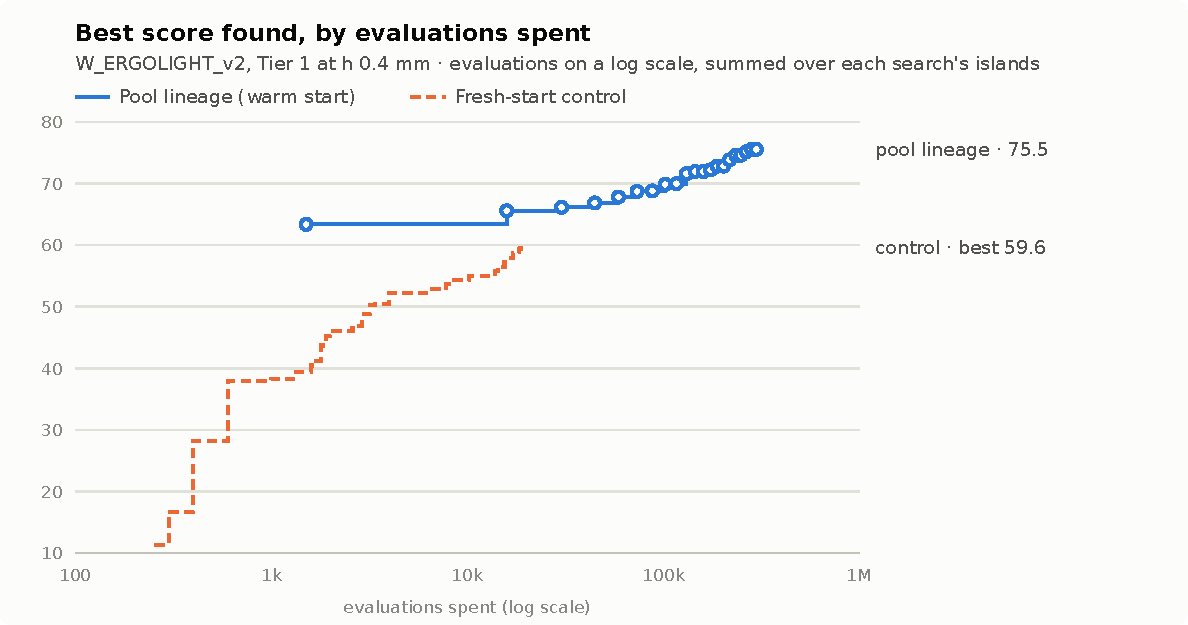
\includegraphics[width=\linewidth]{evolution.pdf}
\caption{Best \code{W\_ERGOLIGHT\_v2} score found against evaluations across all \gIslands{} evolving islands (winning island
\gWinIsland{} highlighted) against the scrambled-Sobol random-search control (\gBaselineBest{} max).}\label{fig:evo}
\end{figure}

\begin{figure*}[t]
\centering
% generated by g5-release-tex: best design of the winning island (v6: of the pool lineage) at each checkpoint
\begin{minipage}[t]{0.196\textwidth}\centering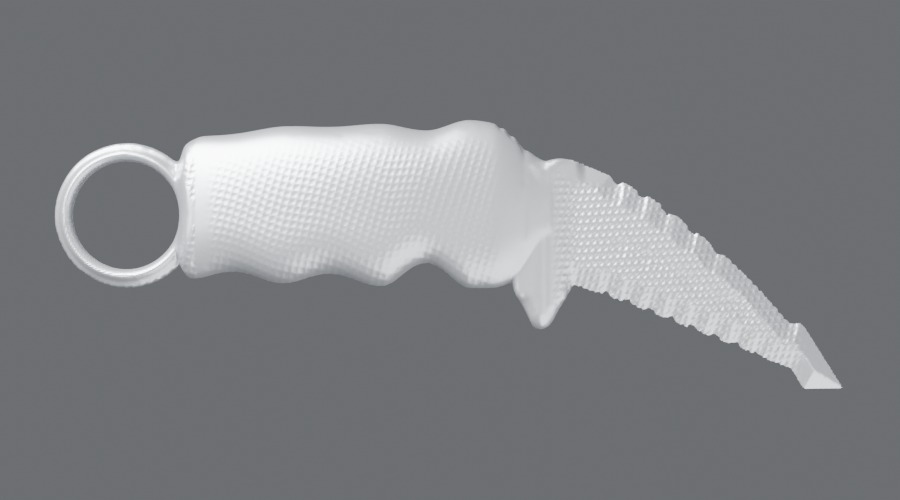
\includegraphics[width=\linewidth]{../../../docs/g5/v6.0.0/img/lineage_epoch00_pool.jpg}\\[-1pt]{\EItablefont pool epoch00/pool\\ 63.36, 103.6 g\\ \textbf{warm start}}\end{minipage}\hfill
\begin{minipage}[t]{0.196\textwidth}\centering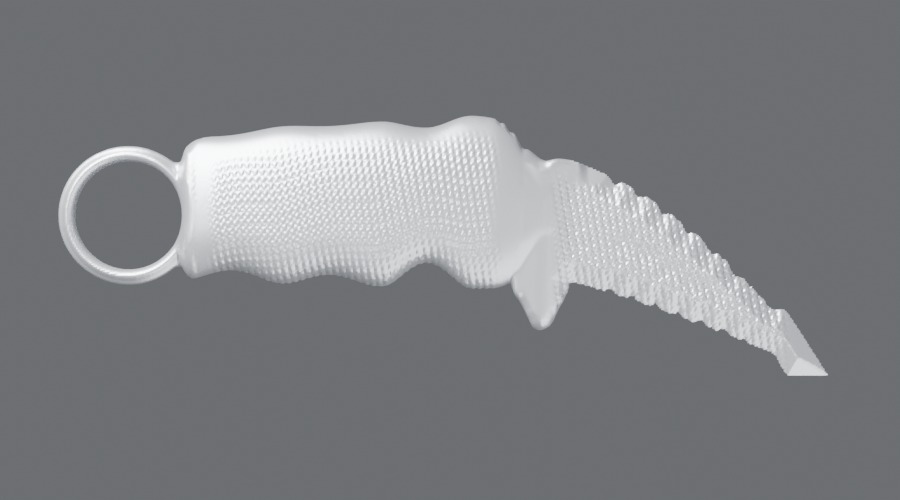
\includegraphics[width=\linewidth]{../../../docs/g5/v6.0.0/img/lineage_p04.jpg}\\[-1pt]{\EItablefont pool pools/p04\\ 67.81, 95.9 g}\end{minipage}\hfill
\begin{minipage}[t]{0.196\textwidth}\centering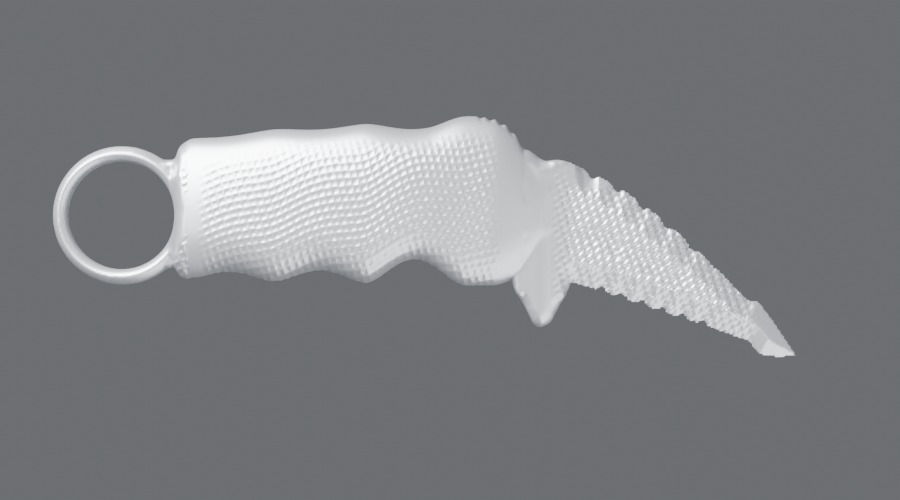
\includegraphics[width=\linewidth]{../../../docs/g5/v6.0.0/img/lineage_p10.jpg}\\[-1pt]{\EItablefont pool pools/p10\\ 71.94, 96.2 g}\end{minipage}\hfill
\begin{minipage}[t]{0.196\textwidth}\centering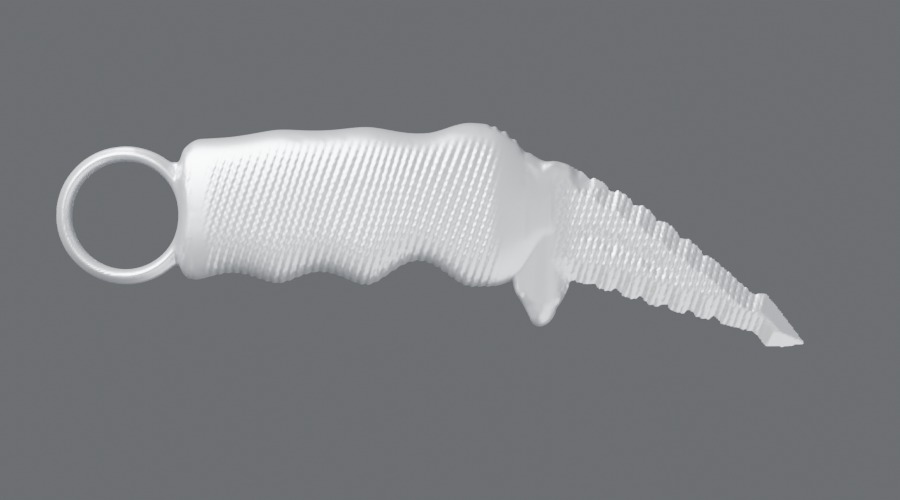
\includegraphics[width=\linewidth]{../../../docs/g5/v6.0.0/img/lineage_p14.jpg}\\[-1pt]{\EItablefont pool pools/p14\\ 72.81, 90.7 g}\end{minipage}\hfill
\begin{minipage}[t]{0.196\textwidth}\centering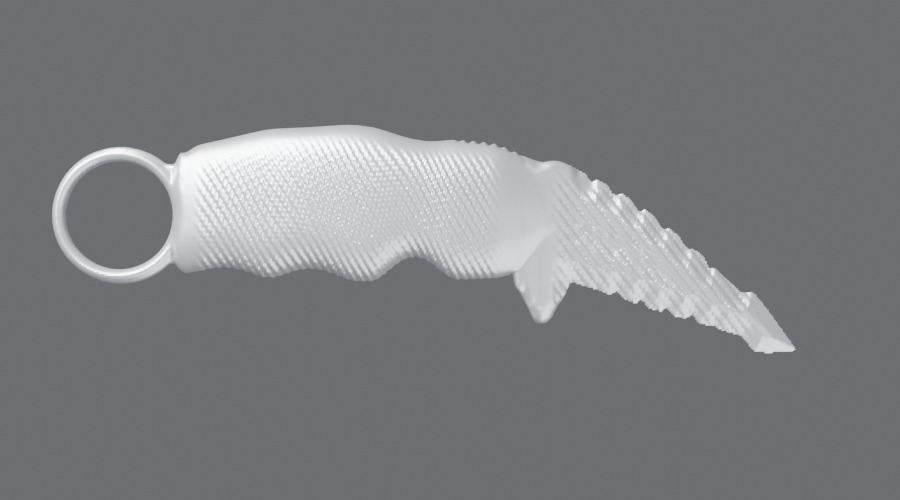
\includegraphics[width=\linewidth]{../../../docs/g5/v6.0.0/img/lineage_p20.jpg}\\[-1pt]{\EItablefont pool pools/p20\\ 75.54, 88.6 g\\ \textbf{final pool}}\end{minipage}\hfill

\caption{Best design of \gWinIsland{} at each logged checkpoint: evaluation count, \code{W\_ERGOLIGHT\_v2} score, and mass on
the search grid. Fixed camera, lighting and material across all frames.}\label{fig:lineage}
\end{figure*}

\subsection{Grid check and final Tier-2 ranking}
To verify grid independence, the top designs were evaluated across five voxel pitches $h \in \{0.4, 0.3, 0.25, 0.2, 0.15\}$~mm
(Table~\ref{tab:grid}). With smoothed-Heaviside partial-volume integration and width-aware drainage, the $0.20$~mm and
$0.15$~mm grids agree within \gGridAgree\,\%, and the search's $0.40$~mm mass matches the $0.20$~mm mass of record within
\gGridSpanPct\,\%. Table~\ref{tab:top} lists the top designs from the final Tier-2 ranking (shortlist \gShortlist) at
$h = \gHRank$~mm and $0.08~\mathrm{mm^2}$ solid-tip mesh resolution; the top eight rows span \gScore--\gTopLast. Re-ranking
the shortlist at Tier~2 is essential: the search-grid leader \gSearchLeaderId{} (\gSearchLeaderTierOne{} at Tier~1, where the 1D
section model estimated tip axial SF~\gSearchLeaderTipSecAx) drops to rank~\gSearchLeaderRank{} at Tier~2 (\gSearchLeaderTierTwo)
because its 3D \code{TET10} solid-tip submodel carries the $\gReqTipAxN$~N axial case at SF~\gSearchLeaderTipSolAx{} (margin
$v = \gSearchLeaderMargin$ against the $\gReqSfYield$ requirement).

\begin{table}[t]
\caption{Grid check: partial-volume mass (g) of the top designs across five voxel pitches $h$ (mm)}\label{tab:grid}
\centering
\begin{tabular}{@{}lrrrrr@{}}
\toprule
Design & 0.4 & 0.3 & 0.25 & 0.2 & 0.15 \\
\midrule
\gGridRows
\bottomrule
\end{tabular}
\end{table}

\begin{table}[t]
\caption{Final ranking: Tier 2 at $h = \gHRank$ mm and $0.08~\mathrm{mm^2}$ solid-tip mesh}\label{tab:top}
\centering
\begin{tabular}{@{}rlrrr@{}}
\toprule
Rank & Design & Score & $W$ & Mass (g) \\
\midrule
\gTopEightRows
\bottomrule
\end{tabular}
\end{table}

\begin{figure*}[t]
\centering
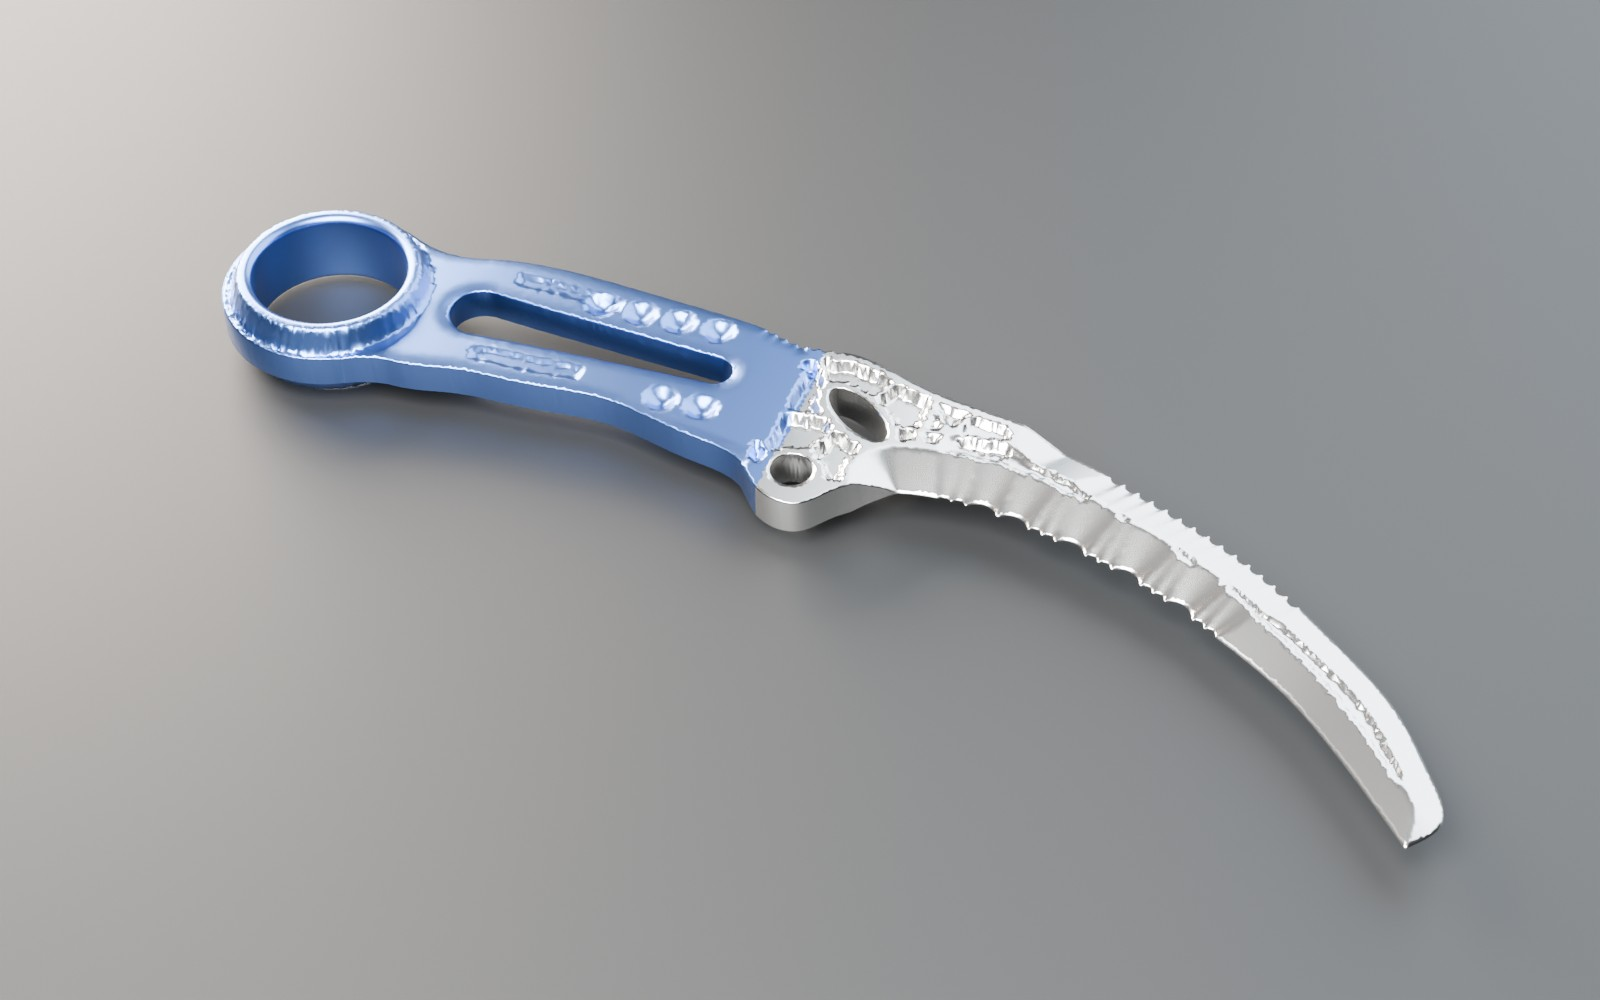
\includegraphics[width=0.49\textwidth]{hero.jpg}\hfill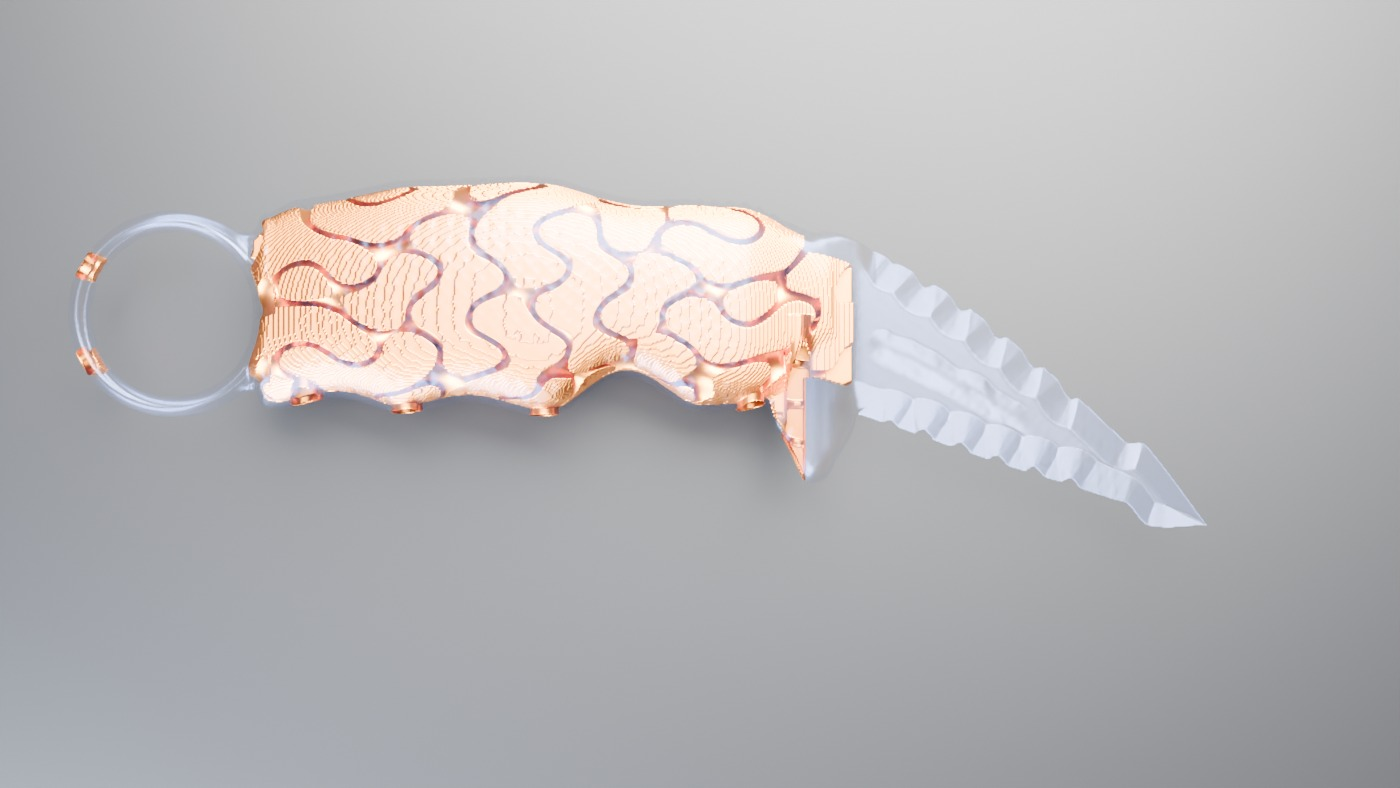
\includegraphics[width=0.49\textwidth]{xray.jpg}\\[3pt]
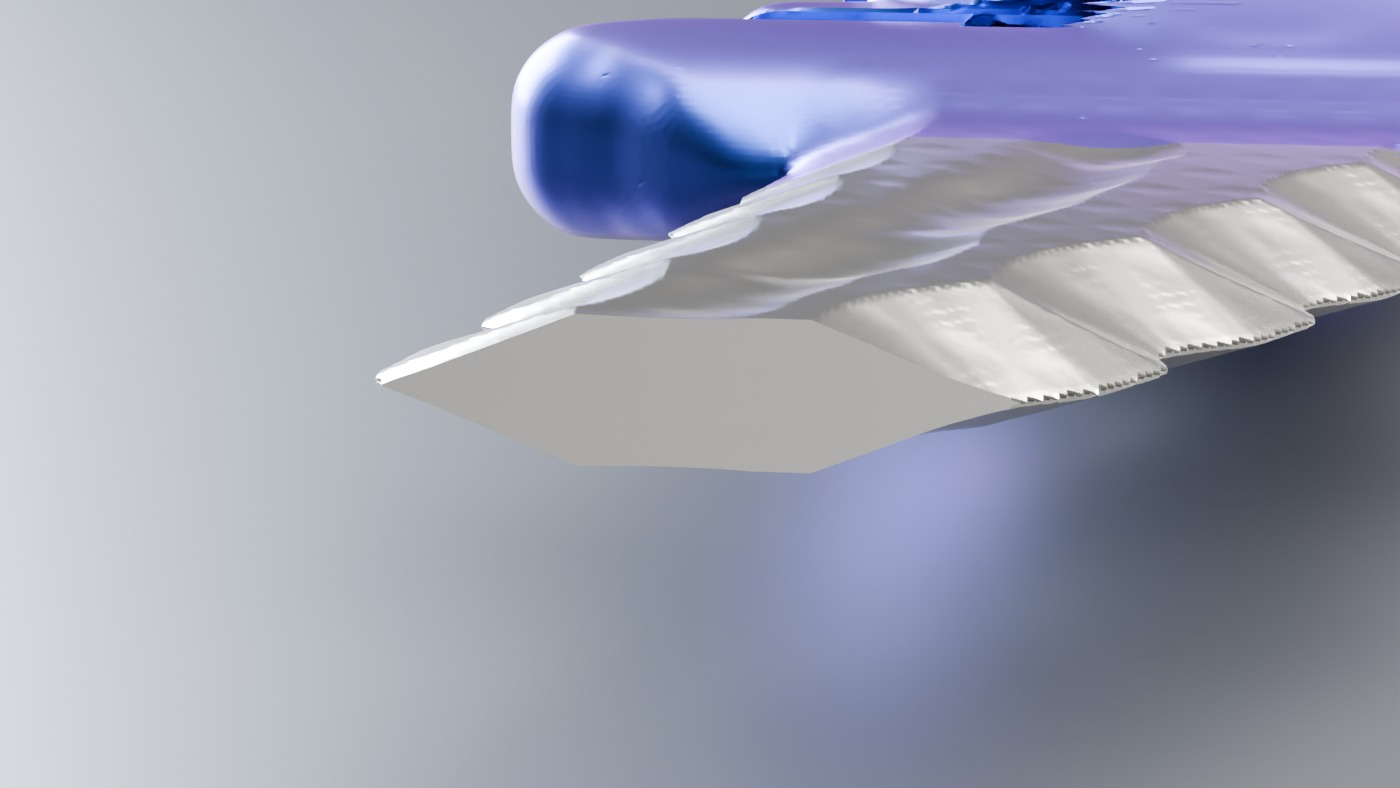
\includegraphics[width=0.32\textwidth]{cut_b.jpg}\hfill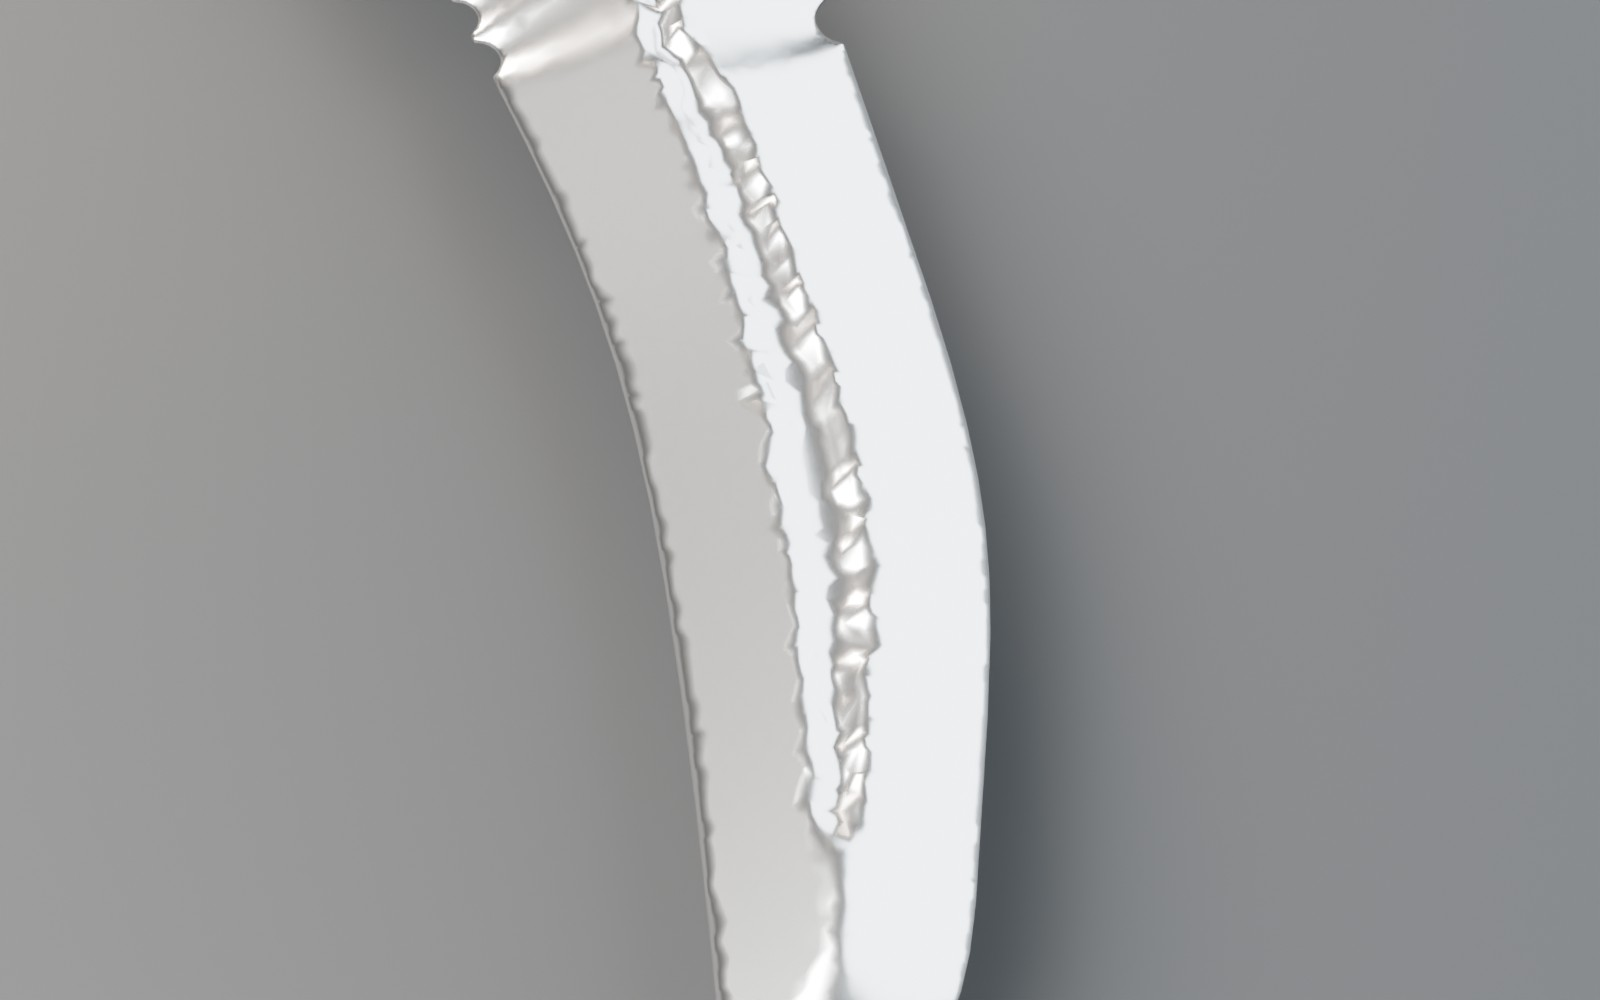
\includegraphics[width=0.32\textwidth]{tip.jpg}\hfill
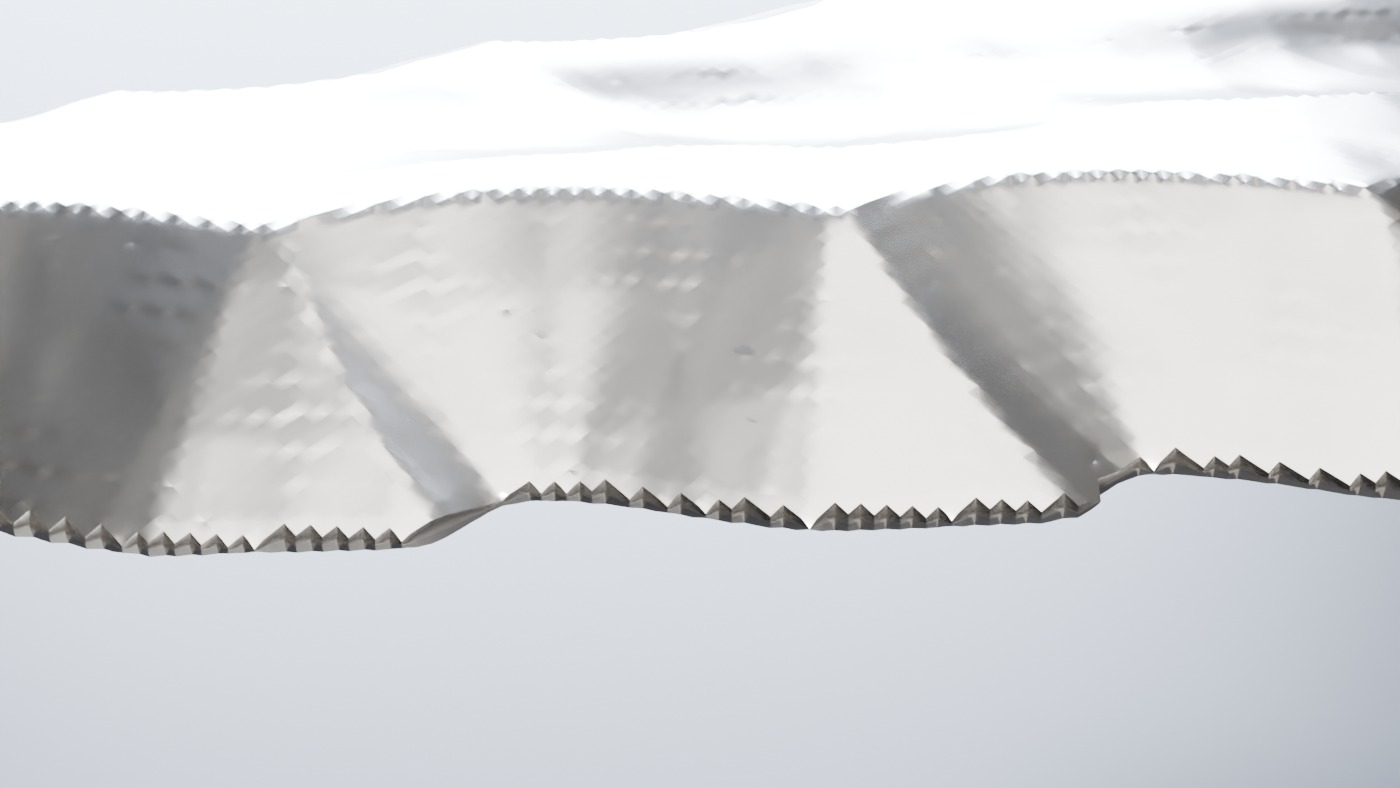
\includegraphics[width=0.32\textwidth]{edge_b.jpg}
\caption{\gDesign. Top: three-quarter view as decoded (before grinding), and an x-ray cutaway showing the internal sheet-TPMS
cavities and rib-clear drainage ports in amber. Bottom: cross-section across the blade 30~mm from the point, the sharp point
wedge, and the spine edge with its rounded-gullet serrations, as decoded (before grinding).}\label{fig:hero}
\end{figure*}

\subsection{The best individual (\gDesign)}
The winning individual, \gDesign{} (genome hash \gGenomeSha), scores \gScore{} under \code{W\_ERGOLIGHT\_v2} with weighted base
\gBase, ergonomic multiplier $E = \gE$ ($E^5 = \gEFive$), and worst-margin multiplier $W = \gW$ (worst safety-factor ratio
$\mu = \gWorstMarginRatio$ on \gWorstMarginCase). Its finished partial-volume mass of record at $h = \gHRank$~mm is
\gMassFinishedG{}~g (\gMassG{}~g on the watertight print mesh; solid outer envelope \gVolEnv{}~$\mathrm{mm^3}$, \gMassEnvG{}~g).
Its grip is \gLg{}~mm long with a swell perimeter of \gSwellPerim{}~mm ($84$--$100$~mm target band) and height-to-thickness ratio
\gHoT{} ($1.5$--$1.8$ target band); the guard is \gGuardH{}~mm high and the straight-line blade reach is \gReach{}~mm. Internal
sealed void volume is \gSealedVoid{}~$\mathrm{mm^3}$ (open surface crevices \gCreviceVoid{}~$\mathrm{mm^3}$), drained through
\gPortCount{} ports of diameter \gPortD{}~mm. Because the genome scopes the evolved surface texture onto the blade
(\code{scope\_blade} $= \gScopeBlade$, depth $\gTexAmp$~mm, pitch $\gTexPitch$~mm), the as-decoded renders and print meshes show
knurling across the blade flats and bevels; the analytical edge cross-sections (Fig.~\ref{fig:edges}) and edge metrics evaluate
the bevel law restored after post-build grinding ($\gReqEdgeFinishMm$~mm finishing allowance per ground face). Fig.~\ref{fig:hero}
and Fig.~\ref{fig:edges} show its geometry;
Table~\ref{tab:best} reports all 16 structural load cases and key geometric measurements against \code{RS-karambit-v5}.

\begin{table}[t]
\caption{Measurements and safety factors of the best individual \gDesign{} against \code{RS-karambit-v5}}\label{tab:best}
\centering
\EItablefont
\setlength{\tabcolsep}{2.2pt}
\begin{tabular}{@{}lrrr@{}}
\toprule
Quantity / Load case & Value & Req. & $v$ \\
\midrule
Score (\code{W\_ERGOLIGHT\_v2}) & \gScore & --- & $E=\gE$ \\
Mass, partial vol.\ / mesh (g) & \gMassFinishedG{} / \gMassG & $\gReqMassGoal$ goal ($\le \gReqMassCeil$) & $W=\gW$ \\
Sealed void ($\mathrm{mm^3}$) / ports & \gSealedVoid{} / $\varnothing\gPortD$ & $0$ / $\ge \gReqPortD$ & $N=\gPortCount$ \\
Grip $L_g$ / perim.\ (mm) / $H/T$ & \gLg{} / \gSwellPerim{} / \gHoT & $\ge \gReqLg$ / $\gReqPerimMin$--$\gReqPerimMax$ & $\gReqHoTMin$--$\gReqHoTMax$ \\
Guard $h$ / CoM to choil (mm) & \gGuardH{} / \gComIdx & $\ge \gReqGuardH$ / $\le \gReqComIdx$ & --- \\
Point angle $1$ / $3$~mm (\textdegree) & \gPointAngleOne{} / \gPointAngleThree & $\le \gReqPtOne$ / $\le \gReqPtThree$ & $w_2=\gPointWidthTwo$ \\
Edge A / B grind (\textdegree, max \gEdgeMaxAngle) & \gEdgeAAngle{} / \gEdgeBAngle & $\gReqEdgeMin$--$\gReqEdgeMax^\circ$ & flat \gEdgeMaxApex \\
Serr.\ depth (mm), scallops A / B & \gEdgeADepth{} (\gEdgeATeeth) / \gEdgeBDepth{} (\gEdgeBTeeth) & $\gReqSerrMin$--$\gReqSerrMax$, $\ge \gReqScallopsMin$ & $r_g \ge \gReqGulletR$ \\
\midrule
Lateral limit ($\gReqLatLimNm$~N$\cdot$m, plate) & SF \gLoadLatLim & $\ge \gReqSfYield$ & \gMarginLatLim \\
Lateral ult.\ ($\gReqLatUltNm$~N$\cdot$m, plate) & SF \gLoadLatUlt & $\ge \gReqSfUlt$ & \gMarginLatUlt \\
Body twist ($\gReqTwistLimNm$~N$\cdot$m, plate) & SF \gLoadTwistLim & $\ge \gReqSfYield$ & \gMarginTwistLim \\
Tip axial ($\gReqTipAxN$~N, \code{TET10}) & SF \gLoadTipAxial & $\ge \gReqSfYield$ & \gMarginTipAxial \\
Tip lateral ($\gReqTipLatN$~N, \code{TET10}) & SF \gLoadTipLat & $\ge \gReqSfYield$ & \gMarginTipLat \\
Tip twist ($\gReqTipTwNm$~N$\cdot$m, \code{TET10}) & SF \gLoadTipTwist & $\ge \gReqSfYield$ & \gMarginTipTwist \\
Grip squeeze ($\gReqGripSqN$~N) & SF \gLoadGripSqueeze & $\ge \gReqSfYield$ & \gMarginGripSqueeze \\
Guard slip push ($\gReqGuardPushN$~N) & SF \gLoadGuardPush & $\ge \gReqSfYield$ & \gMarginGuardPush \\
Ring bearing ($\gReqRingBearN$~N, $\pm \gReqRingArcDeg^\circ$) & SF \gLoadRingBear & $\ge \gReqSfRing$ & \gMarginRingBear \\
Ring back ($\gReqRingBackN$~N) & SF \gLoadRingBack & $\ge \gReqSfRing$ & \gMarginRingBack \\
Ring in-plane sweep ($\gReqRingAnyN$~N) & SF \gLoadRingAny & $\ge \gReqSfYield$ & \gMarginRingAny \\
Axial pull ($\gReqPullN$~N, plate/grip) & SF \gLoadPull & $\ge \gReqSfYield$ & \gMarginPull \\
Serration teeth ($\gReqSnagN/\gReqPryN$~N, all) & SF \gLoadTeeth & $\ge \gReqSfYield$ & \gMarginTeeth \\
Fatigue ($10^6$ cyc, FKM class) & SF \gLoadFatigue & $\ge \gReqSfFat$ & \gMarginFatigue \\
Yield sequence ($\min$ per case) & \gLoadSeqMin & $\ge \gReqSeqRatio$ & \gMarginSeq \\
Tip buckling $\lambda$ ($\gReqTipAxN$~N, Ritz) & \gLoadBuckling & $\ge \gReqBuckling$ & \gMarginBuckling \\
\bottomrule
\end{tabular}
\end{table}

\begin{table}[t]
\caption{Verification studies (\code{evidence/g5/v\gRecord/vv/} and \code{release.json}): plate refinement, solid-tip
refinement and solver checks}\label{tab:vv}
\centering
\EItablefont
\setlength{\tabcolsep}{2.4pt}
\begin{tabular}{@{}llrrr@{}}
\toprule
Study & Quantity & Coarse & Med. & Fine \\
\midrule
Plate ($1.2/0.3/0.15~\mathrm{mm^2}$) & Lat.\ limit SF & \gVvPlateLatA & \gVvPlateLatB & \gVvPlateLatC \\
Plate ($1.2/0.3/0.15~\mathrm{mm^2}$) & Twist limit SF & \gVvPlateTwistA & \gVvPlateTwistB & \gVvPlateTwistC \\
Tip \code{TET10} (sec/$0.15/0.08$) & Axial SF & \gVvTipAxA & \gVvTipAxB & \gVvTipAxC \\
Tip \code{TET10} (sec/$0.15/0.08$) & Lateral SF & \gVvTipLatA & \gVvTipLatB & \gVvTipLatC \\
Tip \code{TET10} (sec/$0.15/0.08$) & Twist SF & \gVvTipTwA & \gVvTipTwB & \gVvTipTwC \\
Tier-1 determinism & Archive rows & \gCohortElites & --- & \gTierOneReproduced{} exact \\
Linux \code{x86\_64} Tier 2 & Max rel.\ diff & \gLinuxDesigns{} top & --- & \gLinuxMaxRelDiff \\
Ritz vs.\ Euler column & $|\Delta P_\mathrm{cr}|/P_\mathrm{cr}$ & --- & --- & \gVvRitzErr \\
\bottomrule
\end{tabular}
\end{table}

\begin{figure}[!t]
\centering
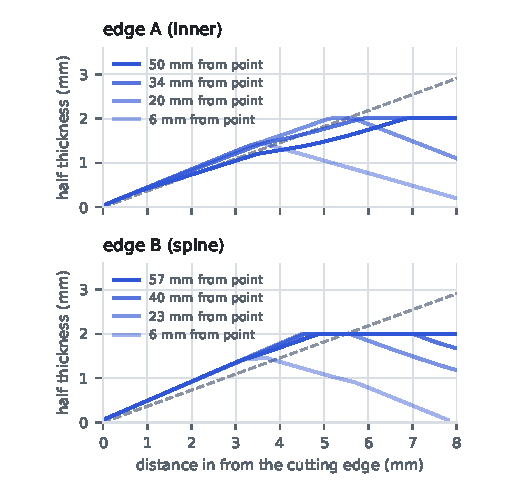
\includegraphics[width=\linewidth]{edge_sections.pdf}
\caption{Upper half of the blade cross-section at four stations along each edge of \gDesign, true scale, measured normal to
the serrated edge from the exact decoder law (dashed: $\gReqEdgeMin^\circ$ per side, the requirement's minimum).}\label{fig:edges}
\end{figure}

\section{FEM renderings of every load case}\label{sec:fem}
The scored solvers return safety factors and discard their fields. \src{crates/g5/src/bin/g5_fem_fields/main.rs}{\code{g5-fem-fields}}
re-solves each of the \gFemCases{} load cases of \gDesign{} on the ranking grid ($h = \gFemH$~mm) with copies of the scored models
(the whole-blade CST+DKT sandwich plate, the \code{TET10} solid tip, the \code{T6} ring with its twelve-direction sweep and the
Rayleigh--Ritz column, now with its mode) and keeps the fields: von Mises stress on a five-band sequential scale, the governing
point and the deformed shape (Figs.~\ref{fig:fem1} and~\ref{fig:fem2}). The \gFemReproduced{} scored values these solves produce
(the safety factors, the Ritz eigenvalue, the sequence ratios and the governing points) match the receipt bit for bit on the
platform of record; the tool fails if any does not.

The score models grip squeeze, guard push and teeth analytically. For those three, the figures show an independent hex8 voxel
finite-element solve on the design's own additive-manufacturing voxel field instead, reported beside the score model and not used by
it (Table~\ref{tab:hex8}).

\begin{table}[t]
\caption{Independent hex8 voxel FE against the score's analytic models (\gDesign; safety factor, required $\gReqSfYield$)}\label{tab:hex8}
\centering
\begin{tabular}{@{}lrr@{}}
\toprule
Case & Score model & Hex8 FE \\
\midrule
Grip squeeze ($\gReqGripSqN$~N) & \gFemModelGrip & \gFemHexGrip \\
Guard push ($\gReqGuardPushN$~N) & \gFemModelGuard & \gFemHexGuard \\
Serration teeth ($\gReqSnagN/\gReqPryN$~N) & \gFemModelTeeth & \gFemHexTeeth \\
\bottomrule
\end{tabular}
\end{table}

\begin{figure*}[p]
\centering
% generated by g5-release-tex from docs/g5/v<rv>/img/fem/figures.json
\begin{minipage}[t]{0.49\textwidth}\centering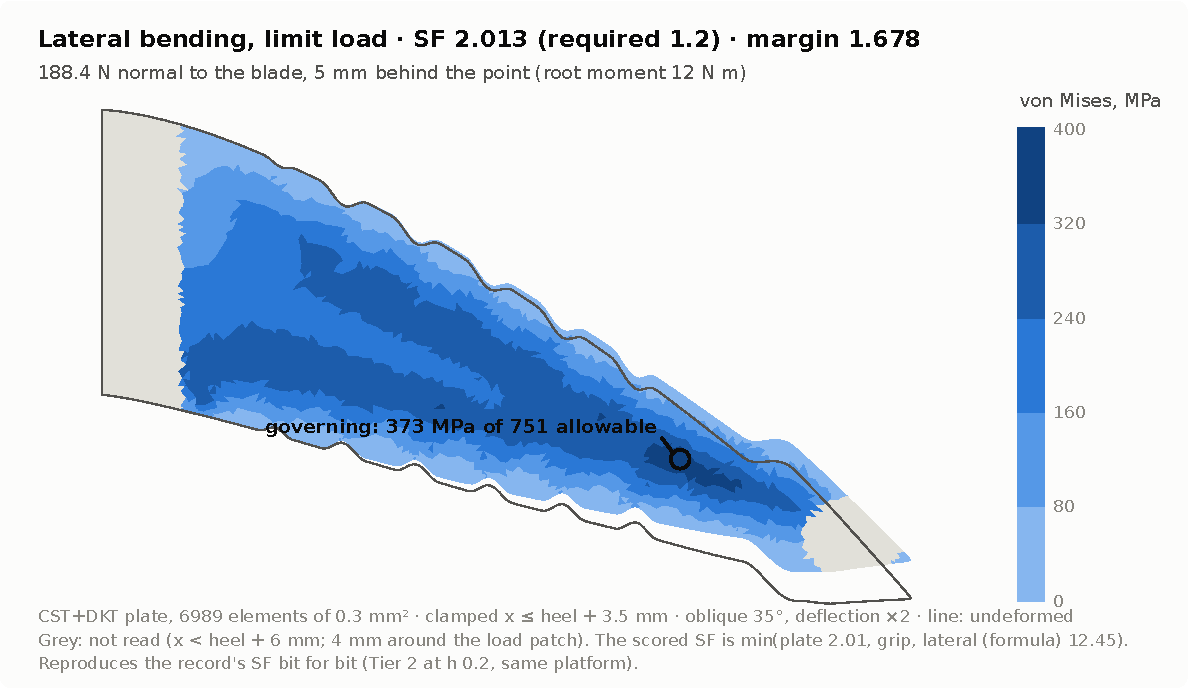
\includegraphics[width=\linewidth]{fem/lateral_limit.pdf}\\[-2pt]{\EItablefont Lateral bending, limit load: SF 2.01}\end{minipage}\hfill
\begin{minipage}[t]{0.49\textwidth}\centering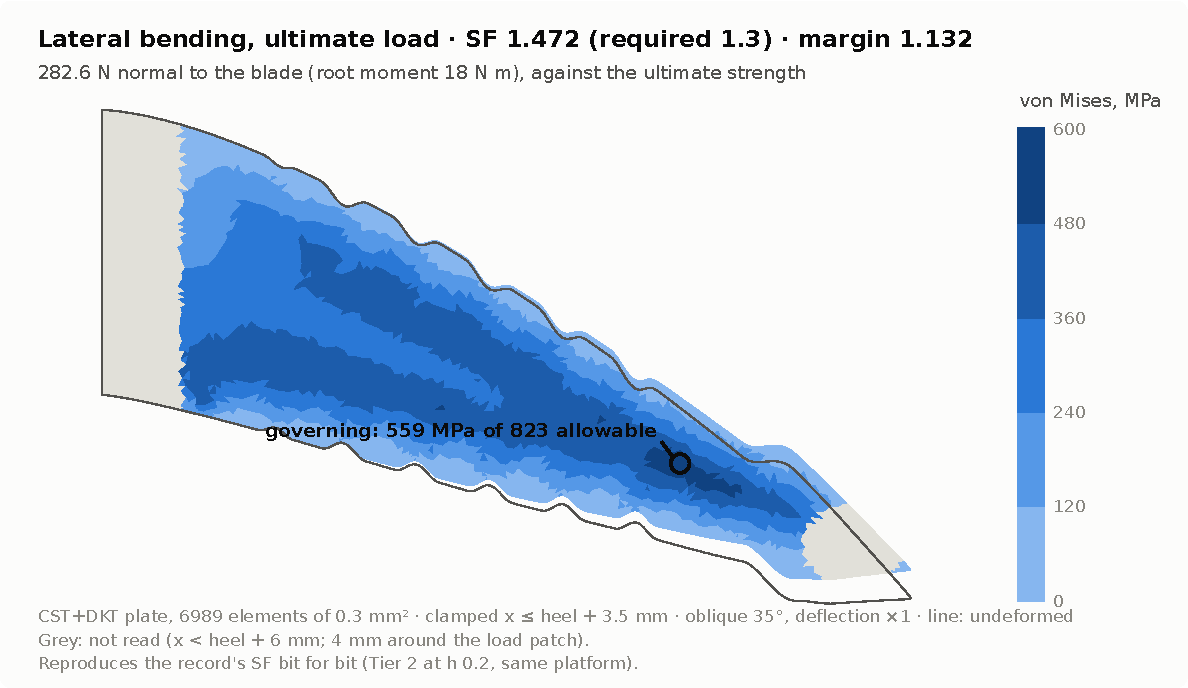
\includegraphics[width=\linewidth]{fem/lateral_ultimate.pdf}\\[-2pt]{\EItablefont Lateral bending, ultimate load: SF 1.47}\end{minipage}\\[4pt]
\begin{minipage}[t]{0.49\textwidth}\centering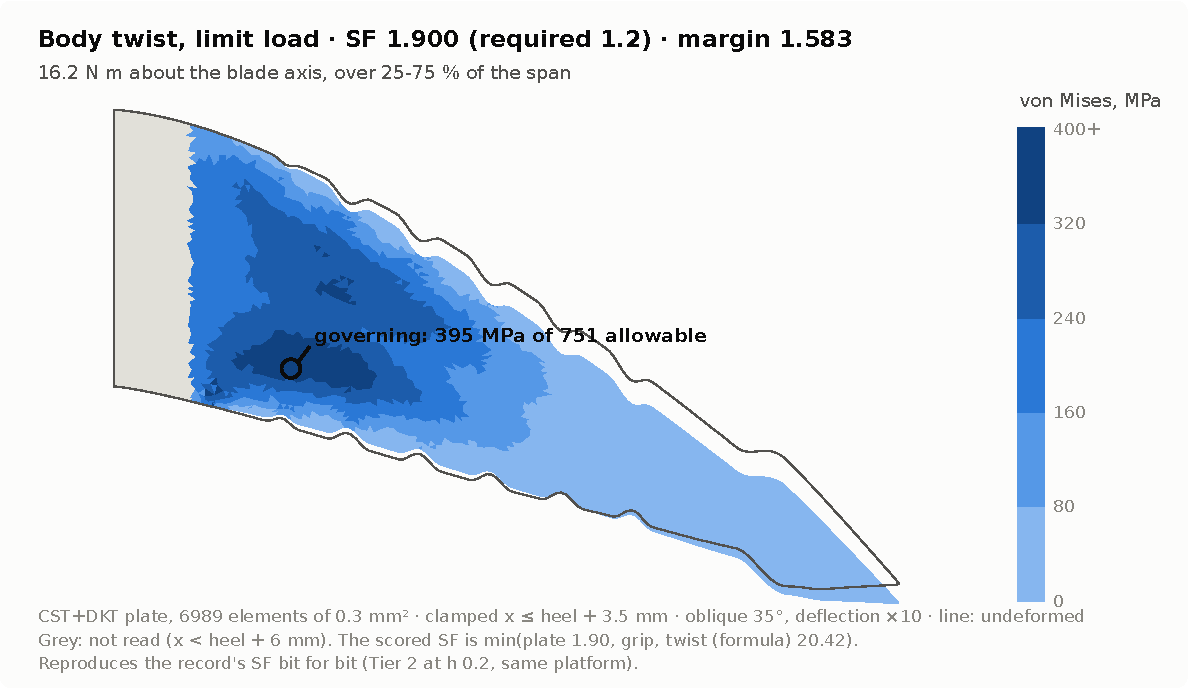
\includegraphics[width=\linewidth]{fem/twist_limit.pdf}\\[-2pt]{\EItablefont Body twist, limit load: SF 1.90}\end{minipage}\hfill
\begin{minipage}[t]{0.49\textwidth}\centering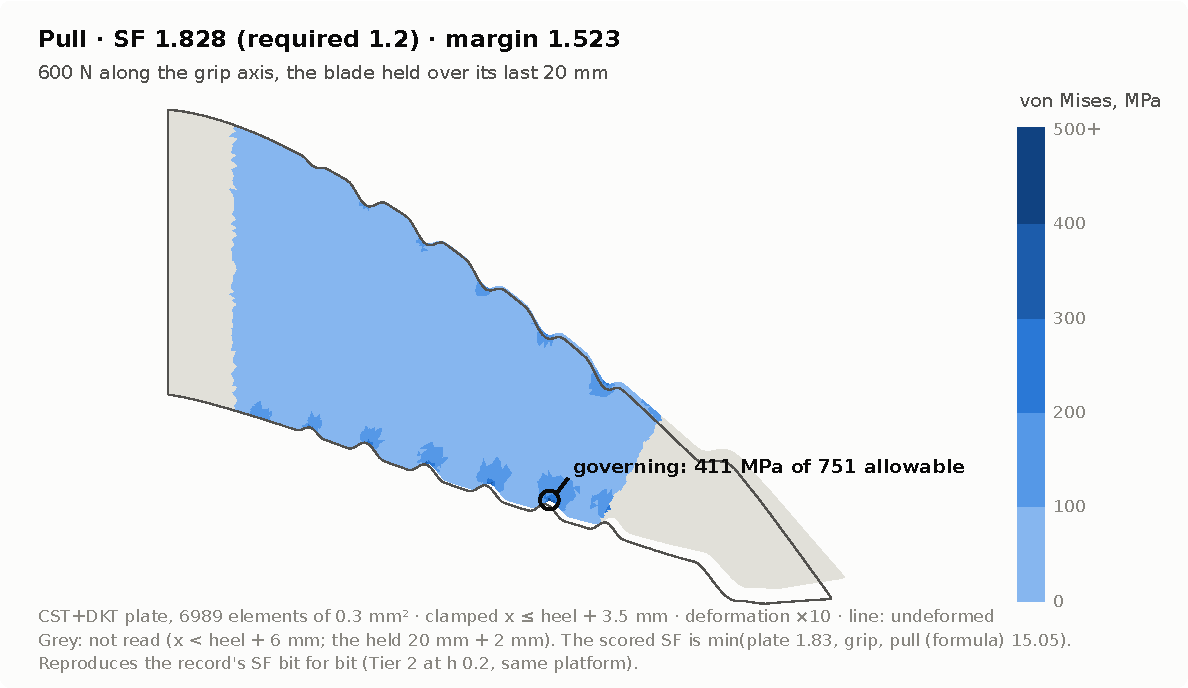
\includegraphics[width=\linewidth]{fem/pull.pdf}\\[-2pt]{\EItablefont Pull: SF 1.83}\end{minipage}\\[4pt]
\begin{minipage}[t]{0.49\textwidth}\centering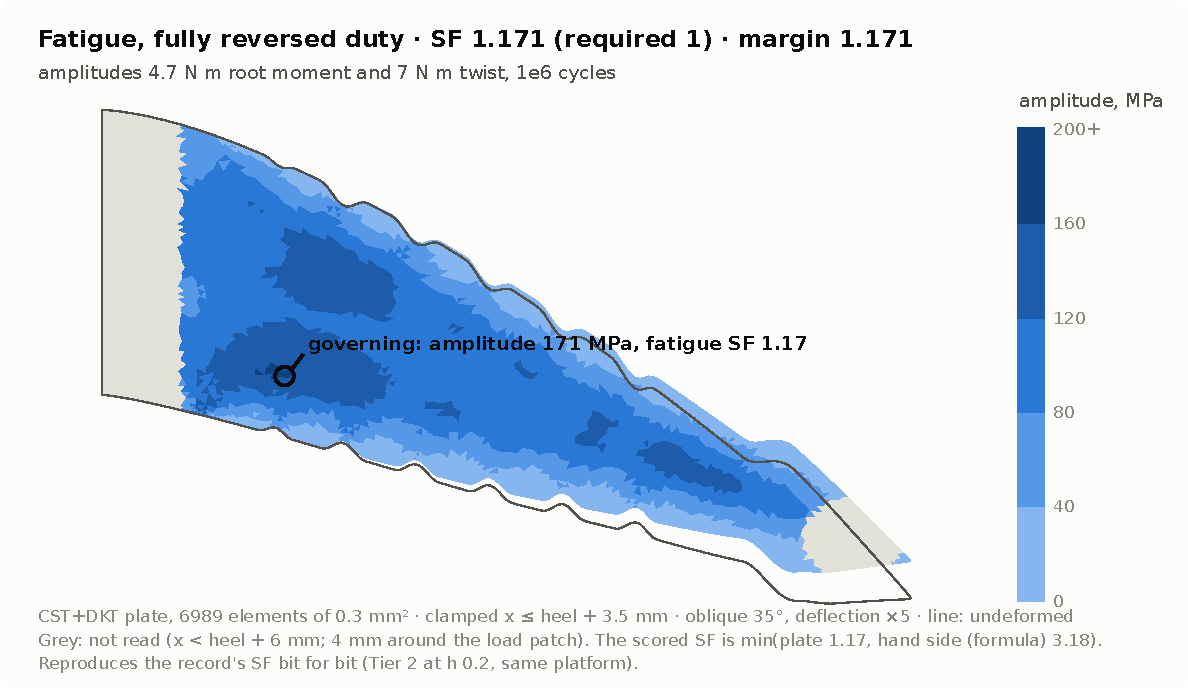
\includegraphics[width=\linewidth]{fem/fatigue.pdf}\\[-2pt]{\EItablefont Fatigue, fully reversed duty: SF 1.17}\end{minipage}\hfill
\begin{minipage}[t]{0.49\textwidth}\centering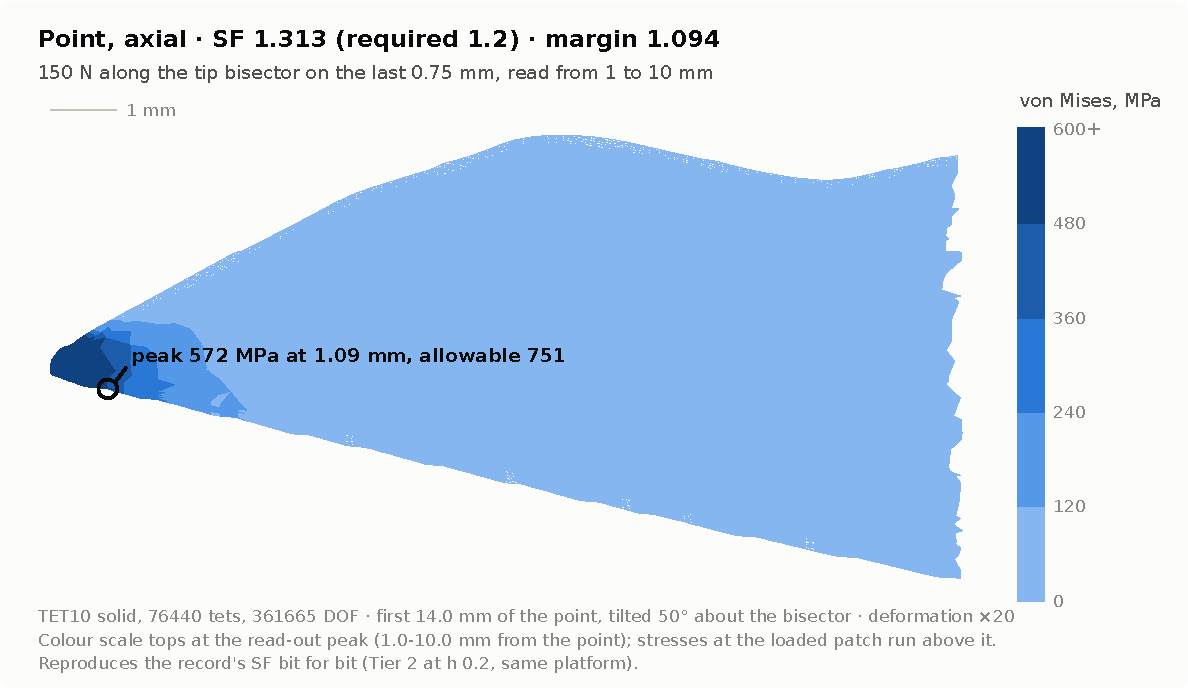
\includegraphics[width=\linewidth]{fem/tip_axial.pdf}\\[-2pt]{\EItablefont Point, axial: SF 1.31}\end{minipage}\\[4pt]
\begin{minipage}[t]{0.49\textwidth}\centering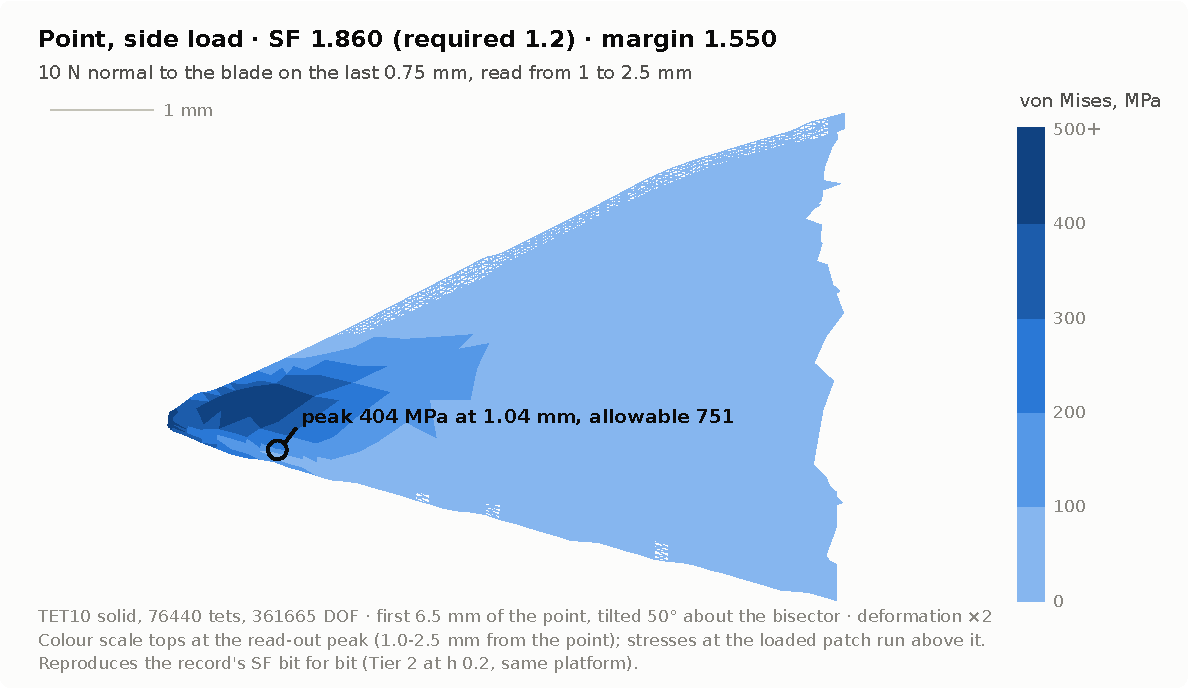
\includegraphics[width=\linewidth]{fem/tip_lateral.pdf}\\[-2pt]{\EItablefont Point, side load: SF 1.86}\end{minipage}\hfill
\begin{minipage}[t]{0.49\textwidth}\centering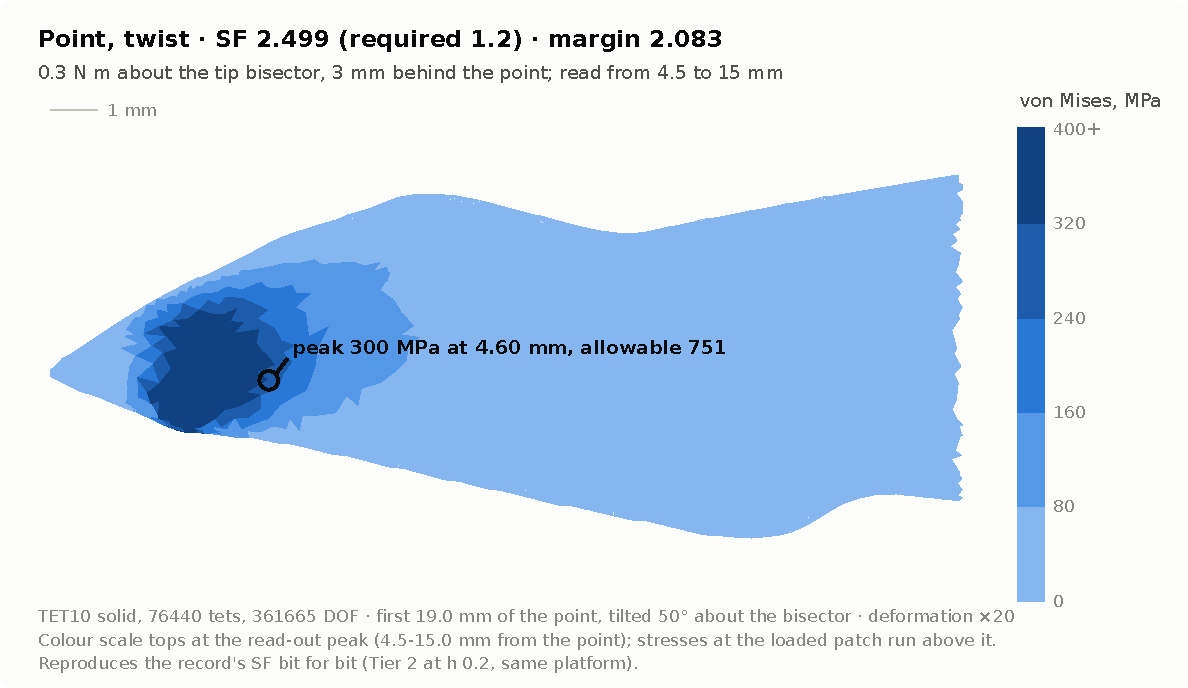
\includegraphics[width=\linewidth]{fem/tip_twist.pdf}\\[-2pt]{\EItablefont Point, twist: SF 2.50}\end{minipage}\\[4pt]

\caption{FEM renderings of the load cases of \gDesign{} (1 of 2): von Mises stress, governing point and deformed shape, as
re-solved by \code{g5-fem-fields}; each panel states its mesh, load and safety factor.}\label{fig:fem1}
\end{figure*}

\begin{figure*}[p]
\centering
% generated by g5-release-tex from docs/g5/v<rv>/img/fem/figures.json
\begin{minipage}[t]{0.49\textwidth}\centering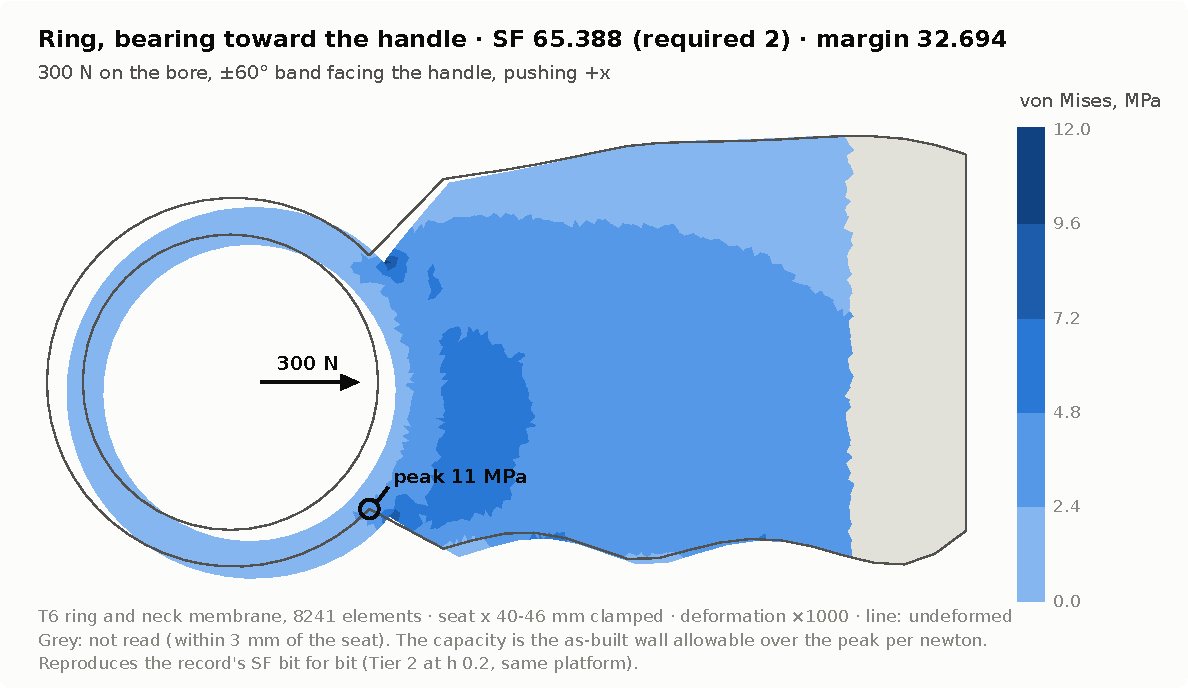
\includegraphics[width=\linewidth]{fem/ring_bearing.pdf}\\[-2pt]{\EItablefont Ring, bearing toward the handle: SF 65.39}\end{minipage}\hfill
\begin{minipage}[t]{0.49\textwidth}\centering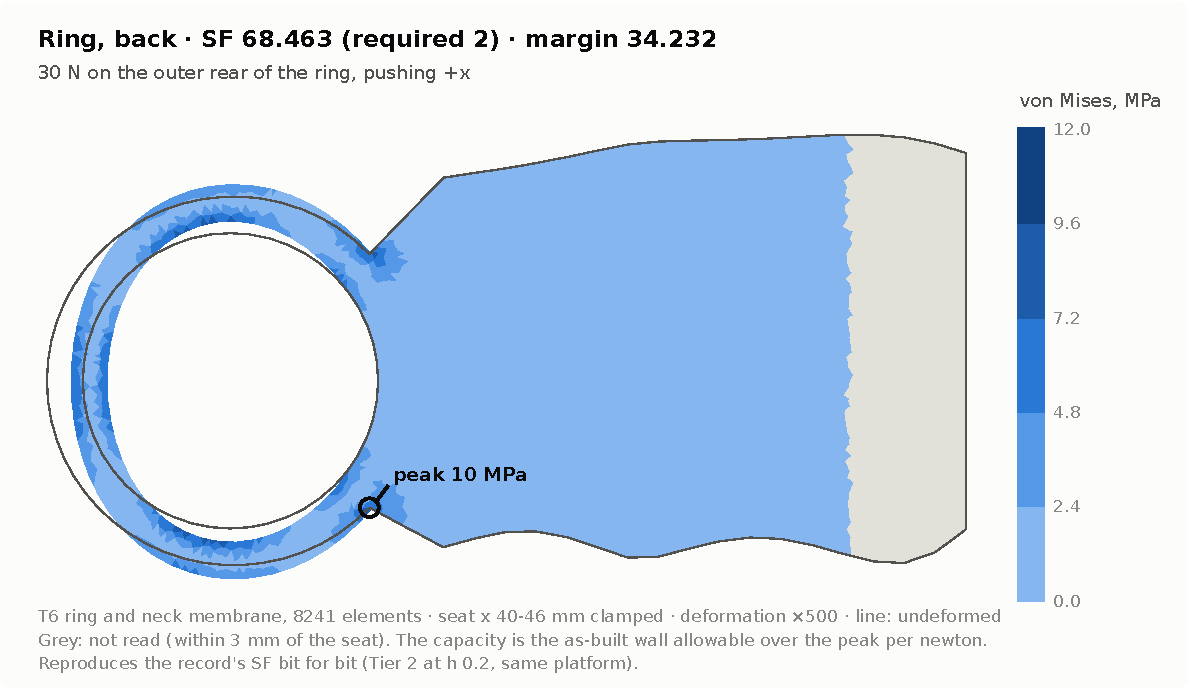
\includegraphics[width=\linewidth]{fem/ring_back.pdf}\\[-2pt]{\EItablefont Ring, back: SF 68.46}\end{minipage}\\[4pt]
\begin{minipage}[t]{0.49\textwidth}\centering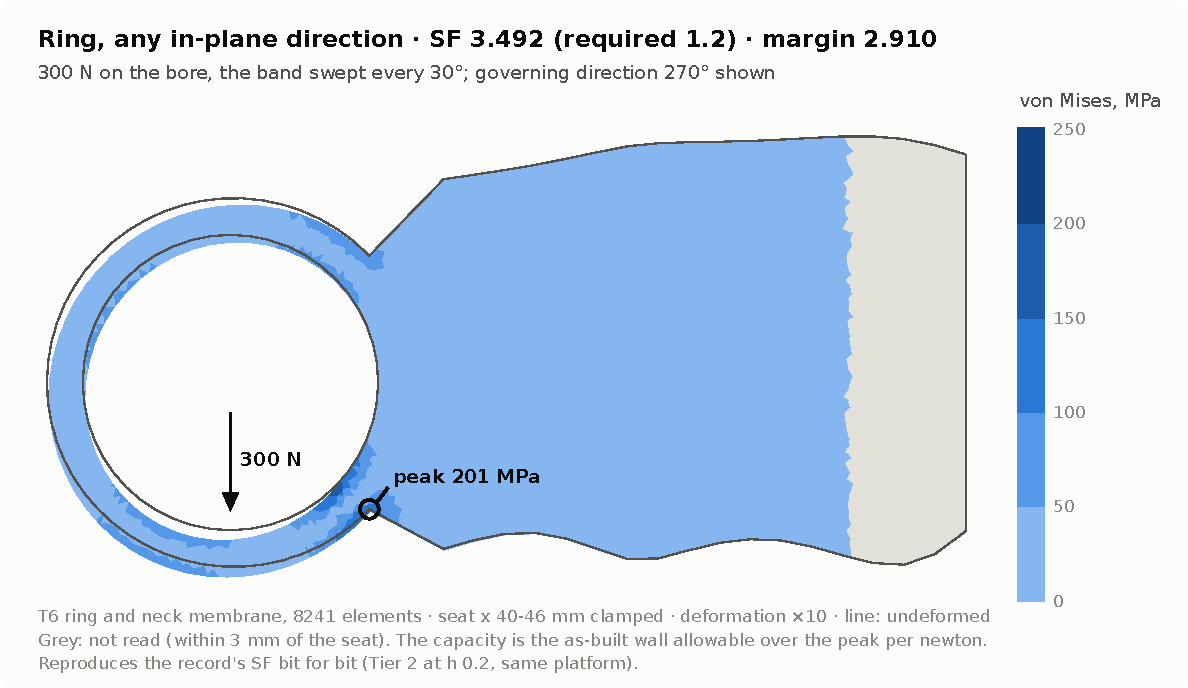
\includegraphics[width=\linewidth]{fem/ring_any_direction.pdf}\\[-2pt]{\EItablefont Ring, any in-plane direction: SF 3.49}\end{minipage}\hfill
\begin{minipage}[t]{0.49\textwidth}\centering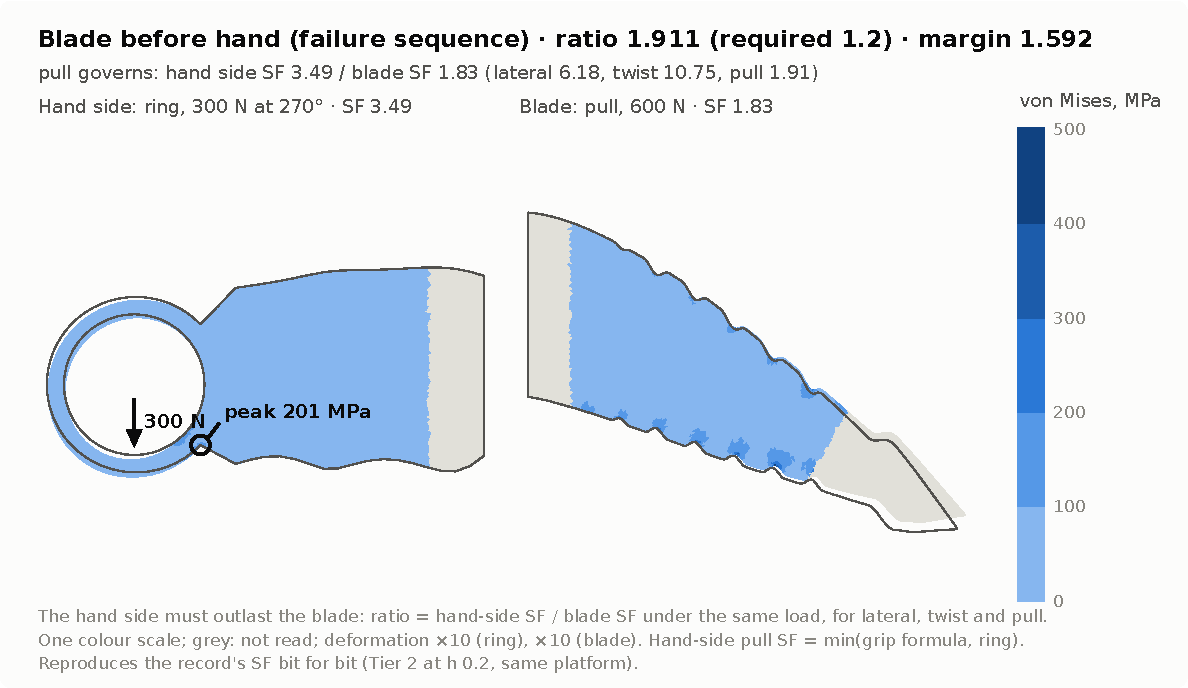
\includegraphics[width=\linewidth]{fem/sequence.pdf}\\[-2pt]{\EItablefont Blade before hand (failure sequence): SF 1.91}\end{minipage}\\[4pt]
\begin{minipage}[t]{0.49\textwidth}\centering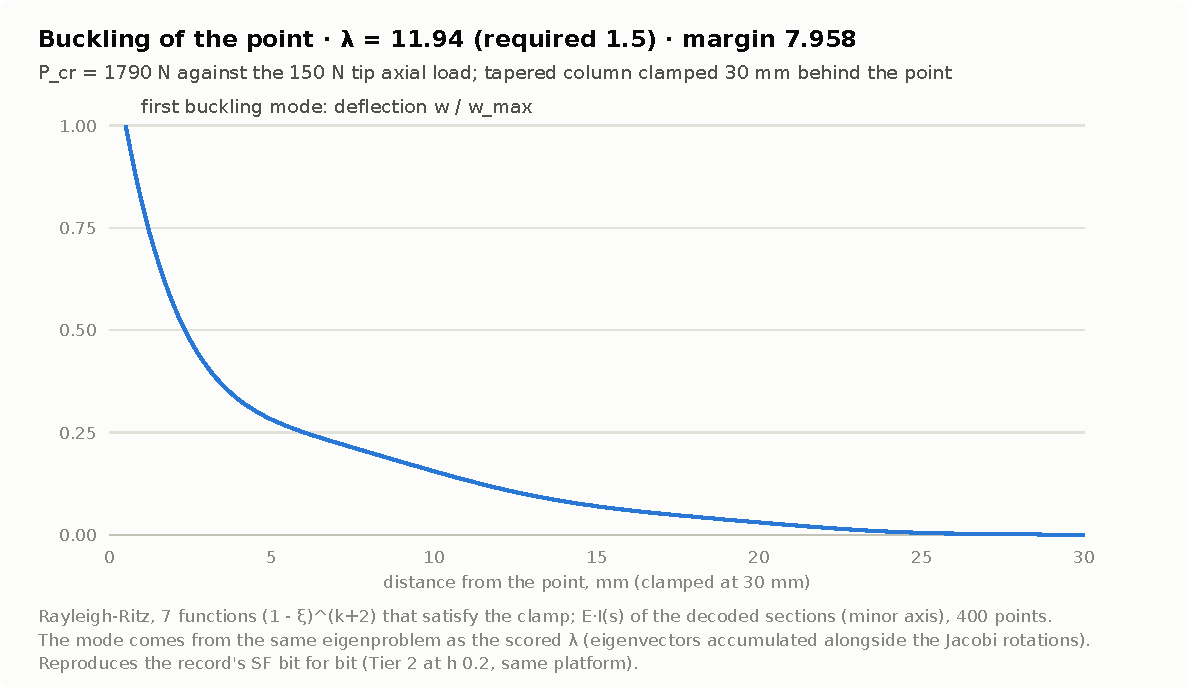
\includegraphics[width=\linewidth]{fem/buckling.pdf}\\[-2pt]{\EItablefont Buckling of the point: SF 11.94}\end{minipage}\hfill
\begin{minipage}[t]{0.49\textwidth}\centering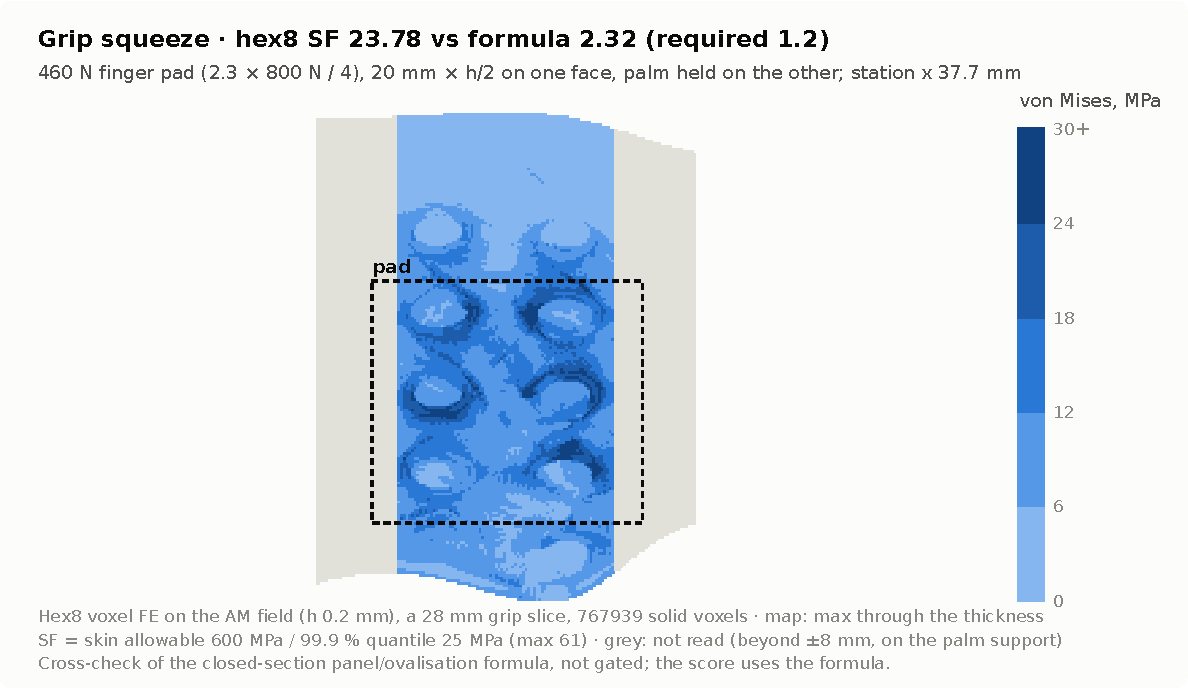
\includegraphics[width=\linewidth]{fem/grip_squeeze.pdf}\\[-2pt]{\EItablefont Grip squeeze: hex8 FE SF 23.78 (score model 2.32)}\end{minipage}\\[4pt]
\begin{minipage}[t]{0.49\textwidth}\centering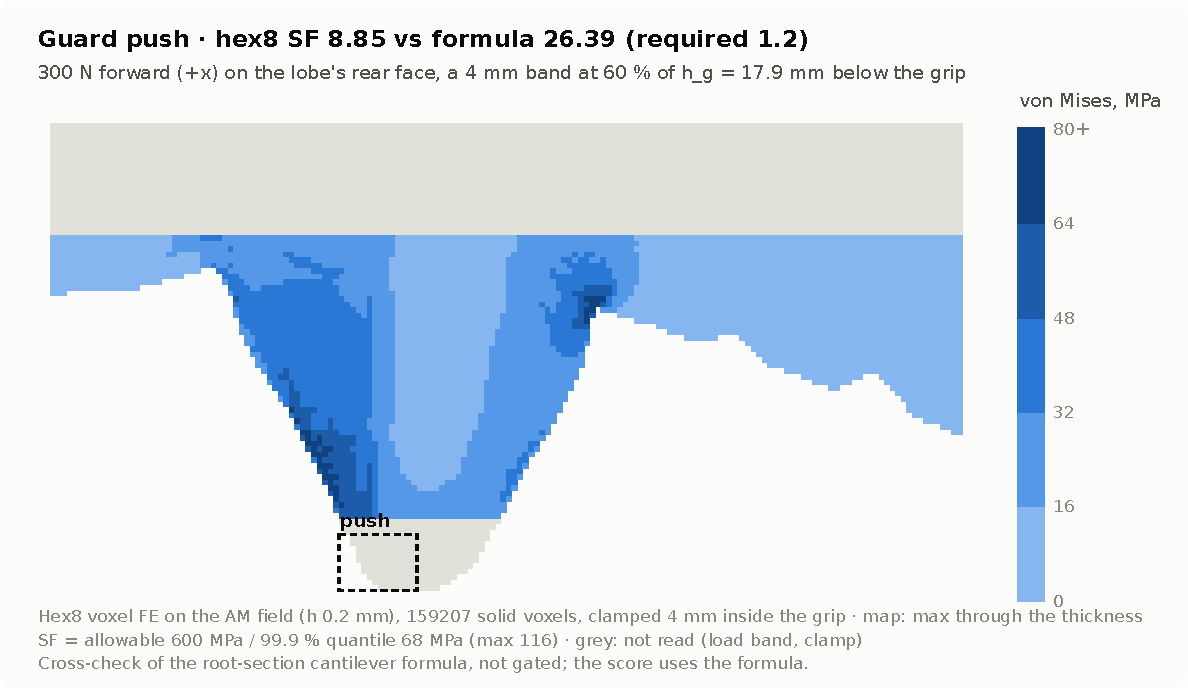
\includegraphics[width=\linewidth]{fem/guard_push.pdf}\\[-2pt]{\EItablefont Guard push: hex8 FE SF 8.85 (score model 26.39)}\end{minipage}\hfill
\begin{minipage}[t]{0.49\textwidth}\centering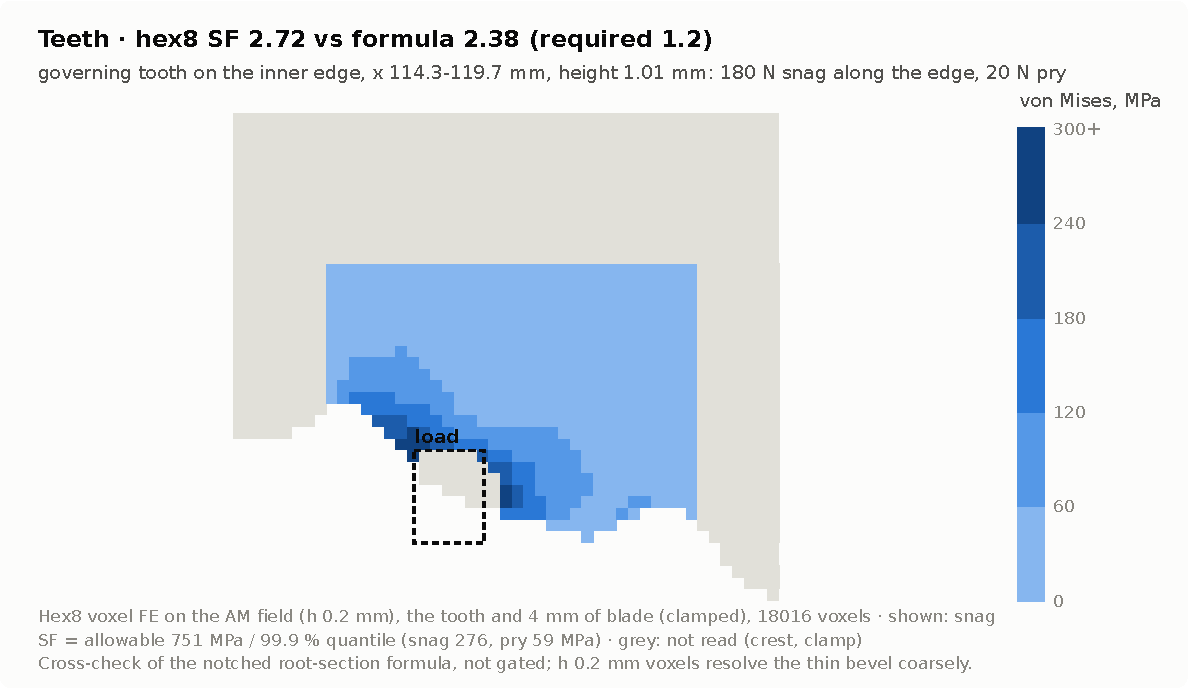
\includegraphics[width=\linewidth]{fem/teeth.pdf}\\[-2pt]{\EItablefont Teeth: hex8 FE SF 2.72 (score model 2.38)}\end{minipage}\\[4pt]

\caption{FEM renderings of the load cases of \gDesign{} (2 of 2), including the hex8 checks of the analytic cases.}\label{fig:fem2}
\end{figure*}

\section{Limits of the result and evidence gaps}\label{sec:limits}
\begin{eibox}{What this result is not}
It is a computational design (\gStatus). Nothing has been printed, stress-relieved, ground or physically tested, and no
safety factor reported here is a qualification for use.
\end{eibox}
\begin{itemize}
\item \textbf{Outcome against the targets.} The best individual \gDesign{} has worst safety-factor margin ratio
$\mu = \gWorstMarginRatio$ (on \gWorstMarginCase, multiplier $W = \gW$), finished partial-volume mass \gMassFinishedG{}~g
(\gMassG{}~g on the $0.20$~mm mesh, which \gMassReading), and sealed internal void volume \gSealedVoid{}~$\mathrm{mm^3}$
(printed solid in the build field, $d_\mathrm{am} = -h$, so the mass counts solid titanium rather than trapped powder).
\item \textbf{Blade surface texture (frozen \code{G5.0} decoder limit).} The frozen \code{G5.0} decoder allows the evolved
surface texture to reach the blade zone (for \gDesign, texture depth \code{tex\_amp} $= \gTexAmp$~mm, pitch $\gTexPitch$~mm, and
\code{scope\_blade} $= \gScopeBladeThree$), carving inward across both the blade flats and the bevels so the as-decoded edge is
notched. The edge cross-sections (Fig.~\ref{fig:edges}) and edge measurements evaluate the exact bevel law, which post-build
grinding restores because the \code{RS-karambit-v5} finishing allowance ($\gReqEdgeFinishMm$~mm per ground face) exceeds the
$\gTexAmp$~mm texture depth. Restricting surface texture outside the bevels is deferred to a later decoder generation.
\item \textbf{One platform of record.} v5.0.0's \code{arm64} records agreed closely with, but were not bit-identical to,
\code{x86\_64} re-evaluations, because the platforms' maths libraries differ in the last bits. v\gRecord{} runs the search, every
re-evaluation and the ranking on one platform (static \code{x86\_64} binaries, natively or in a \code{linux/amd64} container): every archive
row re-scores bit for bit, every pool is recomputed from its sources, \gReproIsland{} re-run on \gReproHost{} reproduced all
\gReproEntries{} logged history entries over \gReproEvals{} evaluations, and re-evaluating all \gCohortElites{} elites of the final
pool reproduced all \gTierOneReproduced{} Tier-1 rows. A different libm (another platform) would again agree closely rather than
exactly.
\item \textbf{The search grid can rank designs it cannot keep.} The search scores at $h = \gH$~mm with a section model of the tip;
the ranking re-scores the shortlist at $h = \gHRank$~mm with the solid tip and the winner must also pass the grid check and every
load case on every plate mesh. A design that leads the search grid can therefore rank lower, which is why the search-grid best of the
lineage (\gPoolFinalBest) is not the score of record (\gScore).
\item \textbf{Analytic hand-zone models, checked by FE.} The score models grip squeeze, guard push and the serration teeth
analytically. Against an independent hex8 voxel FE of the same design (Table~\ref{tab:hex8}), the score's safety factor is
\gFemGripCmp{} the FE for grip squeeze (\gFemModelGrip{} against \gFemHexGrip), \gFemGuardCmp{} it for guard push (\gFemModelGuard{}
against \gFemHexGuard) and \gFemTeethCmp{} it for the teeth (\gFemModelTeeth{} against \gFemHexTeeth); a model above the FE is
optimistic. The lowest FE safety factor, \gFemHexMin, \gFemHexClears{} the $\gReqSfYield$ requirement. The FE checks are reported,
not scored, so a later decoder could score these cases on the solid.
\item \textbf{Linear-elastic surrogates and solid-tip readout windows.} All structural evaluations are linear-elastic. Permanent set
under the GOST~R~51501-99 deflection test~\cite{gost51501} is represented by no yield at $\mathrm{SF} = \gReqSfYield$, not by an
elastoplastic solve. The 3D \code{TET10} tip submodel reports $\mathrm{SF} = \sigma_\mathrm{allow} / \sigma_{\mathrm{vM},\max}$
from the nodal maximum von Mises stress within each case's readout window ($r \in [\gTipAxFromMm, 10.0]$~mm for axial,
$[\gTipAxFromMm, \gTipLatHiMm]$~mm for side load, and $[\gTipTwReadLoMm, 15.0]$~mm for twist) to stay clear of the loaded
patch ($0.75$~mm axial/lateral, $1.0$~mm twist) and the clamped cut plane ($r_\mathrm{cut} = 30$~mm).
\item \textbf{Homogenised TPMS core and first-order hand patch.} In the blade and grip section models, the sheet-TPMS lattice
is represented by the Naghavi \emph{et al.}~\cite{naghavi2022} and Timercan \emph{et al.}~\cite{timercan2021} compression
scaling laws; periodic unit-cell finite-element homogenisation and tension-fatigue testing of the printed sheet lattice are not
yet performed. Hand contact pressure uses a first-order patch area ($60\,\%$ of grip length times half the swell perimeter)
rather than a deformable soft-tissue contact solve.
\item \textbf{Evidence gaps requiring physical coupon and part tests (\code{PROVENANCE-v5.md}).} As documented in
\src{requirements/PROVENANCE-v5.md}{\code{PROVENANCE-v5.md}}, ten domain inputs rest on derived bounds or single-orientation
studies and require physical test replacement before any fitness-for-use claim: per-tooth snag/pry loads ($\gReqSnagN/\gReqPryN$~N),
off-axis tip side/twist shares ($\gReqTipLatN$~N, $\gReqTipTwNm$~N$\cdot$m), ISO~8442-5~\cite{iso8442-5} edge retention of ground L-PBF
Ti-6Al-4V, little-finger ring avulsion hazard~\cite{hidh}, wet skin-on-titanium friction ($\mu = 0.15$), down-skin thin-wall
roughness depth ($T_s = 0.10$~mm), $80\,^\circ\mathrm{C}$ L-PBF tensile derating, and the $1.22$~m MIL-STD-810H transit drop
test~\cite{mil810h,fl1}.
\end{itemize}

\section{Reproducibility}\label{sec:repro}
The cohort of record v\gRecord{} ran the frozen decoder (hash \gDecoder, freeze label \gCommit). The winner's \gGeneCount-gene row is
committed at \code{evidence/g5/v\gRecord/winner\_genome.csv}, beside the single release receipt
\code{evidence/g5/v\gRecord/release.json}, every island's launch record and history, every pool's recorded sources, the final
pool, the Tier-2 ranking, the grid check, the plate-mesh check, the cross-host re-run, the v5.0.0 winner's records on the same
platform, and the GPU-spike and fleet-sizing measurements. \src{crates/g5/src/bin/g5_release.rs}{\code{g5-release receipt-v6}}
writes the receipt only after recomputing every merge of the lineage byte for byte and checking every link (Section~\ref{sec:continuation});
\src{crates/g5/src/bin/g5_release_tex.rs}{\code{g5-release-tex}} generates every macro in \code{docs/g5/paper/generated/}, and
\src{ops/ci/gen_readme.py}{\code{ops/ci/gen\_readme.py}} generates the root \code{README.md} and \code{cad/README.md} from the same
receipt. An island is reproduced by building the static binaries from this release and running
\src{crates/g5/src/bin/g5_continue.rs}{\code{g5-continue run}} with the arguments of its launch record (\code{--pool}, \code{--evals},
\code{--seed}, \code{--host}, \code{--island}, \code{--commit} \gCommit, \code{--h \gH}); a pool, with \code{g5-continue merge} over
its recorded sources in order. The in-git meshes and the release assets are listed in Table~\ref{tab:assets}.

\begin{table}[t]
\caption{In-git CAD meshes of \gDesign{} (files \code{<design>\_<name>}) and release assets (files
\code{g5-v\gRecord-[<design>\_]<name>})}\label{tab:assets}
\centering
\begin{tabular}{@{}p{0.44\linewidth}rrl@{}}
\toprule
File & Triangles & MiB & Where \\
\midrule
\gAssetRows
\bottomrule
\end{tabular}
\end{table}

\IfFileExists{generated/leader.tex}{% generated by tools/refresh_leader_assets.py -- do not edit
\section*{Latest-run leader (legacy pipeline, not the cohort of record)}
The latest continuous island run's leader \texttt{ec2i089\_r01\_p10\_c68} (fitness 80.851214) rendered in Blender from its exported STL. Finishes are illustrative; section faces are the actual mesh cut by a plane.
\begin{figure*}[t]\centering
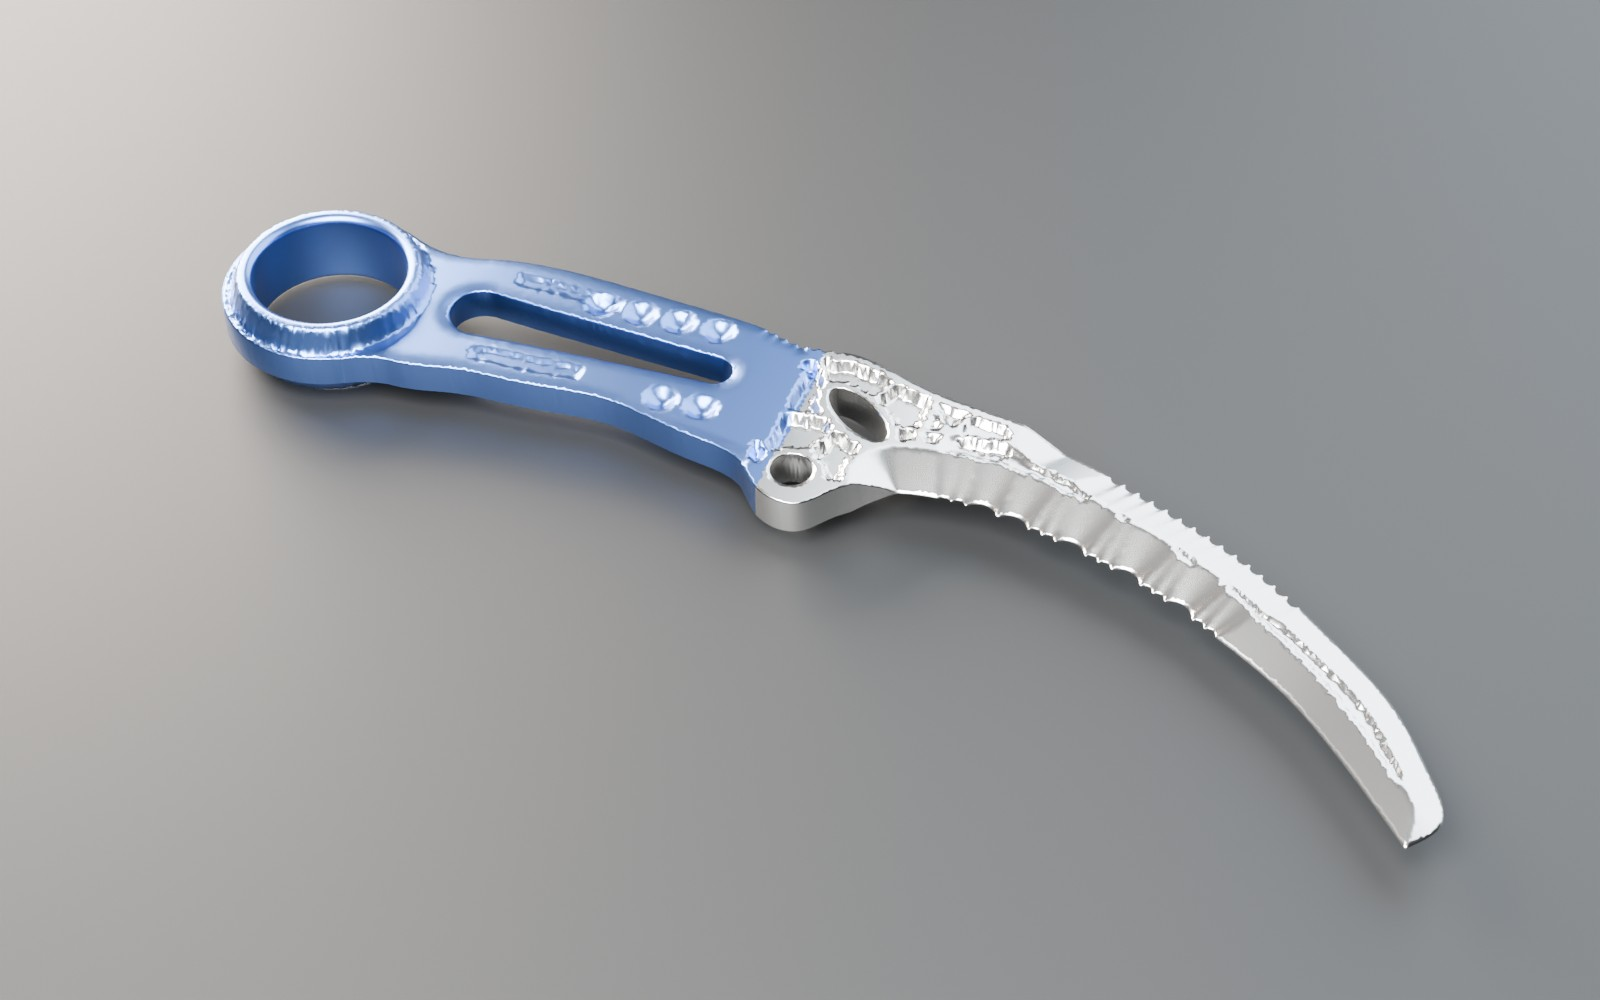
\includegraphics[width=\textwidth]{../../assets/leader/hero.jpg}
\caption{Leader \texttt{ec2i089\_r01\_p10\_c68}, oblique.}\end{figure*}
\begin{figure*}[t]\centering
\begin{minipage}{0.32\textwidth}\centering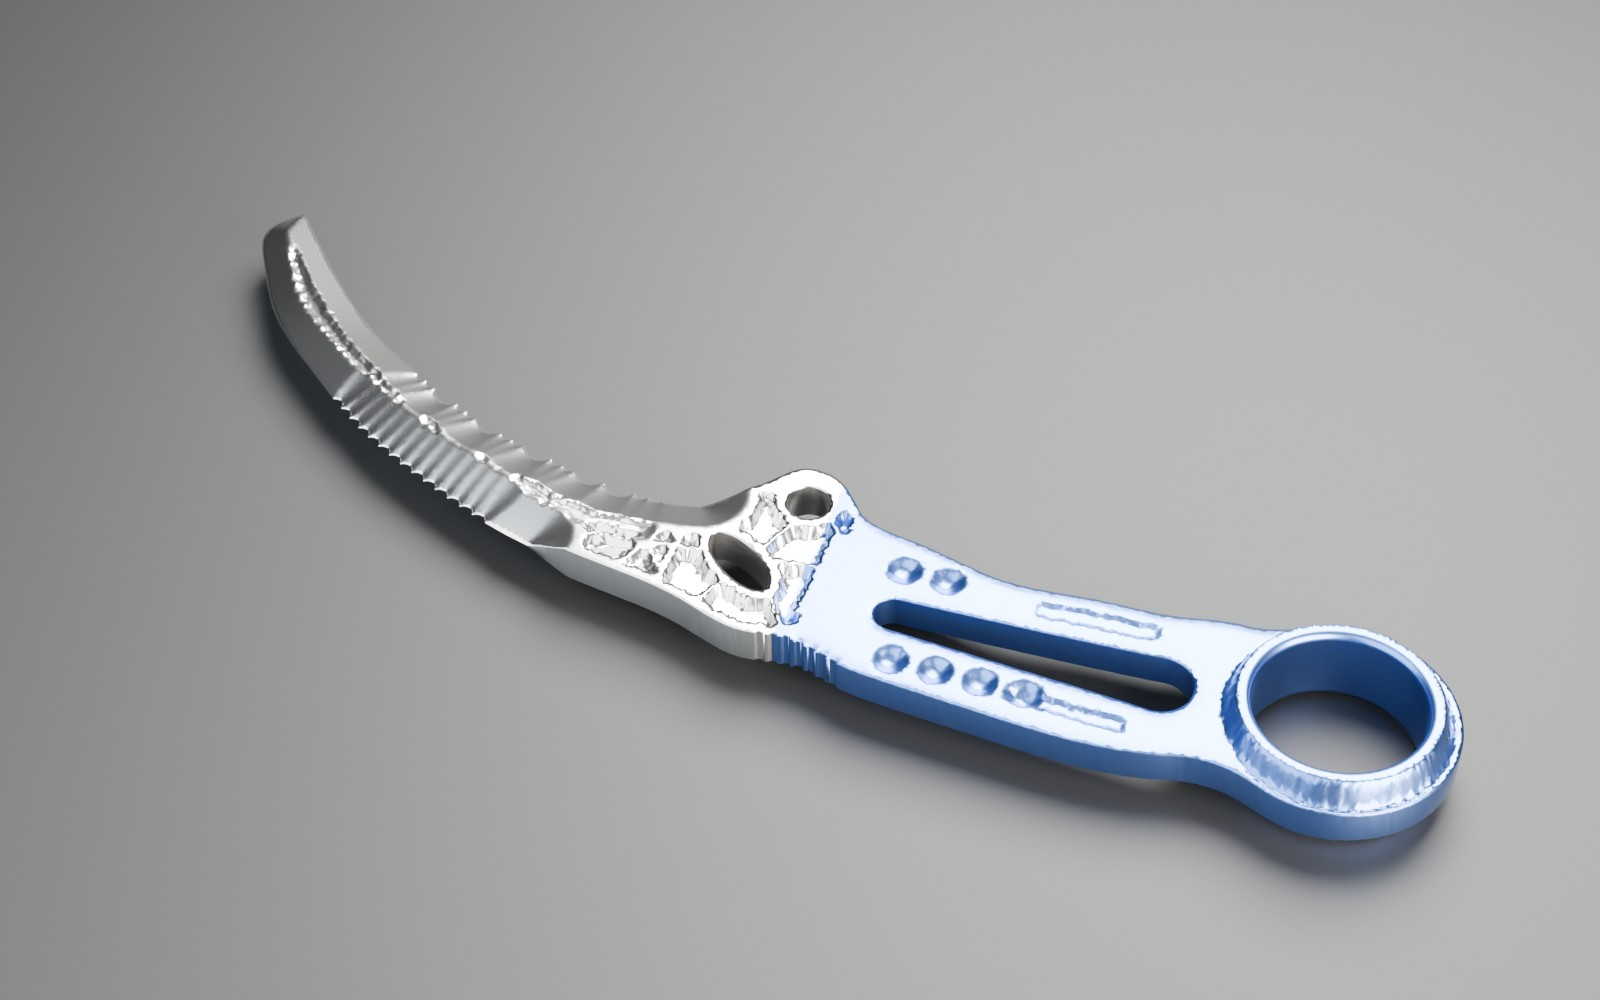
\includegraphics[width=\linewidth]{../../assets/leader/reverse.jpg}\\{\footnotesize Reverse oblique}\end{minipage}\hfill
\begin{minipage}{0.32\textwidth}\centering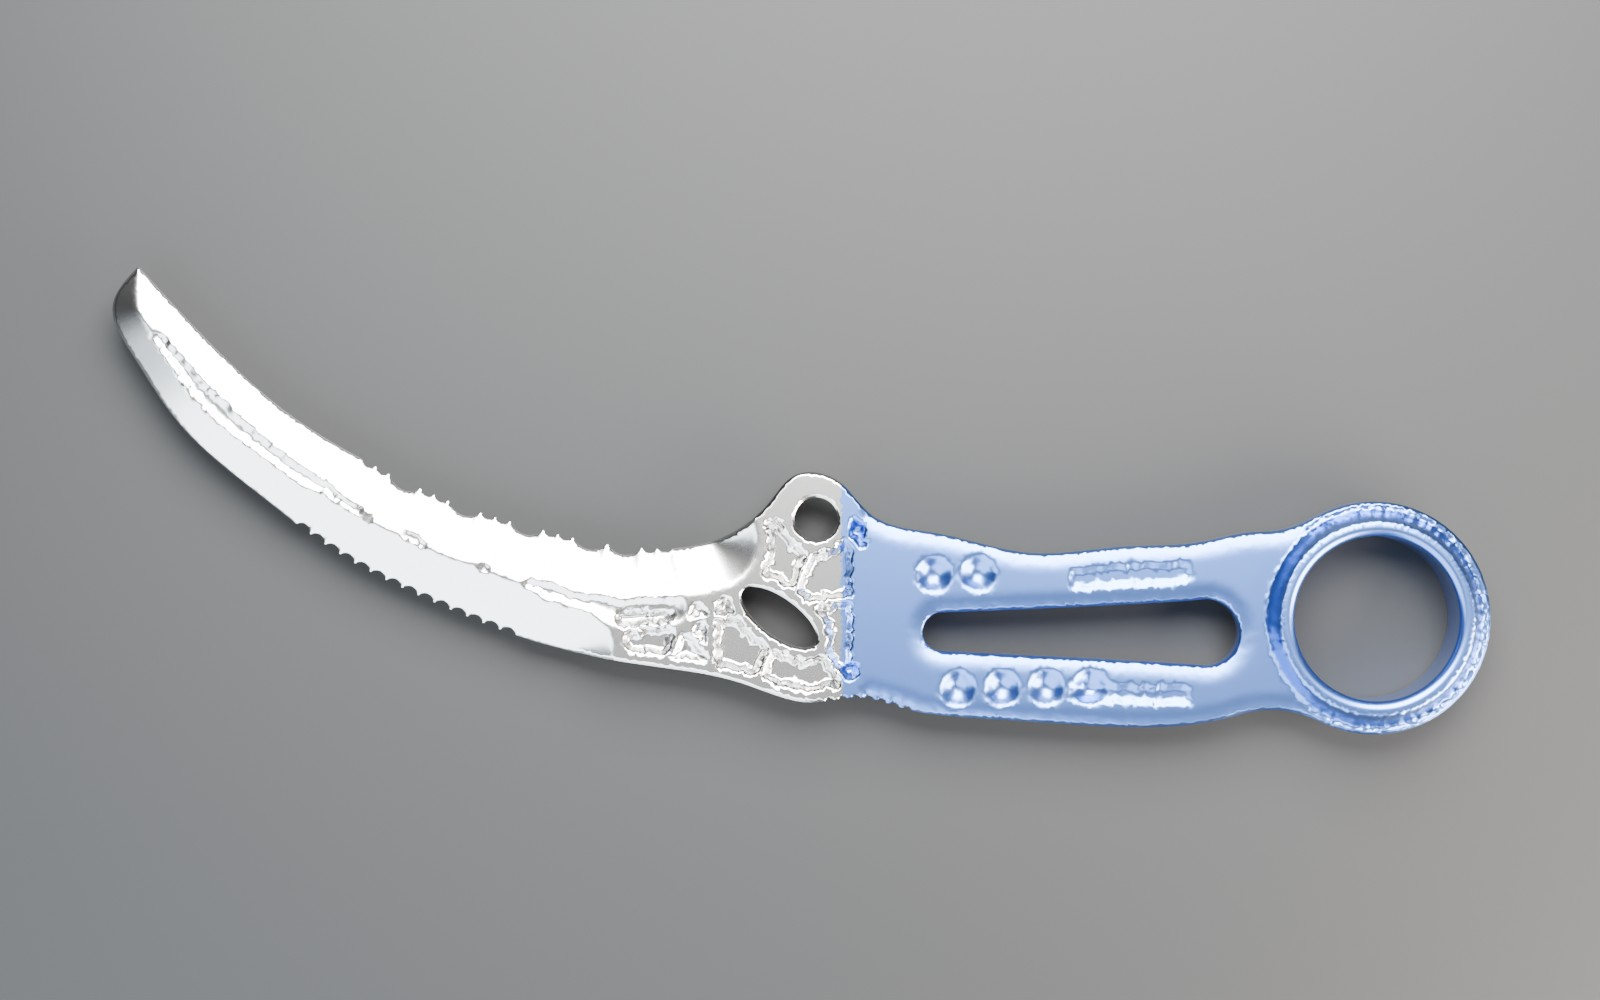
\includegraphics[width=\linewidth]{../../assets/leader/side.jpg}\\{\footnotesize Plan view}\end{minipage}\hfill
\begin{minipage}{0.32\textwidth}\centering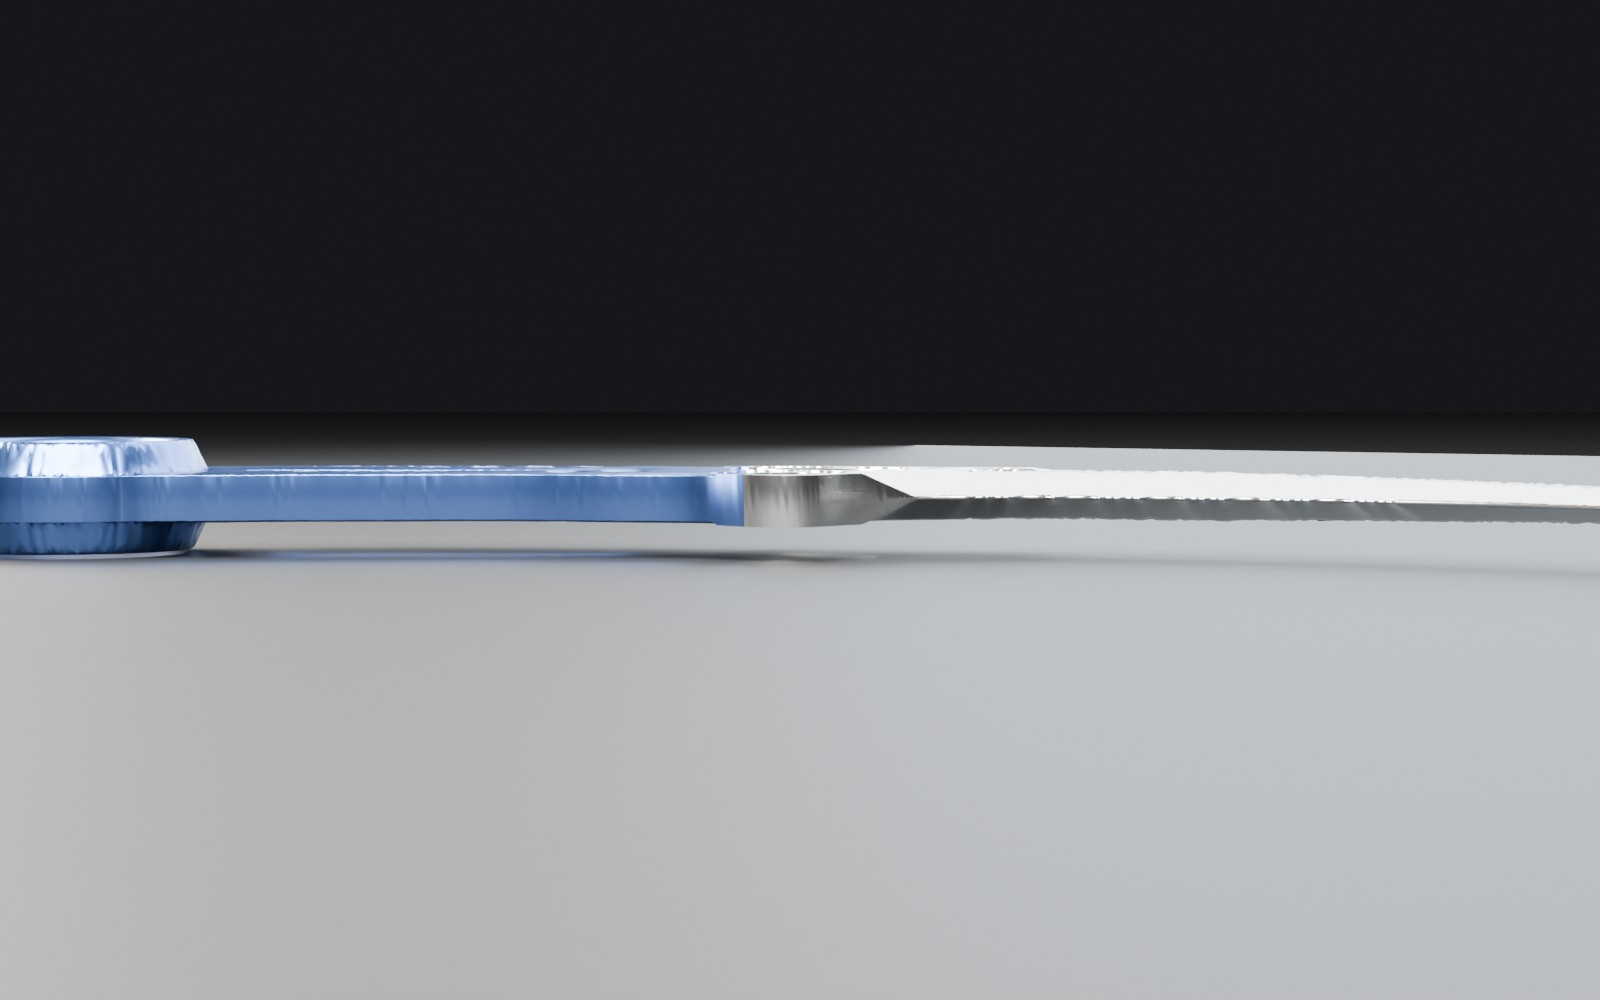
\includegraphics[width=\linewidth]{../../assets/leader/top.jpg}\\{\footnotesize Edge-on}\end{minipage}\\[4pt]
\begin{minipage}{0.32\textwidth}\centering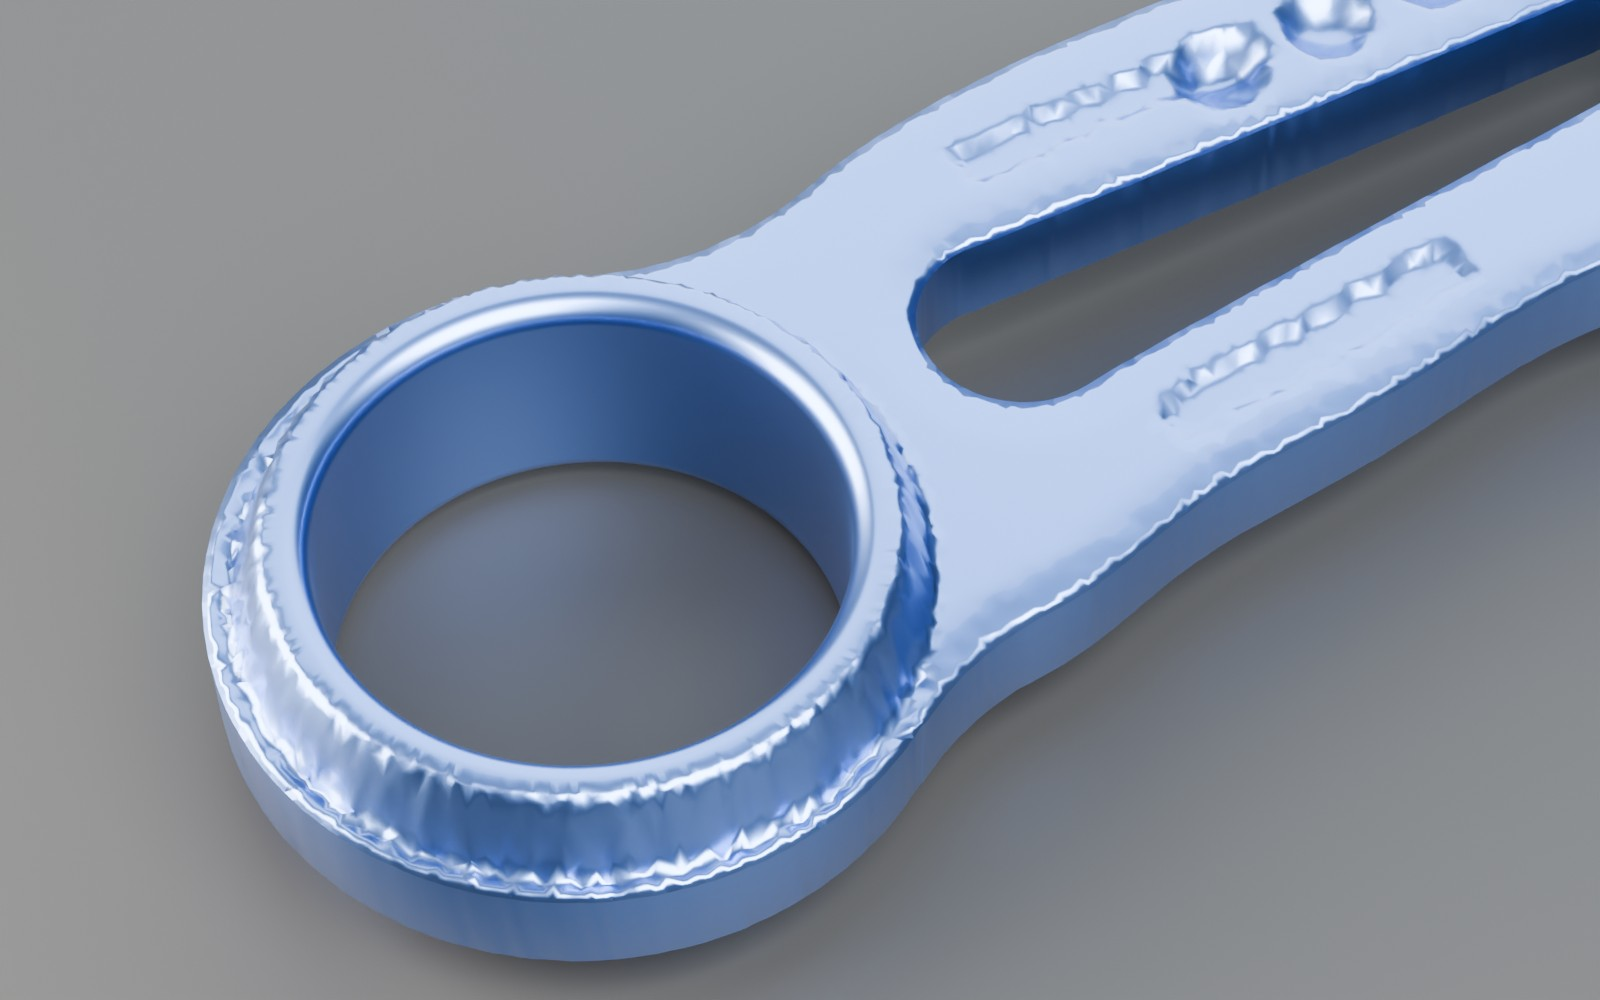
\includegraphics[width=\linewidth]{../../assets/leader/ring.jpg}\\{\footnotesize Ring}\end{minipage}\hfill
\begin{minipage}{0.32\textwidth}\centering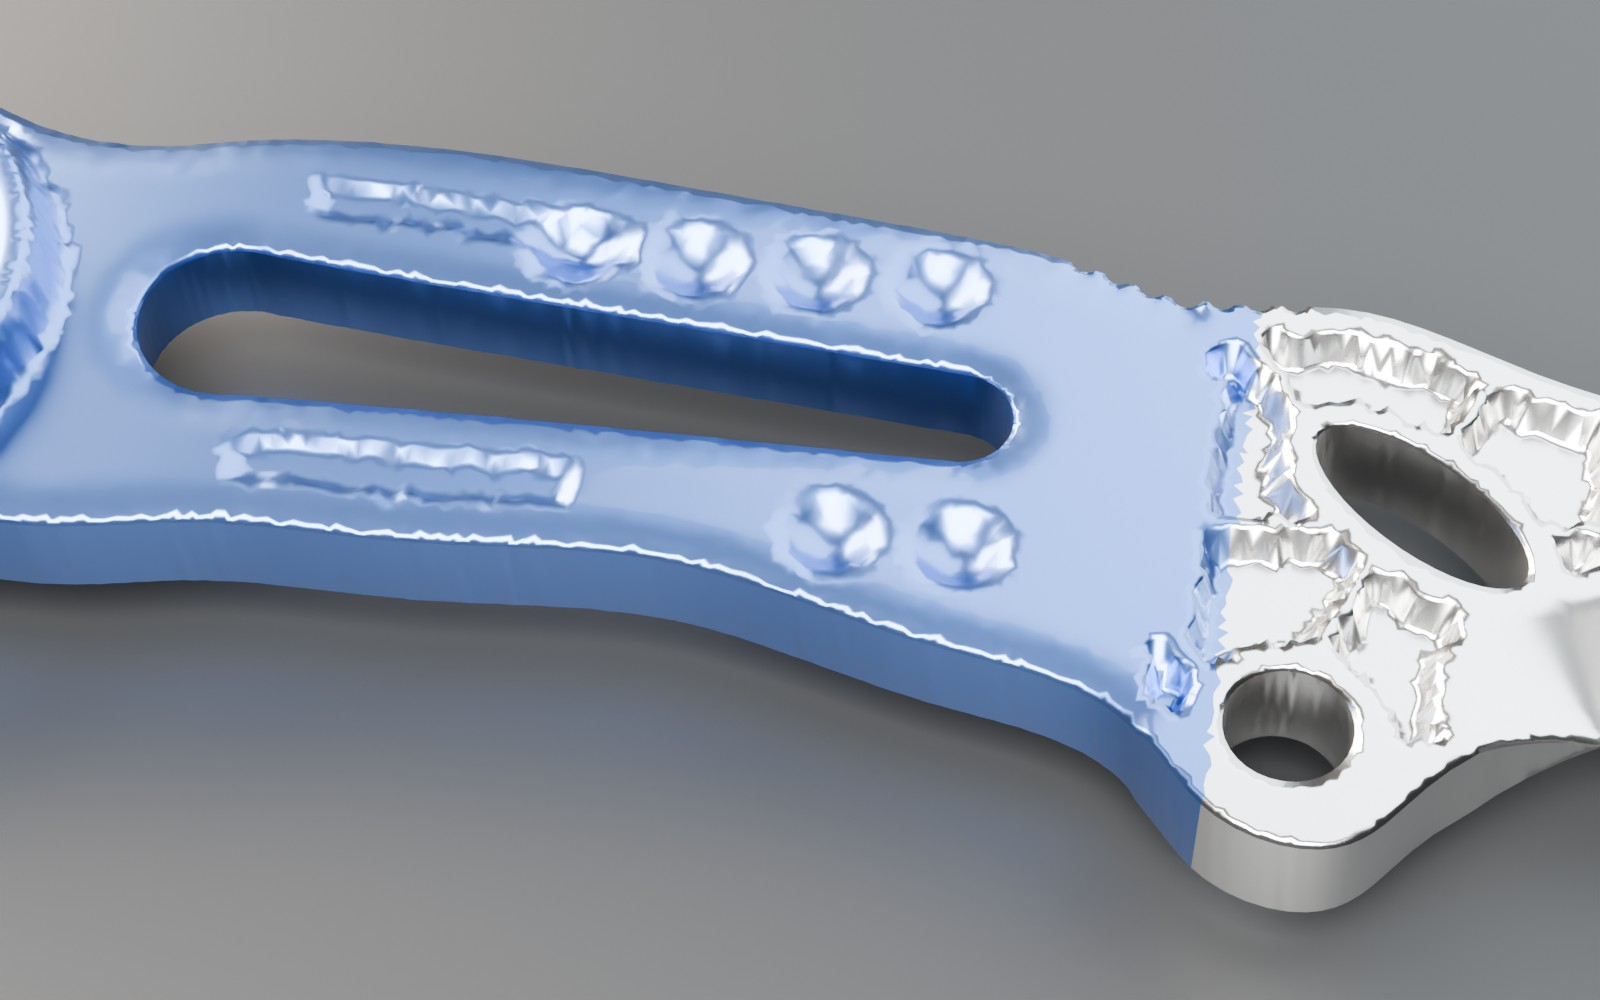
\includegraphics[width=\linewidth]{../../assets/leader/grip.jpg}\\{\footnotesize Grip and pockets}\end{minipage}\hfill
\begin{minipage}{0.32\textwidth}\centering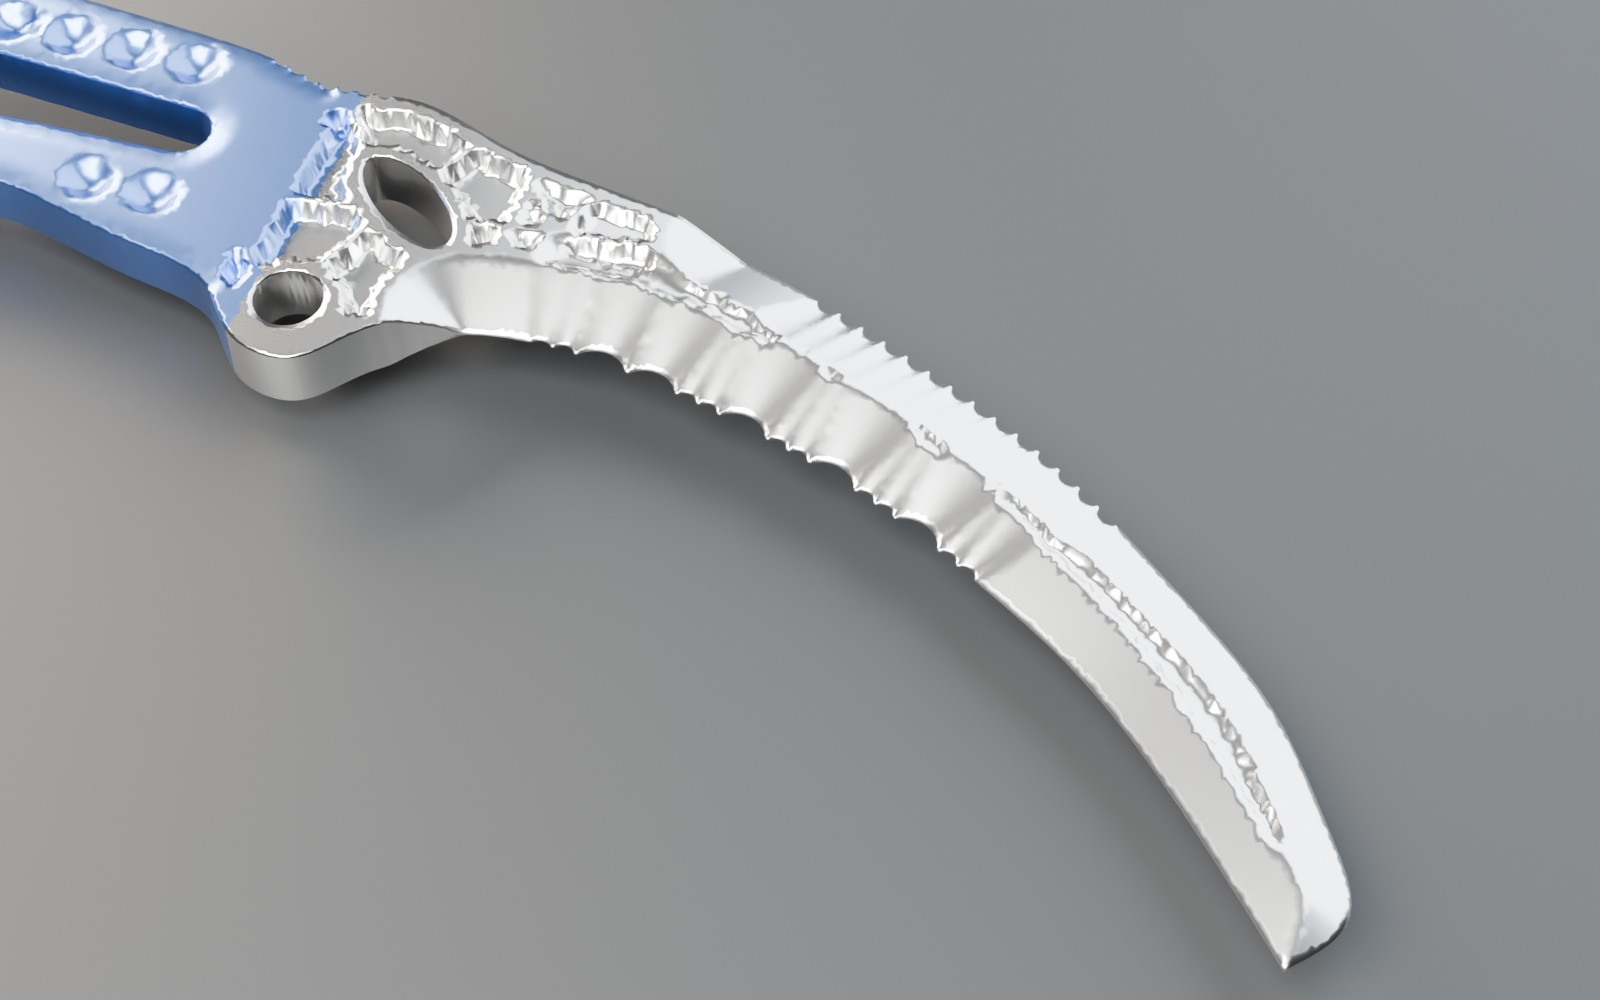
\includegraphics[width=\linewidth]{../../assets/leader/blade.jpg}\\{\footnotesize Blade}\end{minipage}\\[4pt]
\begin{minipage}{0.32\textwidth}\centering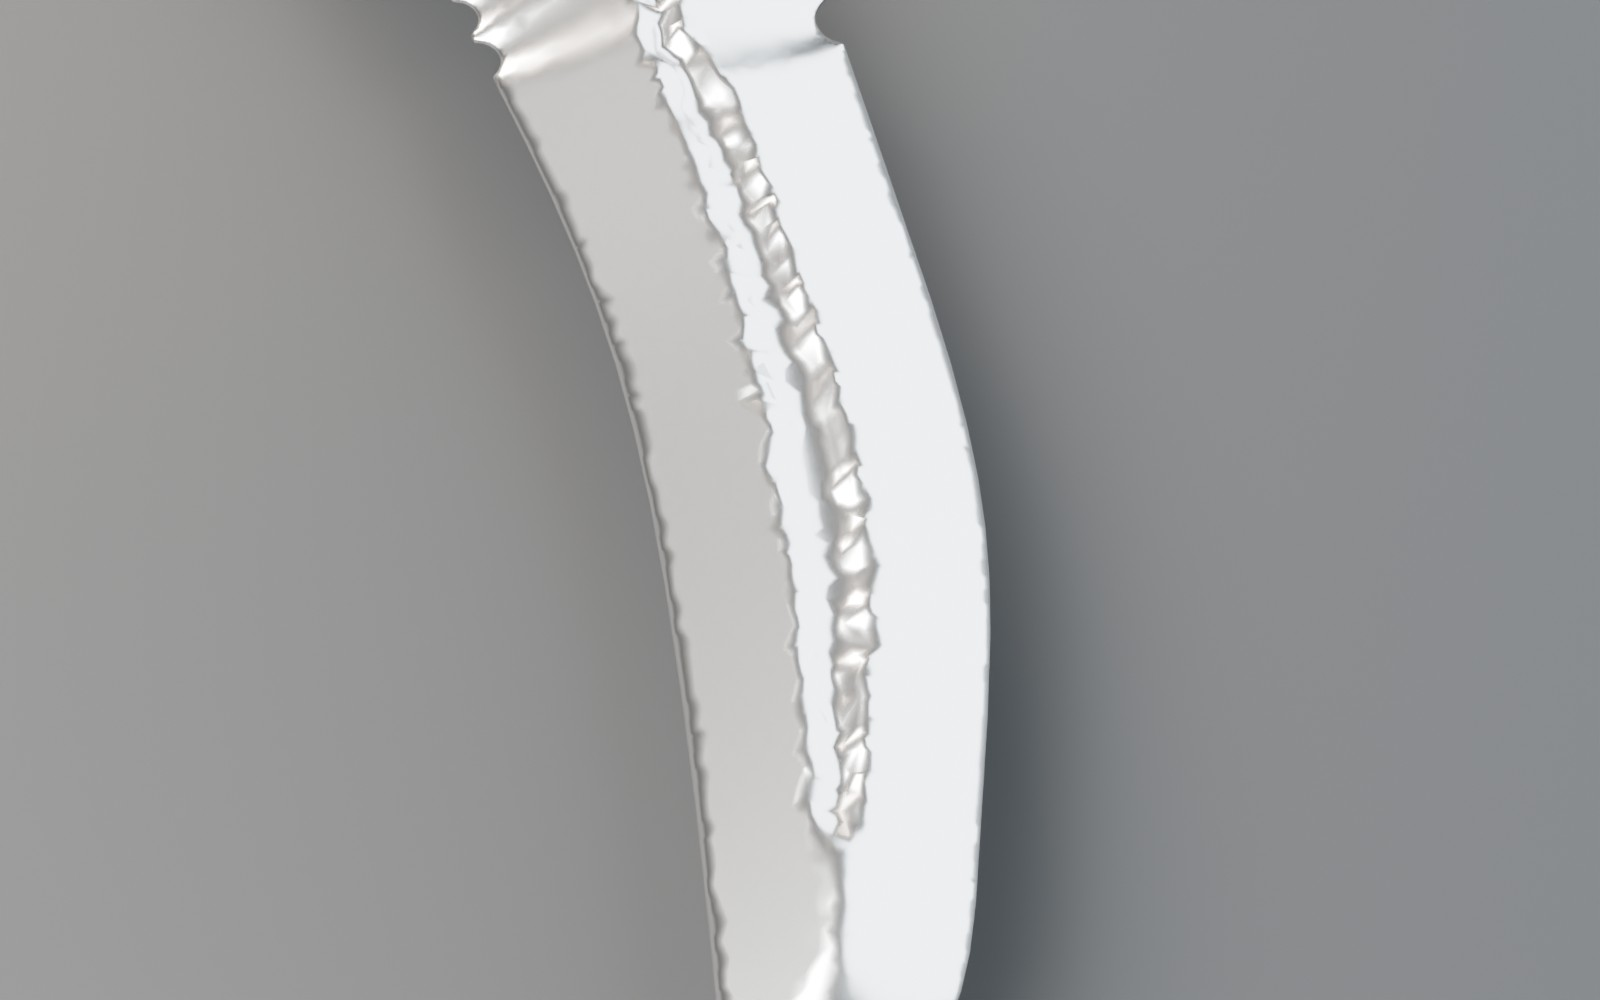
\includegraphics[width=\linewidth]{../../assets/leader/tip.jpg}\\{\footnotesize The point}\end{minipage}\hfill
\begin{minipage}{0.32\textwidth}\centering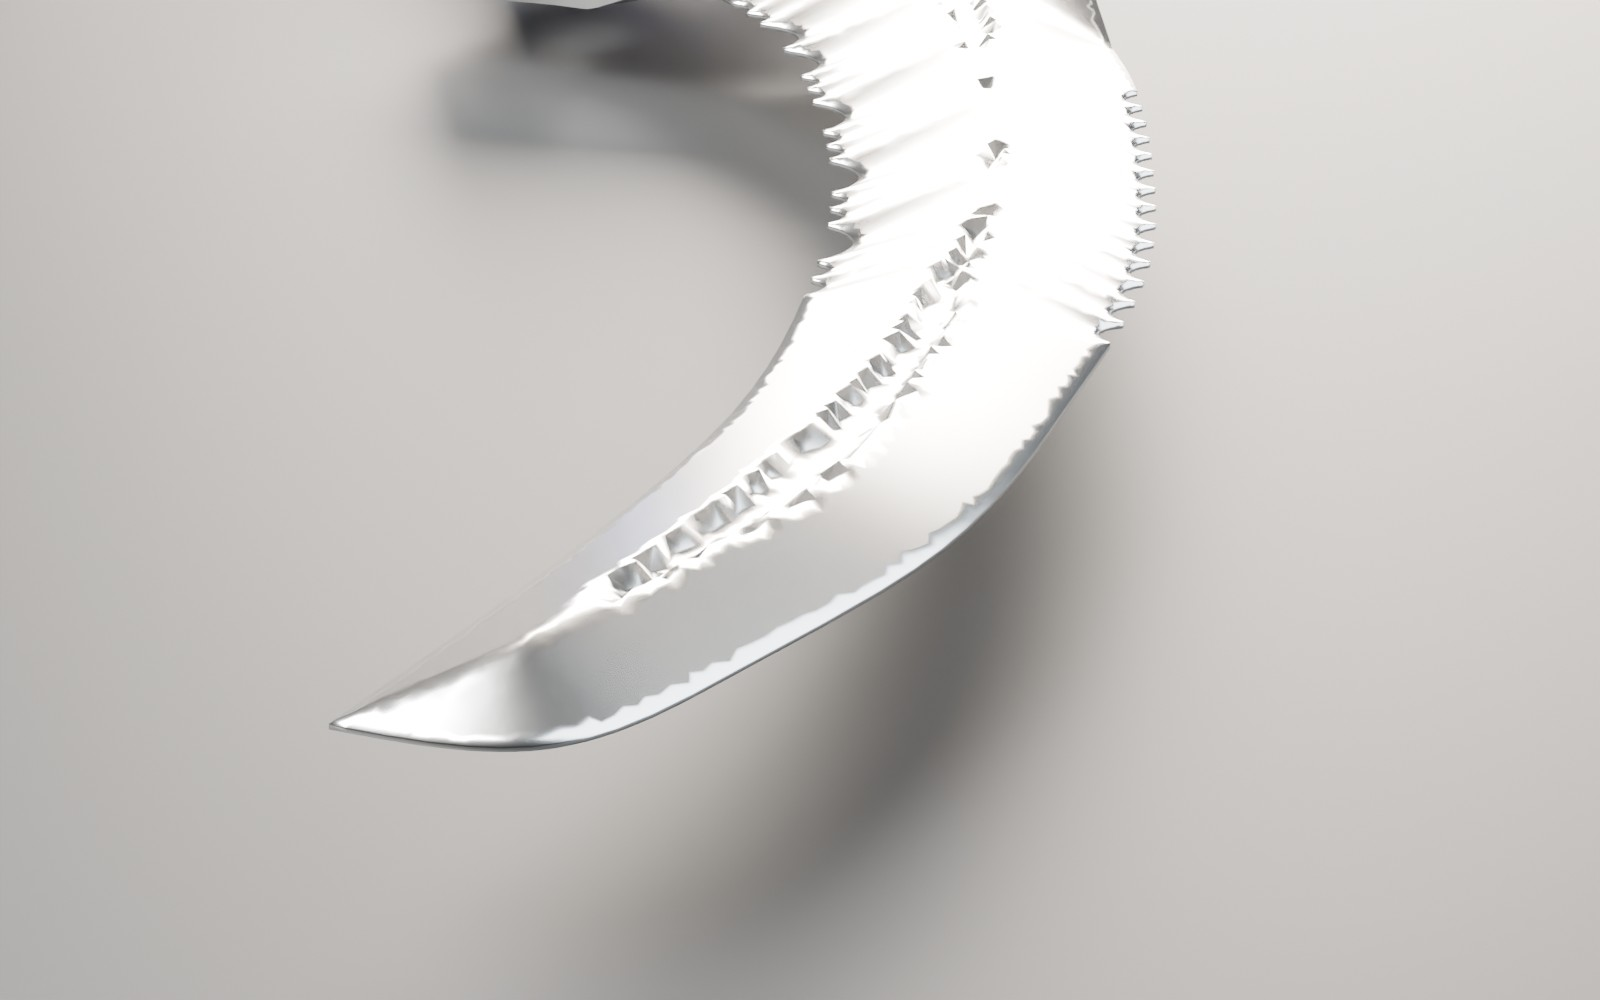
\includegraphics[width=\linewidth]{../../assets/leader/tip_edge.jpg}\\{\footnotesize Edge at the point}\end{minipage}\hfill
\begin{minipage}{0.32\textwidth}\centering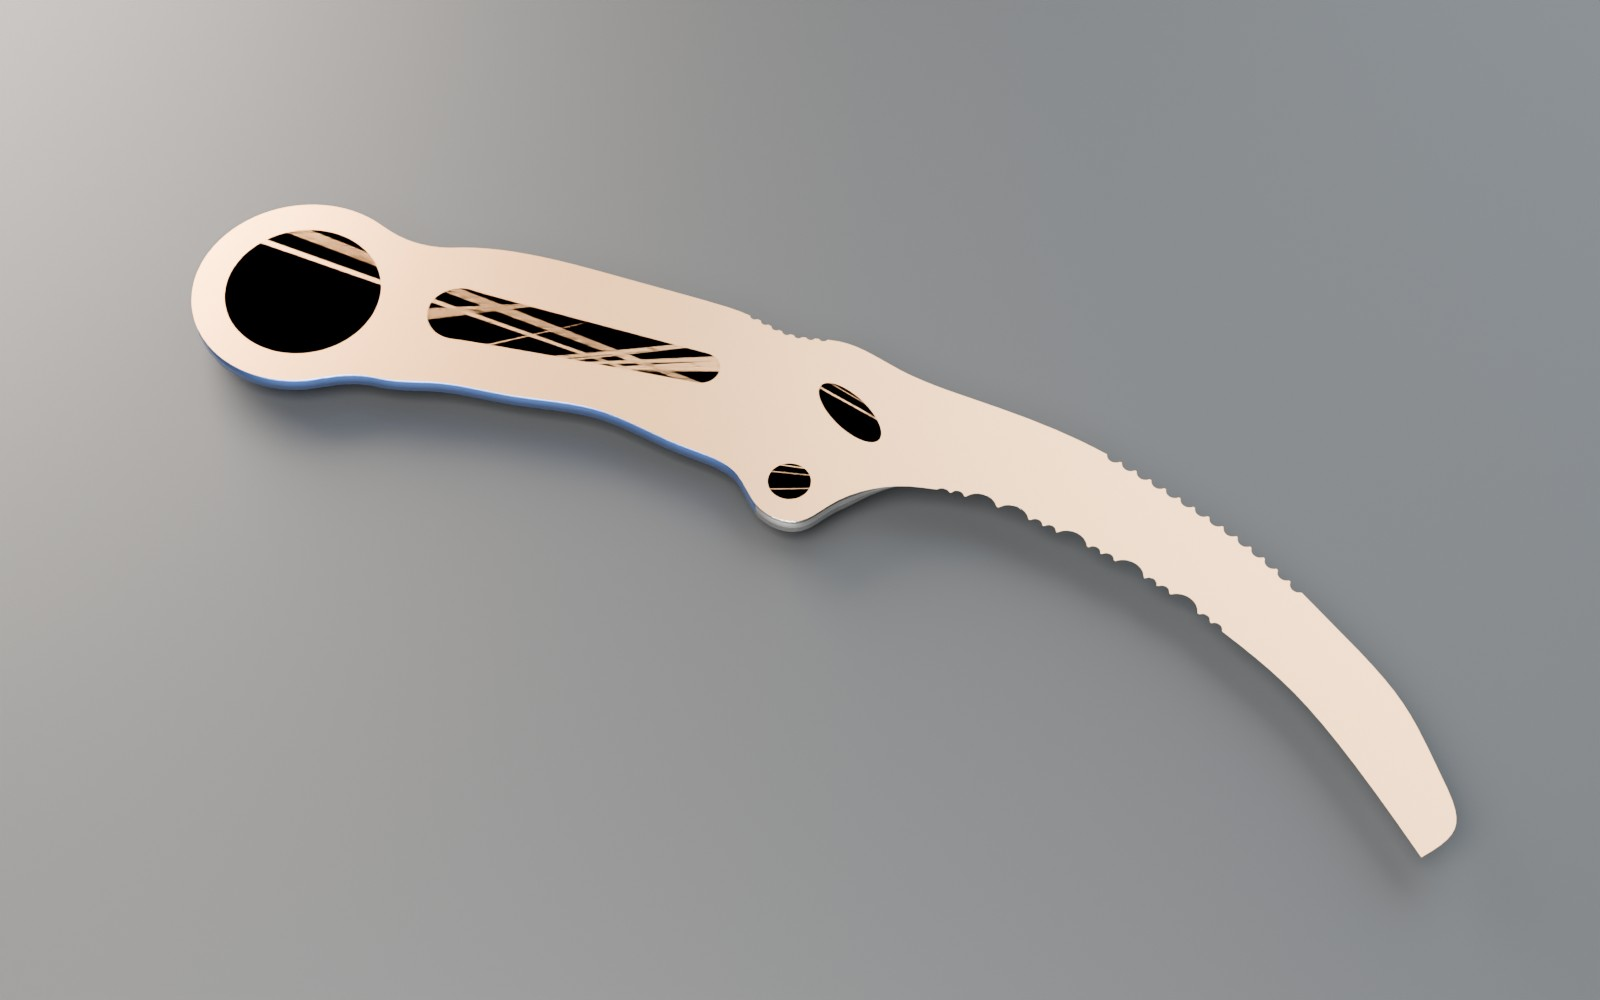
\includegraphics[width=\linewidth]{../../assets/leader/cut_full.jpg}\\{\footnotesize Mid-plane cut (z = 0)}\end{minipage}\\[4pt]
\begin{minipage}{0.32\textwidth}\centering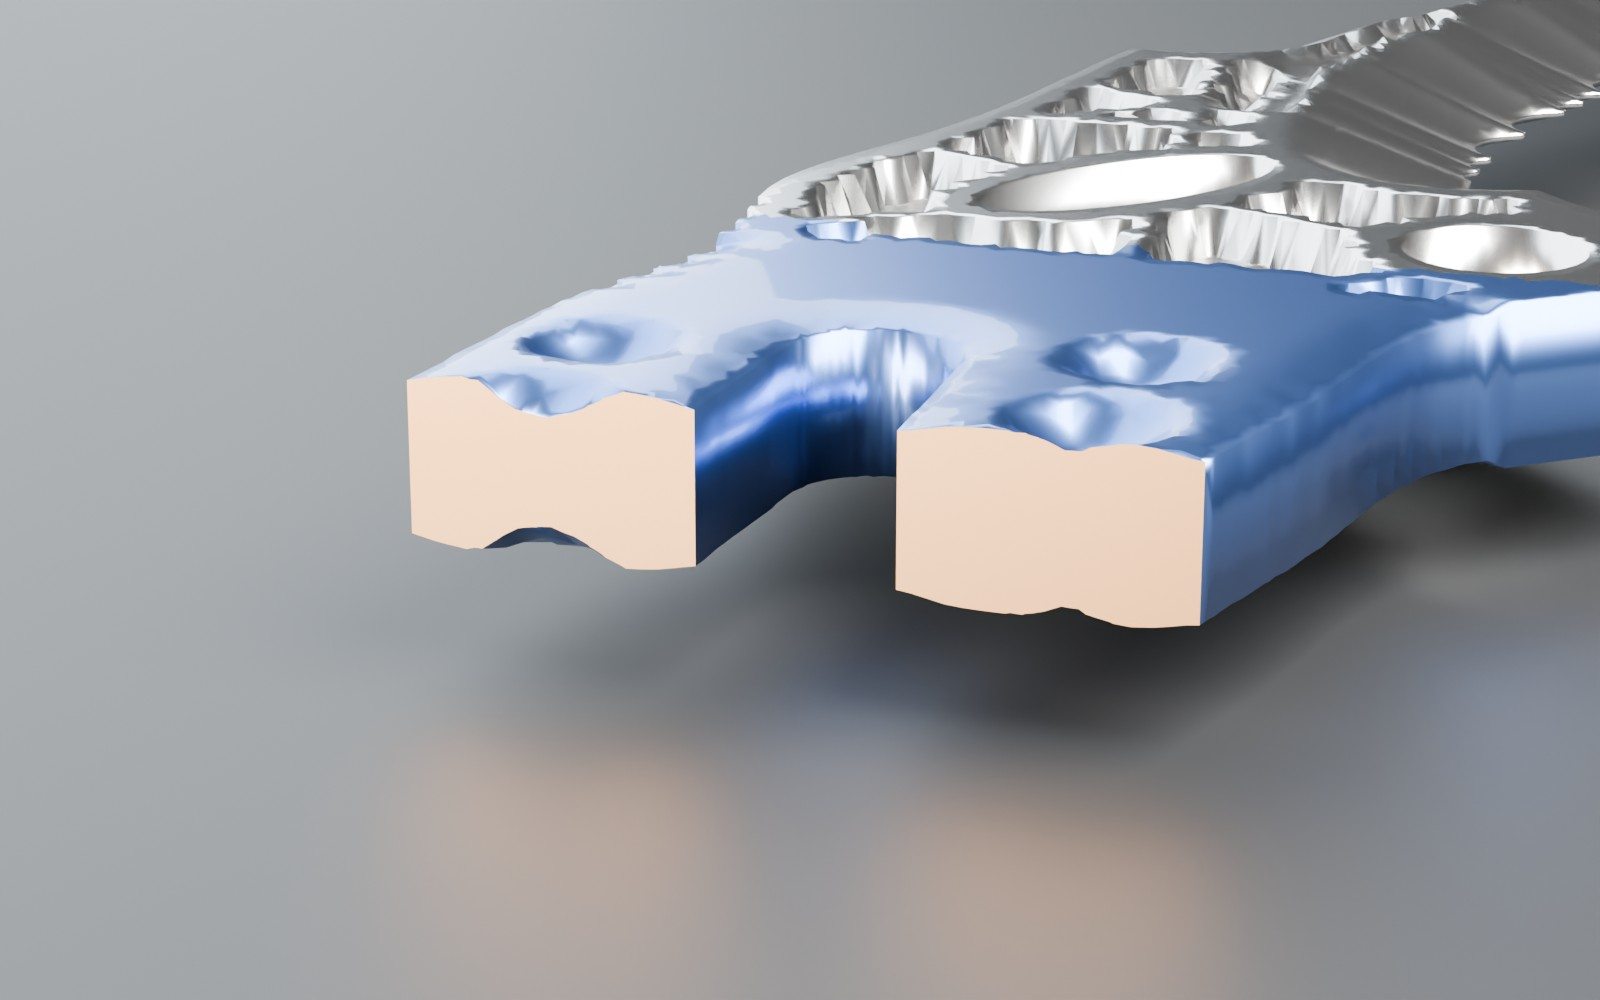
\includegraphics[width=\linewidth]{../../assets/leader/cut_x.jpg}\\{\footnotesize Section across the grip}\end{minipage}\hfill
\begin{minipage}{0.32\textwidth}\centering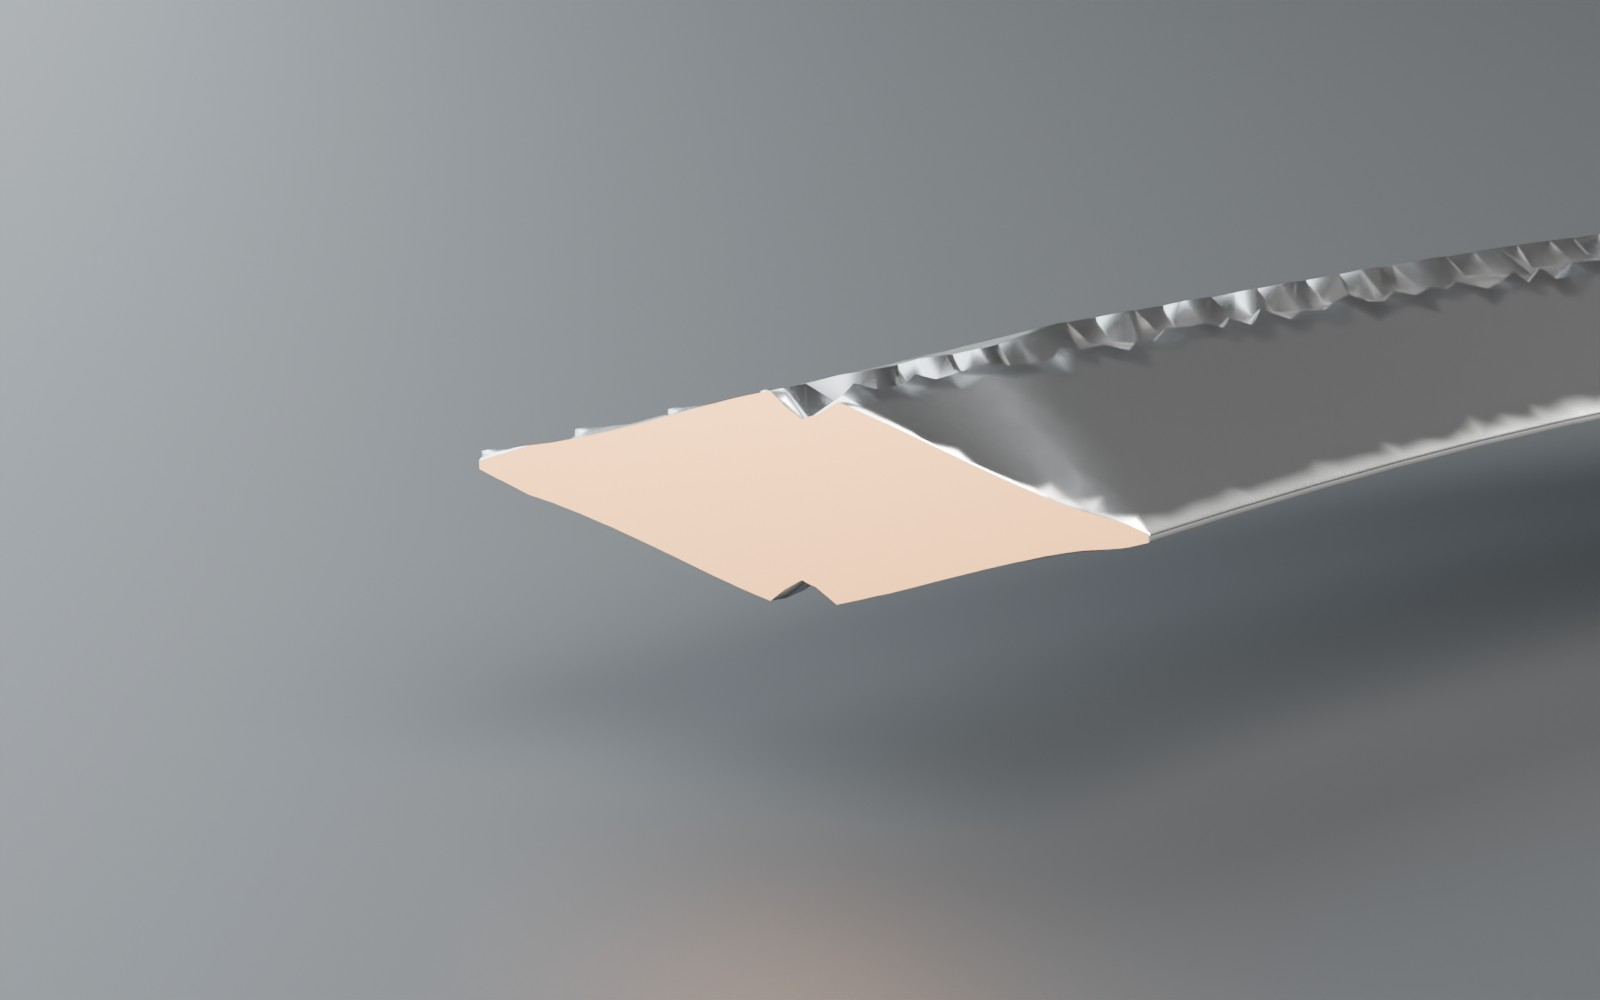
\includegraphics[width=\linewidth]{../../assets/leader/cut_b.jpg}\\{\footnotesize Section across the blade}\end{minipage}\hfill
\caption{All Blender views of the latest-run leader.}\end{figure*}
}{}
\section{Conclusion}\label{sec:conclusion}
Rebuilding the Jarambit pipeline around the literature-sourced requirement set \code{RS-karambit-v5} and the \code{G5.0}
decoder resolved the representation, load-case, drainage, and objective flaws exposed by the G3 diagnostics. Expressing the
grip perimeter, palm-swell aspect ratio, planform point wedge, rounded-gullet serrations, sheet-TPMS wall thickness, and
rib-clear drainage ports directly in requirement units ensured that candidates in the search space have a sharp planform
point, a full-sized ergonomic handle, and width-checked internal drainage. Coupling the 16-case multi-fidelity structural chain
with the multiplicative worst-margin factor $W$ and fifth-power ergonomic multiplier $E^5$ in \code{W\_ERGOLIGHT\_v2}
prevented the search from trading structural adequacy or hand comfort for grams. Across \gEvalsTotal{} evaluations on
\gIslands{} islands, evolutionary search outperformed the equal-budget scrambled-Sobol baseline (\gScore{} vs.\
\gBaselineBest) and produced the best individual \gDesign{} at \gMassFinishedG{}~g finished partial-volume mass (\gMassG{}~g
print mesh) with worst structural margin ratio $\mu = \gWorstMarginRatio$ ($W = \gW$, every load case met) and ergonomic
multiplier $E = \gE$. Physical L-PBF printing, stress relief, CNC bevel grinding, and mechanical testing under the ten open
evidence gaps in Section~\ref{sec:limits} remain the necessary next step before any operational qualification.


\begin{thebibliography}{75}
\bibitem{mouret2015} J.-B. Mouret and J. Clune, ``Illuminating search spaces by mapping elites,'' \emph{arXiv:1504.04909}, 2015.
\bibitem{vassiliades2018} V. Vassiliades, K. Chatzilygeroudis, and J.-B. Mouret, ``Using centroidal Voronoi tessellations to scale up the multidimensional archive of phenotypic elites algorithm,'' \emph{IEEE Trans. Evol. Comput.}, vol. 22, no. 4, pp. 623--630, 2018.
\bibitem{vassiliades2018b} V. Vassiliades and J.-B. Mouret, ``Discovering the elite hypervolume by leveraging interspecies correlation,'' in \emph{Proc. GECCO}, 2018.
\bibitem{lloyd1982} S. P. Lloyd, ``Least squares quantization in PCM,'' \emph{IEEE Trans. Inf. Theory}, vol. 28, no. 2, pp. 129--137, 1982, doi:10.1109/TIT.1982.1056489.
\bibitem{joe2008} S. Joe and F. Y. Kuo, ``Constructing Sobol sequences with better two-dimensional projections,'' \emph{SIAM J. Sci. Comput.}, vol. 30, no. 5, pp. 2635--2654, 2008.
\bibitem{matousek1998} J. Matou\v{s}ek, ``On the $L_2$-discrepancy for anchored boxes,'' \emph{J. Complexity}, vol. 14, no. 4, pp. 527--556, 1998.
\bibitem{doi1991} A. Doi and A. Koide, ``An efficient method of triangulating equi-valued surfaces by using tetrahedral cells,'' \emph{IEICE Trans. Inf. Syst.}, vol. E74-D, no. 1, pp. 214--224, 1991.
\bibitem{lorensen1987} W. E. Lorensen and H. E. Cline, ``Marching cubes: A high resolution 3D surface construction algorithm,'' \emph{Comput. Graph.}, vol. 21, no. 4, pp. 163--169, 1987.
\bibitem{batoz1980} J.-L. Batoz, K.-J. Bathe, and L.-W. Ho, ``A study of three-node triangular plate bending elements,'' \emph{Int. J. Numer. Methods Eng.}, vol. 15, no. 12, pp. 1771--1812, 1980, doi:10.1002/nme.1620151205.
\bibitem{roache1998} P. J. Roache, \emph{Verification and Validation in Computational Science and Engineering}. Albuquerque, NM: Hermosa Publishers, 1998.
\bibitem{inglis1913} C. E. Inglis, ``Stresses in a plate due to the presence of cracks and sharp corners,'' \emph{Trans. Inst. Naval Archit.}, vol. 55, pp. 219--241, 1913.
\bibitem{timoshenko1961} S. P. Timoshenko and J. M. Gere, \emph{Theory of Elastic Stability}, 2nd ed. New York: McGraw-Hill, 1961.
\bibitem{f2924} ASTM F2924-14(2021), \emph{Standard Specification for Additive Manufacturing Titanium-6 Aluminum-4 Vanadium with Powder Bed Fusion}, ASTM International, 2021.
\bibitem{hdbk5j} U.S. Department of Defense, \emph{MIL-HDBK-5J: Metallic Materials and Elements for Aerospace Vehicle Structures}, \S 5.4.1 (Ti-6Al-4V annealed: Table 5.4.1.0(b); Figs.~5.4.1.1.1 and 5.4.1.1.4), 2003.
\bibitem{ncamp} NIAR/NCAMP, \emph{ND-ME 004: L-PBF Ti-6Al-4V Material Specification}, 2025.
\bibitem{nasa6030} NASA, \emph{NASA-STD-6030: Additive Manufacturing Requirements for Spaceflight Systems}, 2021.
\bibitem{eos} EOS GmbH, \emph{EOS Titanium Ti64 Grade 5 Material Data Sheet (M290)}.
\bibitem{vrancken2012} B. Vrancken, L. Thijs, J.-P. Kruth, and J. Van Humbeeck, ``Heat treatment of Ti6Al4V produced by selective laser melting,'' \emph{J. Alloys Compd.}, vol. 541, p. 177, 2012, doi:10.1016/j.jallcom.2012.07.022.
\bibitem{cain2015} V. Cain \emph{et al.}, ``Crack propagation and fracture toughness of Ti6Al4V alloy produced by selective laser melting,'' \emph{Addit. Manuf.}, vol. 5, p. 68, 2015, doi:10.1016/j.addma.2014.12.006.
\bibitem{xie2026} Y. Xie \emph{et al.}, \emph{Materials}, vol. 19, art. 1945, 2026, doi:10.3390/ma19101945.
\bibitem{murchio2024} S. Murchio \emph{et al.}, \emph{Int. J. Fatigue}, vol. 180, art. 108102, 2024, doi:10.1016/j.ijfatigue.2023.108102.
\bibitem{benedetti2018} M. Benedetti \emph{et al.}, \emph{Int. J. Fatigue}, vol. 107, p. 96, 2018, doi:10.1016/j.ijfatigue.2017.10.021.
\bibitem{nicoletto2018} G. Nicoletto, \emph{Int. J. Fatigue}, vol. 106, p. 124, 2018, doi:10.1016/j.ijfatigue.2017.10.004.
\bibitem{wycisk2014} E. Wycisk \emph{et al.}, \emph{Phys. Procedia}, vol. 56, p. 371, 2014, doi:10.1016/j.phpro.2014.08.120.
\bibitem{wycisk2015} E. Wycisk \emph{et al.}, \emph{Front. Mater.}, vol. 2, art. 72, 2015, doi:10.3389/fmats.2015.00072.
\bibitem{pagliari2025} L. Pagliari \emph{et al.}, \emph{Eng. Fail. Anal.}, vol. 180, art. 109825, 2025, doi:10.1016/j.engfailanal.2025.109825.
\bibitem{johnsen2024} J. Johnsen \emph{et al.}, \emph{Welding in the World}, vol. 68, p. 361, 2024, doi:10.1007/s40194-023-01604-5.
\bibitem{kahlin2017} M. Kahlin, H. Ansell, and J. Moverare, \emph{Int. J. Fatigue}, vol. 101, p. 51, 2017, doi:10.1016/j.ijfatigue.2017.04.009.
\bibitem{beretta2017} S. Beretta and S. Romano, \emph{Int. J. Fatigue}, vol. 94, p. 178, 2017, doi:10.1016/j.ijfatigue.2016.06.020.
\bibitem{barricelli2022} L. Barricelli, L. Patriarca, A. du Plessis, and S. Beretta, \emph{Int. J. Fatigue}, art. 107401, 2022, doi:10.1016/j.ijfatigue.2022.107401.
\bibitem{naghavi2022} S. A. Naghavi \emph{et al.}, \emph{Bioengineering}, vol. 9, art. 504, 2022, doi:10.3390/bioengineering9100504.
\bibitem{timercan2021} A. Timercan, V. Sheremetyev, and V. Brailovski, \emph{Sci. Technol. Adv. Mater.}, vol. 22, p. 285, 2021, doi:10.1080/14686996.2021.1907222.
\bibitem{kelly2019} C. N. Kelly \emph{et al.}, \emph{Acta Biomater.}, vol. 94, p. 610, 2019, doi:10.1016/j.actbio.2019.05.046.
\bibitem{lietaert2018} K. Lietaert \emph{et al.}, \emph{Sci. Rep.}, vol. 8, art. 4957, 2018, doi:10.1038/s41598-018-23414-2.
\bibitem{benedetti2021} M. Benedetti, A. du Plessis \emph{et al.}, \emph{Mater. Sci. Eng. R}, vol. 144, art. 100606, 2021, doi:10.1016/j.mser.2021.100606.
\bibitem{alana2021} M. Ala\~{n}a \emph{et al.}, \emph{Sci. Rep.}, vol. 11, 2021, doi:10.1038/s41598-021-98631-3.
\bibitem{renishaw2017} Renishaw, \emph{Design for Metal AM: A Beginner's Guide}, 2017.
\bibitem{carrozza2023} A. Carrozza, B. Bircher, A. Aversa, and S. Biamino, ``Investigating complex geometrical features in LPBF-produced parts: a material-based comparison between different titanium alloys,'' \emph{Met. Mater. Int.}, 2023, doi:10.1007/s12540-023-01460-4.
\bibitem{solukon} Xometry DMLS design guide; Materialise metal design guide; Solukon depowdering guidance (powder ports 2--5~mm, $\ge 3$~mm).
\bibitem{dodds2014} R. M. Dodds \emph{et al.}, ``Grip strength across the life course,'' \emph{PLoS ONE}, vol. 9, art. e113637, 2014, doi:10.1371/journal.pone.0113637.
\bibitem{hidh} NASA, \emph{Human Integration Design Handbook (HIDH)}, NASA/SP-2010-3407/REV1, \S 9.12.2 and App.~B Table~8, 2014.
\bibitem{mil1472h} U.S. Department of Defense, \emph{MIL-STD-1472H: Human Engineering}, \S 5.7.6.3--4 and Fig.~23, 2020.
\bibitem{niosh2004} Cal/OSHA--NIOSH, \emph{Easy Ergonomics: A Guide to Selecting Non-Powered Hand Tools}, Pub. 2004-164, 2004.
\bibitem{kong2005} Y.-K. Kong and B. D. Lowe, ``Optimal cylindrical handle diameter for grip force tasks,'' \emph{Int. J. Ind. Ergon.}, vol. 35, p. 495, 2005, doi:10.1016/j.ergon.2004.11.003.
\bibitem{seo2008hf} N. J. Seo and T. J. Armstrong, ``Investigation of grip force, normal force, contact area, hand size, and handle size for cylindrical handles,'' \emph{Human Factors}, vol. 50, no. 5, pp. 734--744, 2008, doi:10.1518/001872008X354192.
\bibitem{seo2011} N. J. Seo and T. J. Armstrong, ``Effect of elliptic handle shape on \ldots{} twisting ability,'' \emph{Ergonomics}, vol. 54, p. 961, 2011, doi:10.1080/00140139.2011.606923.
\bibitem{ansur2} C. C. Gordon \emph{et al.}, \emph{ANSUR II}, NATICK/TR-15/007, 2014.
\bibitem{faa-hfds} Federal Aviation Administration, \emph{Human Factors Design Standard (HFDS)}, App.~B (Anthropometry).
\bibitem{tirloni2021} S. F. Tirloni \emph{et al.}, ``Cutting force measurement \ldots: a systematic review,'' \emph{EXCLI J.}, vol. 20, p. 727, 2021, doi:10.17179/excli2021-3167.
\bibitem{cochran1986} D. J. Cochran and M. W. Riley, ``An evaluation of knife handle guarding,'' \emph{Human Factors}, vol. 28, p. 295, 1986, doi:10.1177/001872088602800305.
\bibitem{buchholz1988} B. Buchholz, L. J. Frederick, and T. J. Armstrong, \emph{Ergonomics}, vol. 31, p. 317, 1988, doi:10.1080/00140138808966676.
\bibitem{fransson1993} C. Fransson-Hall and \AA. Kilbom, ``Sensitivity of the hand to surface pressure,'' \emph{Appl. Ergon.}, vol. 24, p. 181, 1993.
\bibitem{johansson1999} L. Johansson \emph{et al.}, ``Perception of surface pressure applied to the hand,'' \emph{Ergonomics}, vol. 42, p. 1274, 1999, doi:10.1080/001401399184947.
\bibitem{aldien2005} Y. Aldien \emph{et al.}, \emph{Int. J. Ind. Ergon.}, vol. 35, p. 267, 2005, doi:10.1016/j.ergon.2004.09.005.
\bibitem{osullivan2002} L. W. O'Sullivan and T. J. Gallwey, \emph{J. Electromyogr. Kinesiol.}, vol. 12, p. 275, 2002, doi:10.1016/S1050-6411(02)00014-7.
\bibitem{yoshii2015} Y. Yoshii \emph{et al.}, \emph{BioMed. Eng. OnLine}, vol. 14, art. 115, 2015.
\bibitem{kong2007} Y.-K. Kong \emph{et al.}, \emph{Ergonomics}, 2007 (screwdriving torque).
\bibitem{mcgorry2005} R. W. McGorry, P. C. Dowd, and P. G. Dempsey, \emph{Appl. Ergon.}, 2005 (moments in knife use).
\bibitem{walilko2005} T. J. Walilko, D. C. Viano, and C. A. Bir, ``Biomechanics of the head for Olympic boxer punches to the face,'' \emph{Br. J. Sports Med.}, vol. 39, no. 10, pp. 710--719, 2005.
\bibitem{en8442} EN/ISO 8442-1 and -2, handle twist tests (via CATRA).
\bibitem{iso8442-5} ISO 8442-5:2004, \emph{Materials and Articles in Contact with Foodstuffs---Cutlery and Table Holloware---Part 5: Specification for Sharpness and Edge Retention Test of Cutlery}, 2004.
\bibitem{gost51501} GOST R 51501-99, tourist knives, Clause 9.5.1, 1999.
\bibitem{mil8662e} U.S. Department of Defense, \emph{MIL-K-8662E: Pilot Survival Knife}, 1974.
\bibitem{mil810h} U.S. Department of Defense, \emph{MIL-STD-810H}, Method 516.8, Procedure IV.
\bibitem{fl1} ANSI/PLATO FL1-2019 (drop $\ge 1$~m onto concrete).
\bibitem{en388} EN 388 puncture levels (20 / 60 / 100 / 150~N).
\bibitem{gilchrist2008} M. D. Gilchrist \emph{et al.}, \emph{Forensic Sci. Int.}, vol. 177, p. 52, 2008.
\bibitem{nolan2013} G. Nolan, S. V. Hainsworth, and G. N. Rutty, \emph{J. Forensic Sci.}, vol. 58, p. 372, 2013.
\bibitem{hainsworth2008} S. V. Hainsworth \emph{et al.}, \emph{Int. J. Legal Med.}, vol. 122, p. 281, 2008, doi:10.1007/s00414-007-0202-6.
\bibitem{thomas2018} L. Thomas, \texttt{knifesteelnerds.com}, CATRA regression and edge-geometry articles, 2018.
\bibitem{zhang2023} Y. Zhang \emph{et al.}, \emph{Materials}, vol. 16, art. 5375, 2023.
\bibitem{landes2006} R. Landes, \emph{Messerklingen und Stahl}, 2006 (via Thomas).
\bibitem{us4823467} U.S. Patent 4,823,467 (serrated knife).
\end{thebibliography}
\end{document}
